\documentclass{article}
\usepackage[utf8]{inputenc}
%\usepackage{fullpage}
\usepackage[margin=2.5cm]{geometry}
%Examples
\usepackage{linguex}

%Tables
\usepackage{multirow}
\usepackage[table]{xcolor}
\definecolor{blue}{HTML}{4E60F0}
\usepackage{colortbl}

%Math
\usepackage{amssymb, stmaryrd}
\usepackage[fleqn]{amsmath}

%Graphics
\usepackage{graphicx}
\graphicspath{{./fig/}}
\usepackage{subcaption}
\usepackage{tikz}
\usetikzlibrary{matrix,positioning}

%Comments
%MORA
\newcommand{\changeMM}[2]{{\leavevmode\color{red}{\scriptsize\st{#1}}~\color{red}#2}}
\newcommand{\nbMM}[1]{{\leavevmode\color{red}{\scriptsize#1}}}
\newcommand{\addMM}[1]{{\leavevmode\color{red}#1}}

%EWAN
\newcommand{\changeED}[2]{{\leavevmode\color{blue}{\scriptsize\st{#1}}~\color{blue}#2}}
\newcommand{\nbED}[1]{{\leavevmode\color{blue}{\scriptsize#1}}}
\newcommand{\addED}[1]{{\leavevmode\color{blue}#1}}

%EMMANUEL
\newcommand{\changeEC}[2]{{\leavevmode\color{green}{\scriptsize\st{#1}}~\color{green}#2}}
\newcommand{\nbEC}[1]{{\leavevmode\color{green}{\scriptsize#1}}}
\newcommand{\addEC}[1]{{\leavevmode\color{green}#1}}


%References and bibliography
\usepackage{hyperref}
\usepackage[noabbrev,capitalise,nameinlink]{cleveref}
\hypersetup{colorlinks={true},linkcolor={blue},citecolor=magenta}
\usepackage{natbib}
\bibliographystyle{abbrvnat}

%Line numbers
\usepackage{lineno}
\linenumbers




\title{Mouse tracking as a window into decision making}
\author{Mora Maldonado, Ewan Dunbar \& Emmanuel Chemla}

\begin{document}

\maketitle

\section{Introduction}

In the past ten years, mouse-tracking has become a popular method to target the processes underlying decision making in different domains, ranging from phonetic competition \citep{Spivey2005,cranford2017mouse}, and syntactic, semantic and pragmatic processing \citep[among others]{Farmer2007, Dale2011, tomlinson2013possibly,xiao2014semantic,sauerland2015tracking,xiao2017role}, to social cognition \citep{Freeman2010,Freeman2011,freeman2016more}.
%
All these studies have worked on the assumption that motor responses are prepared in parallel to cognitive processing and performed in a cascade manner (i.e., as fast as they can be executed) \citep{song2006role,Song2009,Freeman2010,spivey2006continuous,Hehman2014}.
%
As a result, features in mouse trajectories could be indicators of specific decision processes, revealing their dynamics with fine-grained temporal resolution\footnote{In this sense, mouse trajectories are equivalent to eye movements. However, the main advantage of mouse tracking over eye tracking is the simplicity of the set up, which can be even tested online.}. 
%
Mouse-tracking studies typically present participants with a \emph{two-alternative forced choice}, where they have to make a choice using the options appearing in the top left or right corner of the screen. Whenever a decision involves two independent processes --such as a change of mind--, mouse trajectories are expected to be displayed as two movements, whereas a single smooth and graded movement would reflect a commitment with an initial choice (see \Cref{fig:scheme.traj}, \citealp{Wojnowicz2009}).
%
Of course, one could still imagine other types of decision, such as a single but late commitment, or a decision made after uncertainty or doubt. These might have a different reflection on mouse trajectories.

The existence of intuitions about how decision processes should be mapped into mouse paths (i.e. linking hypotheses) has allowed researches to draw conclusions about the cognitive processes underlying their experimental manipulations. Dale and Duran's (\citeyear{Dale2011}) approach to negation processing is an example of this.   
Negation has been traditionally understood as an operator that reverses the truth conditions of the sentence, inducing in ``extra-step, or mental operation'' in online processing (\citealp{wason1965contexts,wason1972psychology}; see review in \citealp{Tian2016}). %
To test the dynamics of negation integration, Dale and Duran tracked mouse trajectories as participants performed a Truth-Value Judgment Task (TVJT), where they had to verify the truth of general statements such as \textit{Cars have (no) wings}.
%
The authors found that mouse trajectories presented more shifts towards the alternative response (i.e. they were less straightforward) when evaluating negative than affirmative true sentences. These results were interpreted as evidence for a `two-step' processing of negation, where truth conditions for the positive content are first derived and negated only afterwards, as a second step% 
%
\footnote{Several studies have suggested that the positive argument might play an important role in negation processing \citep[among others]{kaup2007experiential,ludtke2008event}.  
This pattern of results, however, seem to depend on the amount of contextual support given for the sentence: `two-step' negation processing seems to occur specifically for sentences presented out-of-the-blue, whereas no difference between negative and positive sentences arises when the right contextual support is provided \citep{nieuwland2008truth,tian2010we}. How to explain this pattern of results has been at the center of the debate in the negation processing literature (see \citealp{Tian2016} for review), but we will not explore it here.}.

As observed, the impact of experimental manipulations in the shape of trajectories has been taken as evidence for underlying decision patterns. This association, however, has never been explicitly tested. While no one can deny that mouse trajectories are sensitive to experimental manipulations --such as negation--, it is unclear whether this can be directly interpreted as reflecting decision making. 

\begin{figure}
\centering
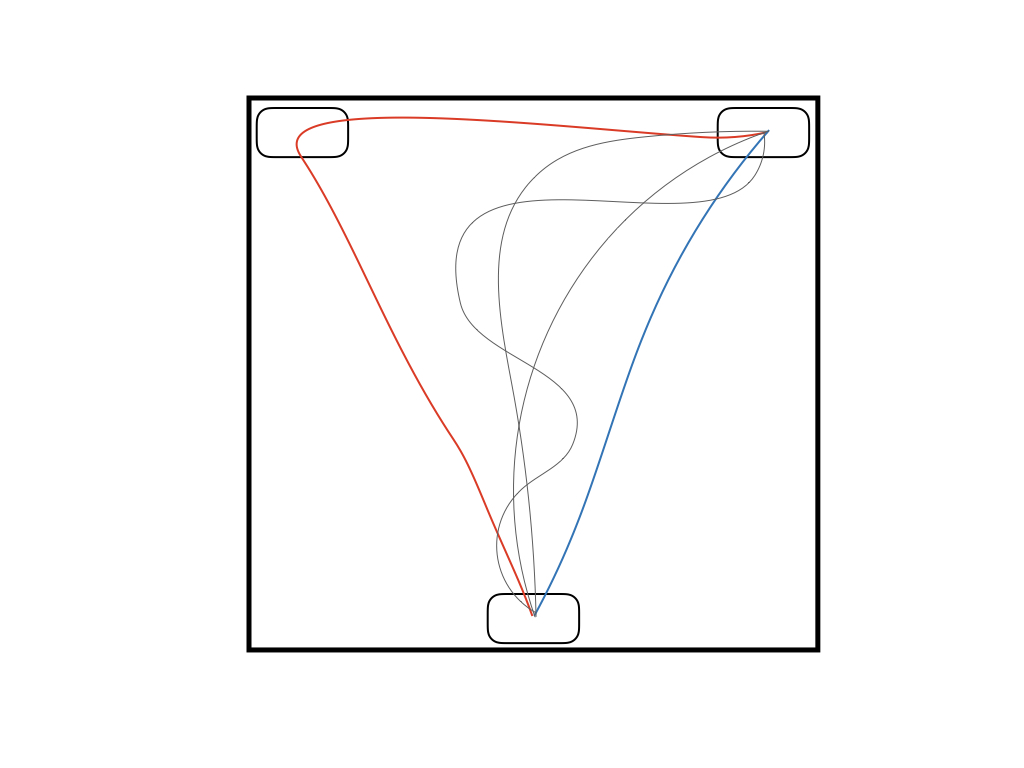
\includegraphics[width=\textwidth]{trajectories.jpeg}
\caption{Shape of trajectories underlying distinct decision processes. One single cognitive process is expected to be mapped onto one smooth movement (blue line), whereas a change of mind would be reflected by two movements (red line). Intermediate cases are represented in gray.} \label{fig:scheme.traj}
\end{figure}

Our main goal here is to test the connection between cognition (decision making) and action (mouse trajectories): Are decision processes always reflected in mouse trajectories? If yes, how are they reflected? 
One could easily imagine a situation where two different trajectory shapes do not correspond to two different decision mechanisms, but to a single one (due to uncertainty, noise, etc.). Differences in trajectories can therefore underlie something other than decision shift. 

In this paper, we address these questions by identifying the features in mouse-trajectories corresponding to two different types of decisions: \emph{straightforward} decisions (i.e. single commitment) and \emph{shifted} decisions (i.e. a change of mind). 
% developing a rule to dissociate mouse-trajectories... 
First, we present a \emph{validation} experiment where, instead of taking mouse trajectories as indicators of cognitive processes, we \emph{manipulate} whether or not our stimuli trigger a flip in decision (\Cref{section:validation}). 
The data from this validation experiment (i.e. two groups of `quasi-decisions') is then used to fed a \emph{linear discriminant analysis} (henceforth, LDA), trained to classify trajectories depending on the underlying decision (\Cref{section:LDA}). 
After comparing the performance of LDA classifier to other traditionally used mouse-tracking measures (\Cref{section:other-mt}), 
the LDA classifier will be further tested with new data, obtained from a replication of Dale and Duran's (\citeyear{Dale2011}) experiment on negation processing (\Cref{section:replication}). If there is a change of decision triggered by negation, trajectories corresponding to negative trials should be classified together with trajectories underlying decision change in the validation experiment. 


\section{Manipulating decision making: Validation Experiment}
\label{section:validation}

We developed an experiment where participants had to perform a \emph{two-alternatives forced task}: at each trial, they were presented with a colored frame surrounding the screen and they had to determinate whether the frame was blue or red. 
Responses were made by clicking on the ``blue" or ``red" buttons, allowing the recording of mouse-movements during each trial. Importantly, responses were considered accurate if they described the color at the moment of the click. 
In order to mirror decision processing, we manipulated whether the color of the frame remained stable or changed at some point during the trial. 
While in the latter case the initial choice will be the accurate response (\textit{straightforward} trials), in the former, participants were forced to swap their answer (\textit{switched} trials), mimicking a change of decision. Note that, since we are only \emph{mirroring} decision making, we refer to these decision processes as \emph{`quasi-decisions'}.   
An illustration of the procedure is provided in \Cref{fig:procedure.example}. 

%Participants were instructed to answer as fast as they can.


\begin{figure}
\centering
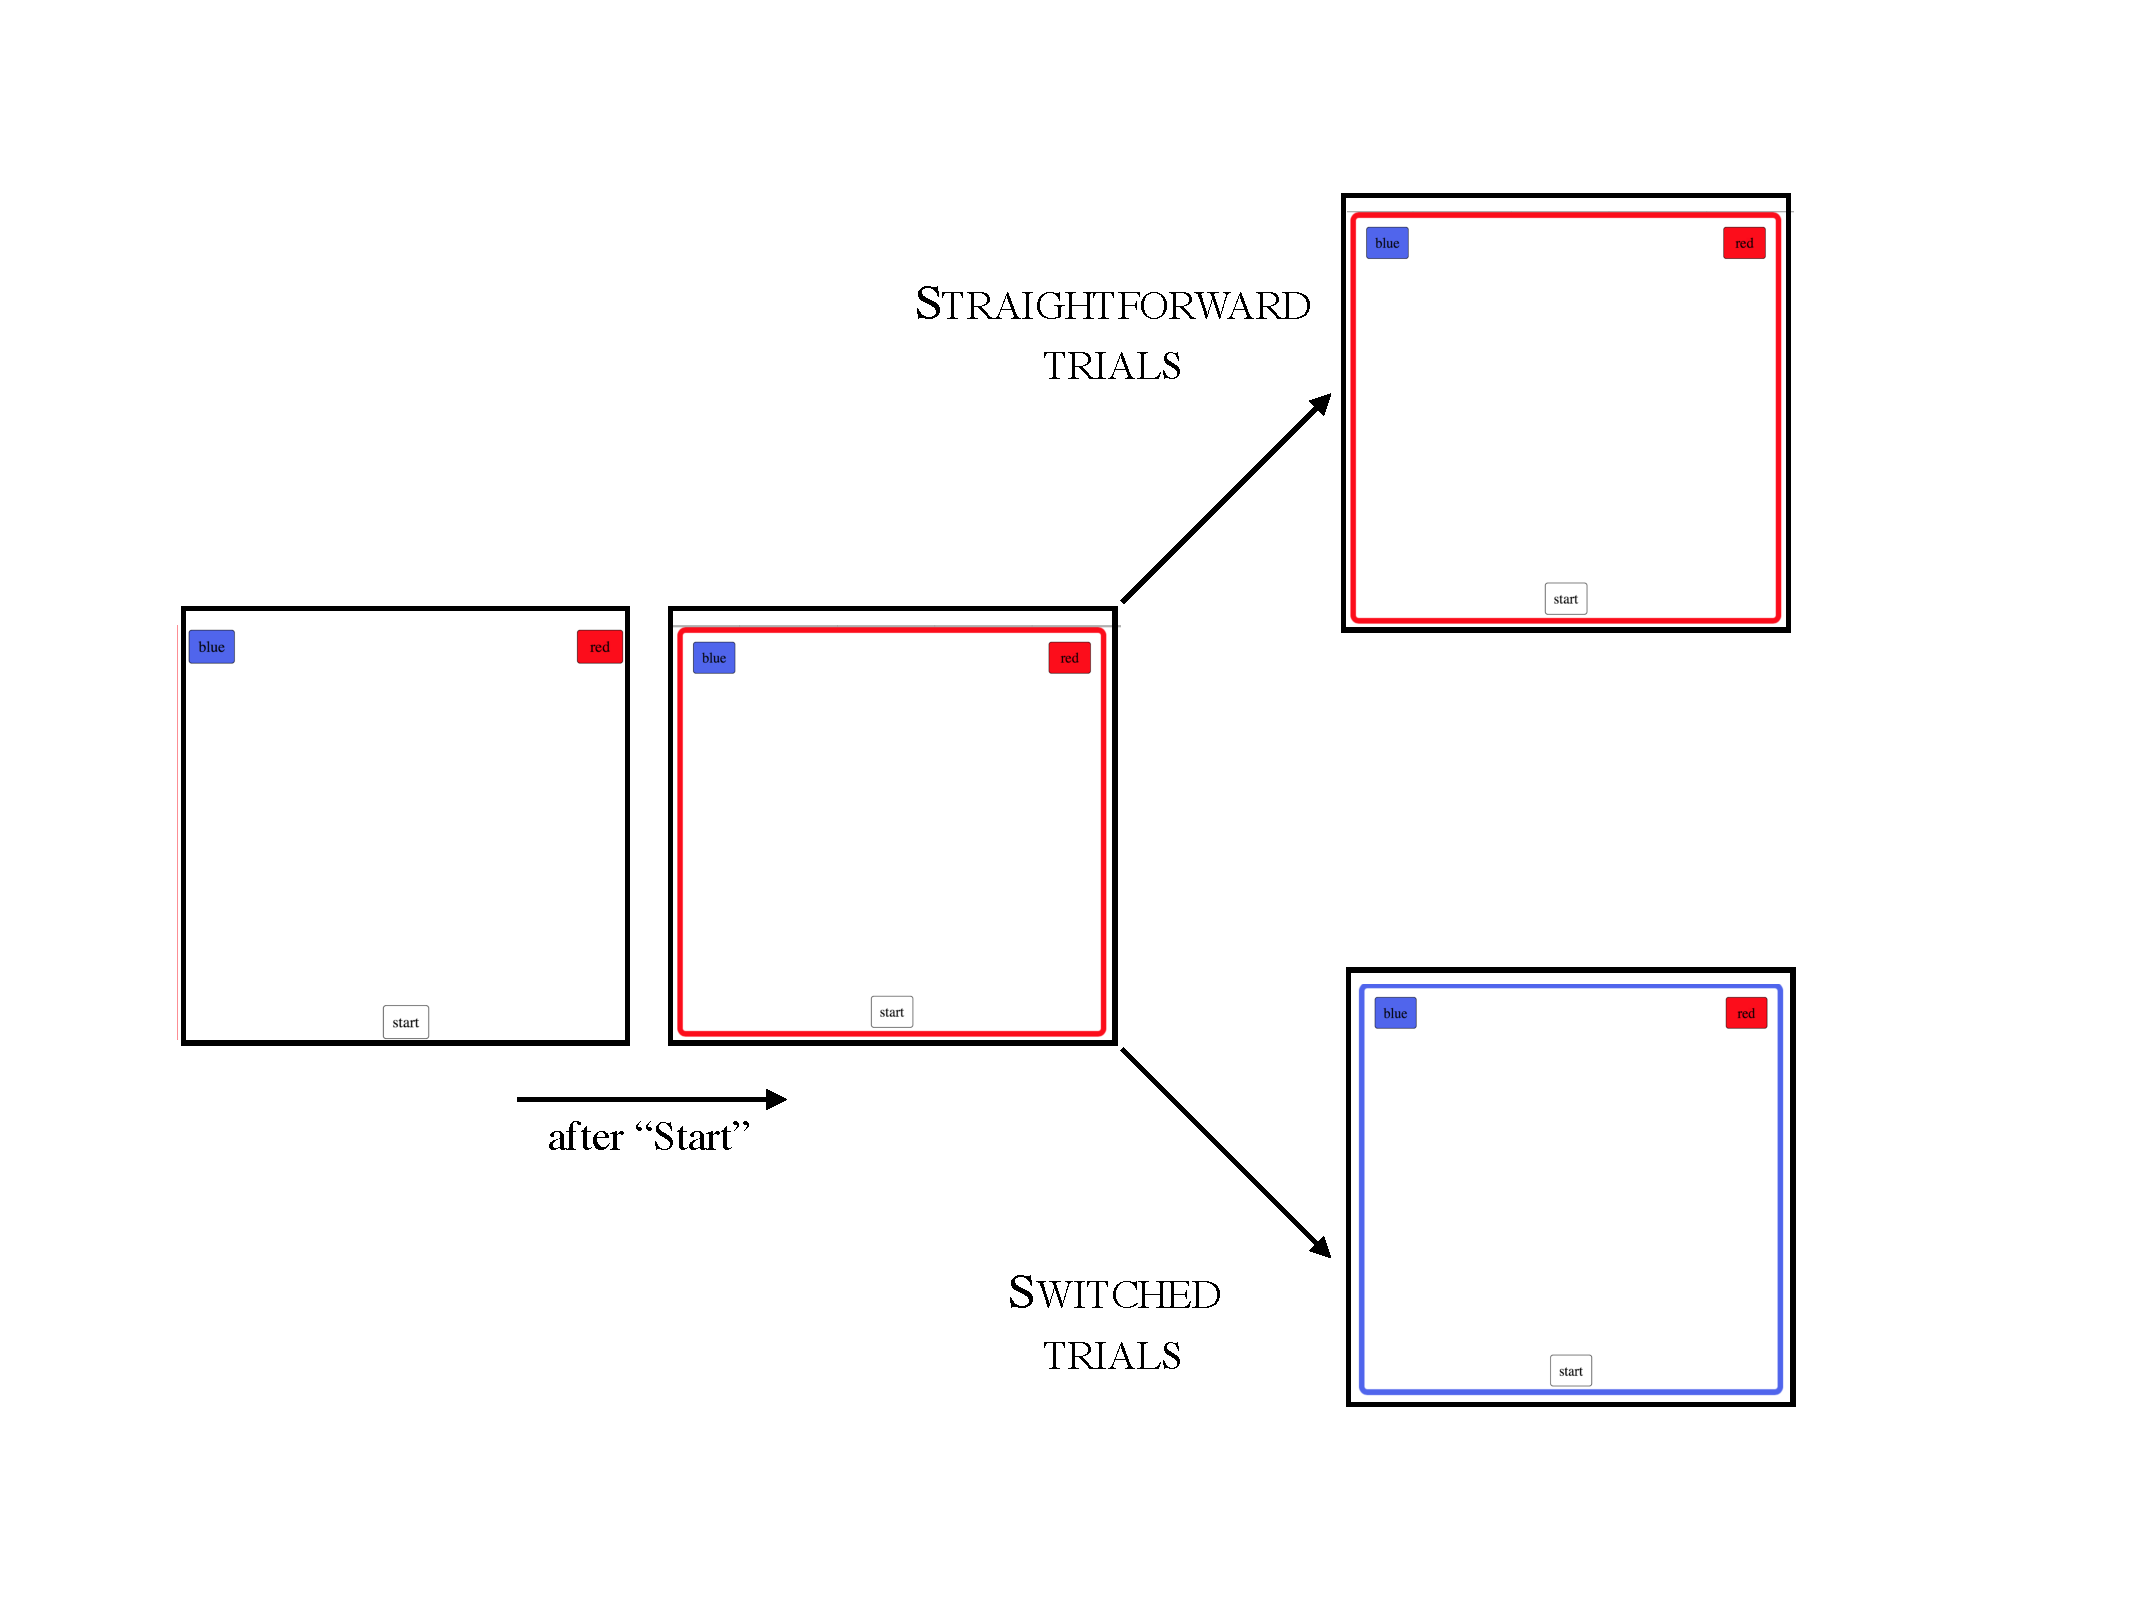
\includegraphics[scale=.5]{procedure.pdf}
\caption{\textbf{Procedure in Validation Experiment.} Subjects were instructed to click the `Start' button in order to see the colored frame. Response boxes were on the top-left or top-right. Depending on the trial condition, the frame color could change along the trial or not.} \label{fig:procedure.example}
\end{figure}

\paragraph{Participants} Fifty four participants (F=27) were recruited using Amazon Mechanical Turk. Two subjects were excluded from the analyses because they did not use a mouse to perform the experiment. All of them were compensated with 0.5 USD for their participation, which required approximately 5 minutes. 

\paragraph{Design}
Each trial instantiated one of two possible \textsc{Decision pattern}s. In \textit{straightforward} trials, the frame color remained stable, and the decision made at the beginning of the trial did not need to be revised. Conversely, in \textit{switched} trials, the color swapped during the trial, forcing a revision of the initial choice. 
The \textsc{point of change} in \textit{switched} trials was determined by the position in the \textit{y} axis, and it could be early, middle or late. 
The \textsc{Frame color} at the response point was also controlled: it could be red (right button) or blue (left button).    
A summary of the design is given in \Cref{tab:design.validation}. 


\begin{table}[!h]
\centering
\begin{tabular}{c|cc|c}
\textsc{Decision Pattern}&\multicolumn{2}{c|}{\textsc{Frame color}}&\textsc{Point of change}\\
\hline
\multirow{2}{*}{Straightforward} & \multicolumn{2}{c|}{Blue} & -- \\
& \multicolumn{2}{c|}{Red} & -- \\
\hline
\multirow{2}{*}{Switched} &Blue & Red & early (y=.4), middle (y=.7), late (y=.9) \\
 &  Red &  Blue & early (y=.4), middle (y=.7), late (y=.9) \\
\hline
\end{tabular}
\caption{Design in Validation Experiment}
\label{tab:design.validation}
\end{table}

To prevent participants from developing a strategy based on staying on the middle of the screen, the proportion of trials was adjusted so that straightforward trials were the majority (32 repetitions per frame color), whereas switched trials had 4 repetitions per frame color and change point. The total number of trials was 88.  

\paragraph{Interface}
The interface was programmed using JavaScript. Mouse movements triggered the extraction of $x,y$-pixel coordinates (i.e., no constant sample rate). The software was adapted proportionally to the window of the participant's browser, forming a rectangle: the height was covered at 100 percent and the width was 120 percent of the height. 
Three buttons were displayed during the experiment (`start' and response buttons). Their size was also determined by the browser window (i.e., approximately 20 percent of the total width). The `start' button was placed at the bottom center of the screen. The two response boxes were located at the top left (`blue') and top right (`red') corners of window. This location was constant across participants, and handedness was controlled.  
In each trial, mouse movements were recorded between start-clicks and response-clicks. The $x,y$-pixel trajectory was saved together with its raw time. Afterwards, the positions were normalised according to participants' window size, to allow comparisons between subjects. The normalization was done by considering the start button at the [0,0] point, the `blue' button corner at [-1,1] and the `red' button at [1,1]. 

\paragraph{Data treatment}
Mouse-tracking data are particularly variable trial to trial. On one hand, variations in response times imply different quantity of \textit{x,y} positions per trial, making difficult the comparisons between items. On the other hand, in our design, positions are extracted based on mouse movements, and devices with more or less sensibility could influence the number of samples taken during the trial. In order to compare mouse trajectories, we normalized the time course into 101 proportional times steps (percentage of trial duration). This normalization, as all the other calculations, was performed in the Spyder environment using Python 2.7. 

\paragraph{Overall performance}
Inaccurate responses, corresponding to 4\% of the data, were removed from the analyses. 
Mean trajectories for each \textsc{decision type} and \textsc{decision point} are illustrated in \Cref{fig:mean.trajectories.calibration}. 
%Temporal information about changes in the $x$ coordinate is provided in the appendix (Figure X). 
These trajectories suggest that participants made a decision as soon as they were presented with the color frame, and revised this decision if needed. When they were forced to change their choice, this switch was reflected in mouse trajectories. 
\addMM{MM: Do we want to include other graphs?}

\begin{figure}
\centering
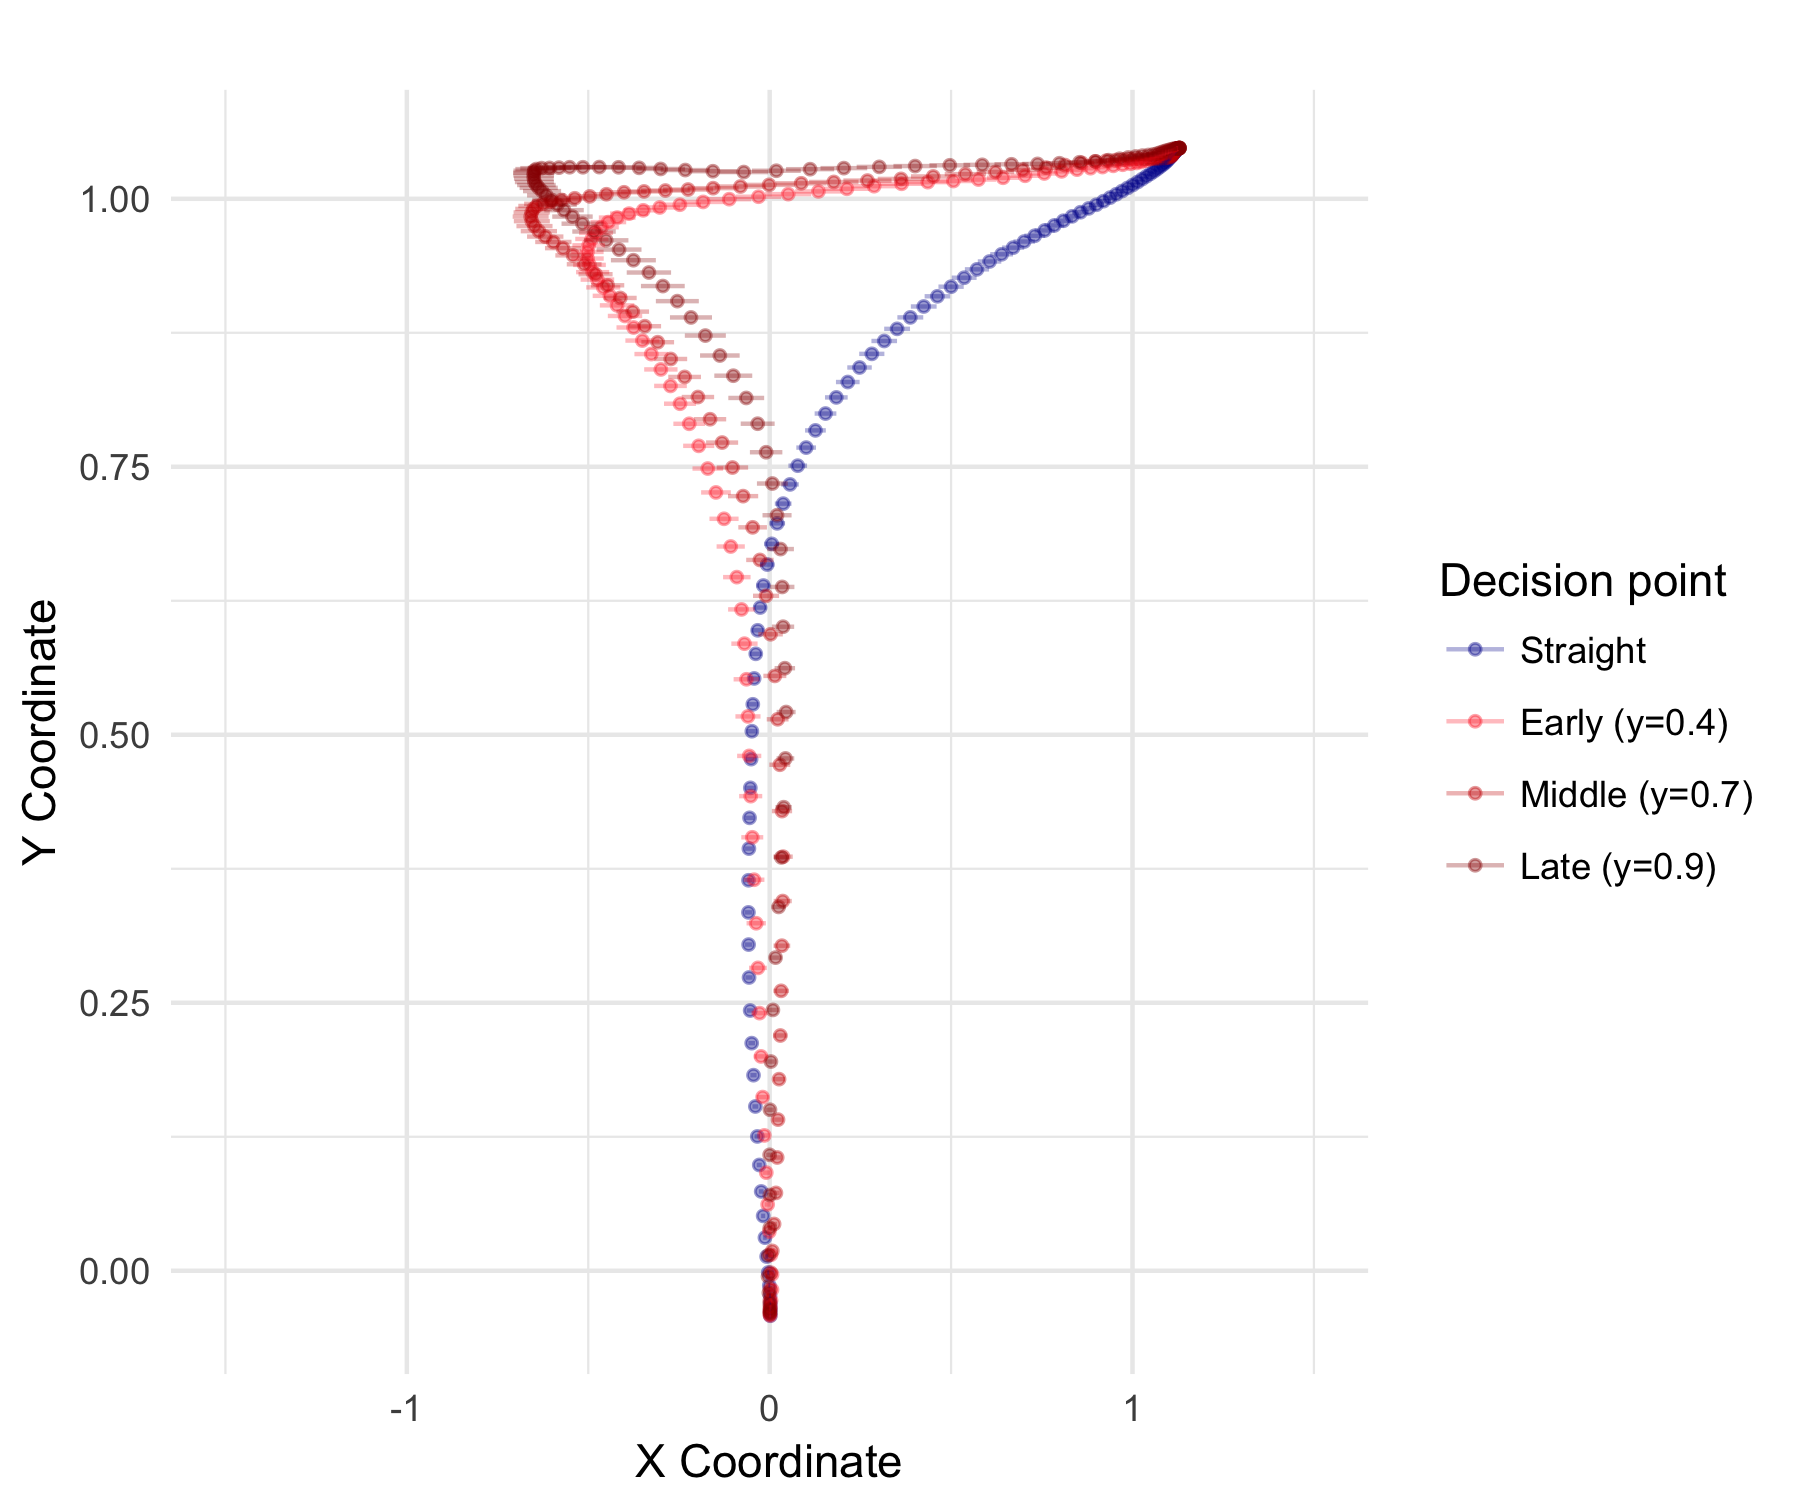
\includegraphics[width=\textwidth]{calibration_mean_trajectory_pointchang.png}
\caption{Mean trajectories per class}\label{fig:mean.trajectories.calibration}
\end{figure}

\section{Classifying decision processes with LDA}
\label{section:LDA}
Different `quasi-decisions' (i.e. \textsc{Decision pattern}s) have a different impact on mouse trajectories, as observed in \Cref{fig:mean.trajectories.calibration}. To identify the features characteristic of each class (\textit{switched} vs. \textit{straightforward}), we use a Linear Discriminant Analysis method for classification. 

\paragraph{Description of LDA classifier}
The LDA is an optimal solution to classify continuous data --such as trajectories-- into two or more classes --such as decision patterns (straightforward vs. switched quasi-decisions). In a nutshell, the LDA algorithm assumes that different classes have a common covariance matrix, and finds the linear combination of predictors that gives maximum separation between the classes. This linear combination of predictors is obtained as a linear coefficient and it can be used to form a decision rule for the classification.  It is a single number that represents the position  on a line running between the two classes that maximizes their separability, with zero representing the midpoint between the two.
 
The predictors used by the classification algorithm were: (a) the \textit{x,y} coordinates, (b) Euclidean-based velocity, and (c) Euclidean-based acceleration (both of which are non-linear with respect to the original $x,y$ coourdinates). The coordinates provide absolute spatio-temporal information about where the cursor was when, and velocity and acceleration provide information about how did it arrived there.
To avoid collinearity (which causes problems for LDA), we applied a Principle Component Analysis (PCA) to identify the 13 principal components on these predictors, and performed the LDA on these principal components. 
We thus obtained an \emph{LDA measure} for each trial, the single number giving the position of the trial on the LDA classification  axis.
A diagram of the procedure is provided in \Cref{fig:diagram}.

\begin{figure}

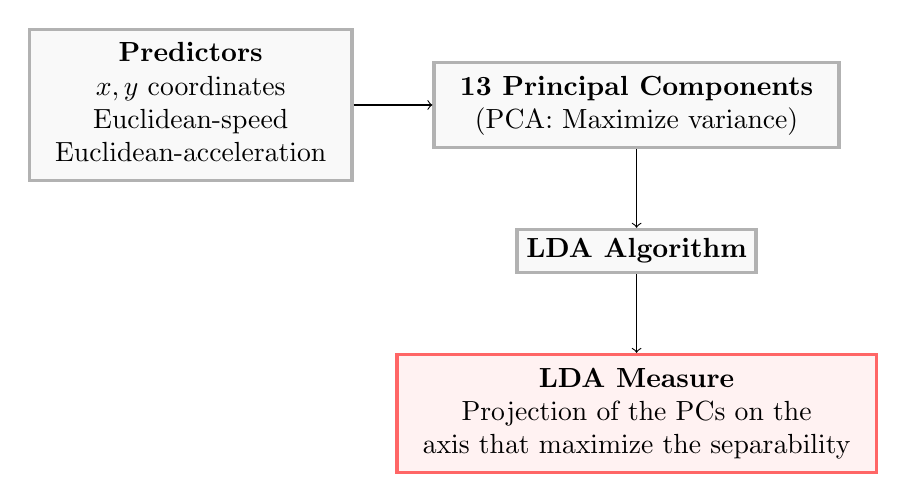
\begin{tikzpicture}[
squarednode/.style={rectangle, draw=gray!60, fill=gray!5, very thick, minimum size=5mm},
squarednode2/.style={rectangle, draw=red!60, fill=red!5, very thick, minimum size=5mm},
]
%Nodes
\node[squarednode]      (pca)                              {\begin{tabular}{c} \textbf{13 Principal Components} \\ (PCA: Maximize variance)\end{tabular}};
\node[squarednode]        (pred)       [left=of pca] {\begin{tabular}{c} \textbf{Predictors} \\ $x,y$ coordinates \\ Euclidean-speed \\ Euclidean-acceleration \end{tabular}};
\node[squarednode]      (lda)       [below=of pca] {\textbf{LDA Algorithm}};
\node[squarednode2]        (ldameasure)       [below=of lda] {\begin{tabular}{c} \textbf{LDA Measure}\\ Projection of the PCs on the \\ axis that maximize the separability  \end{tabular}};
 
%Lines
\draw[->] (pred.east) -- (pca.west);
\draw[->] (pca.south) -- (lda.north);
\draw[->] (lda.south) -- (ldameasure.north);


\end{tikzpicture}
\caption{Diagram}\label{fig:diagram}
\end{figure}

\paragraph{Performance of the LDA classifier}
The result of applying the procedure described in \Cref{fig:diagram} to the trajectories in the validation experiment is illustrated in \Cref{DIST:LDA}. 
To evaluate the overall performance of the classifier, we calculated the area under the ROC curve (AUC), a standard method for evaluating classifiers \citep{Hastie}. Intuitively, the AUC gives the degree to which the histograms resulting from the classifier's continuous output (for example, \Cref{DIST:LDA}) is non-overlapping in the correct direction (in this case, ``switched'' more systematically in the positive direction on the classification axis than ``straightforward''). 


\begin{figure}
\centering
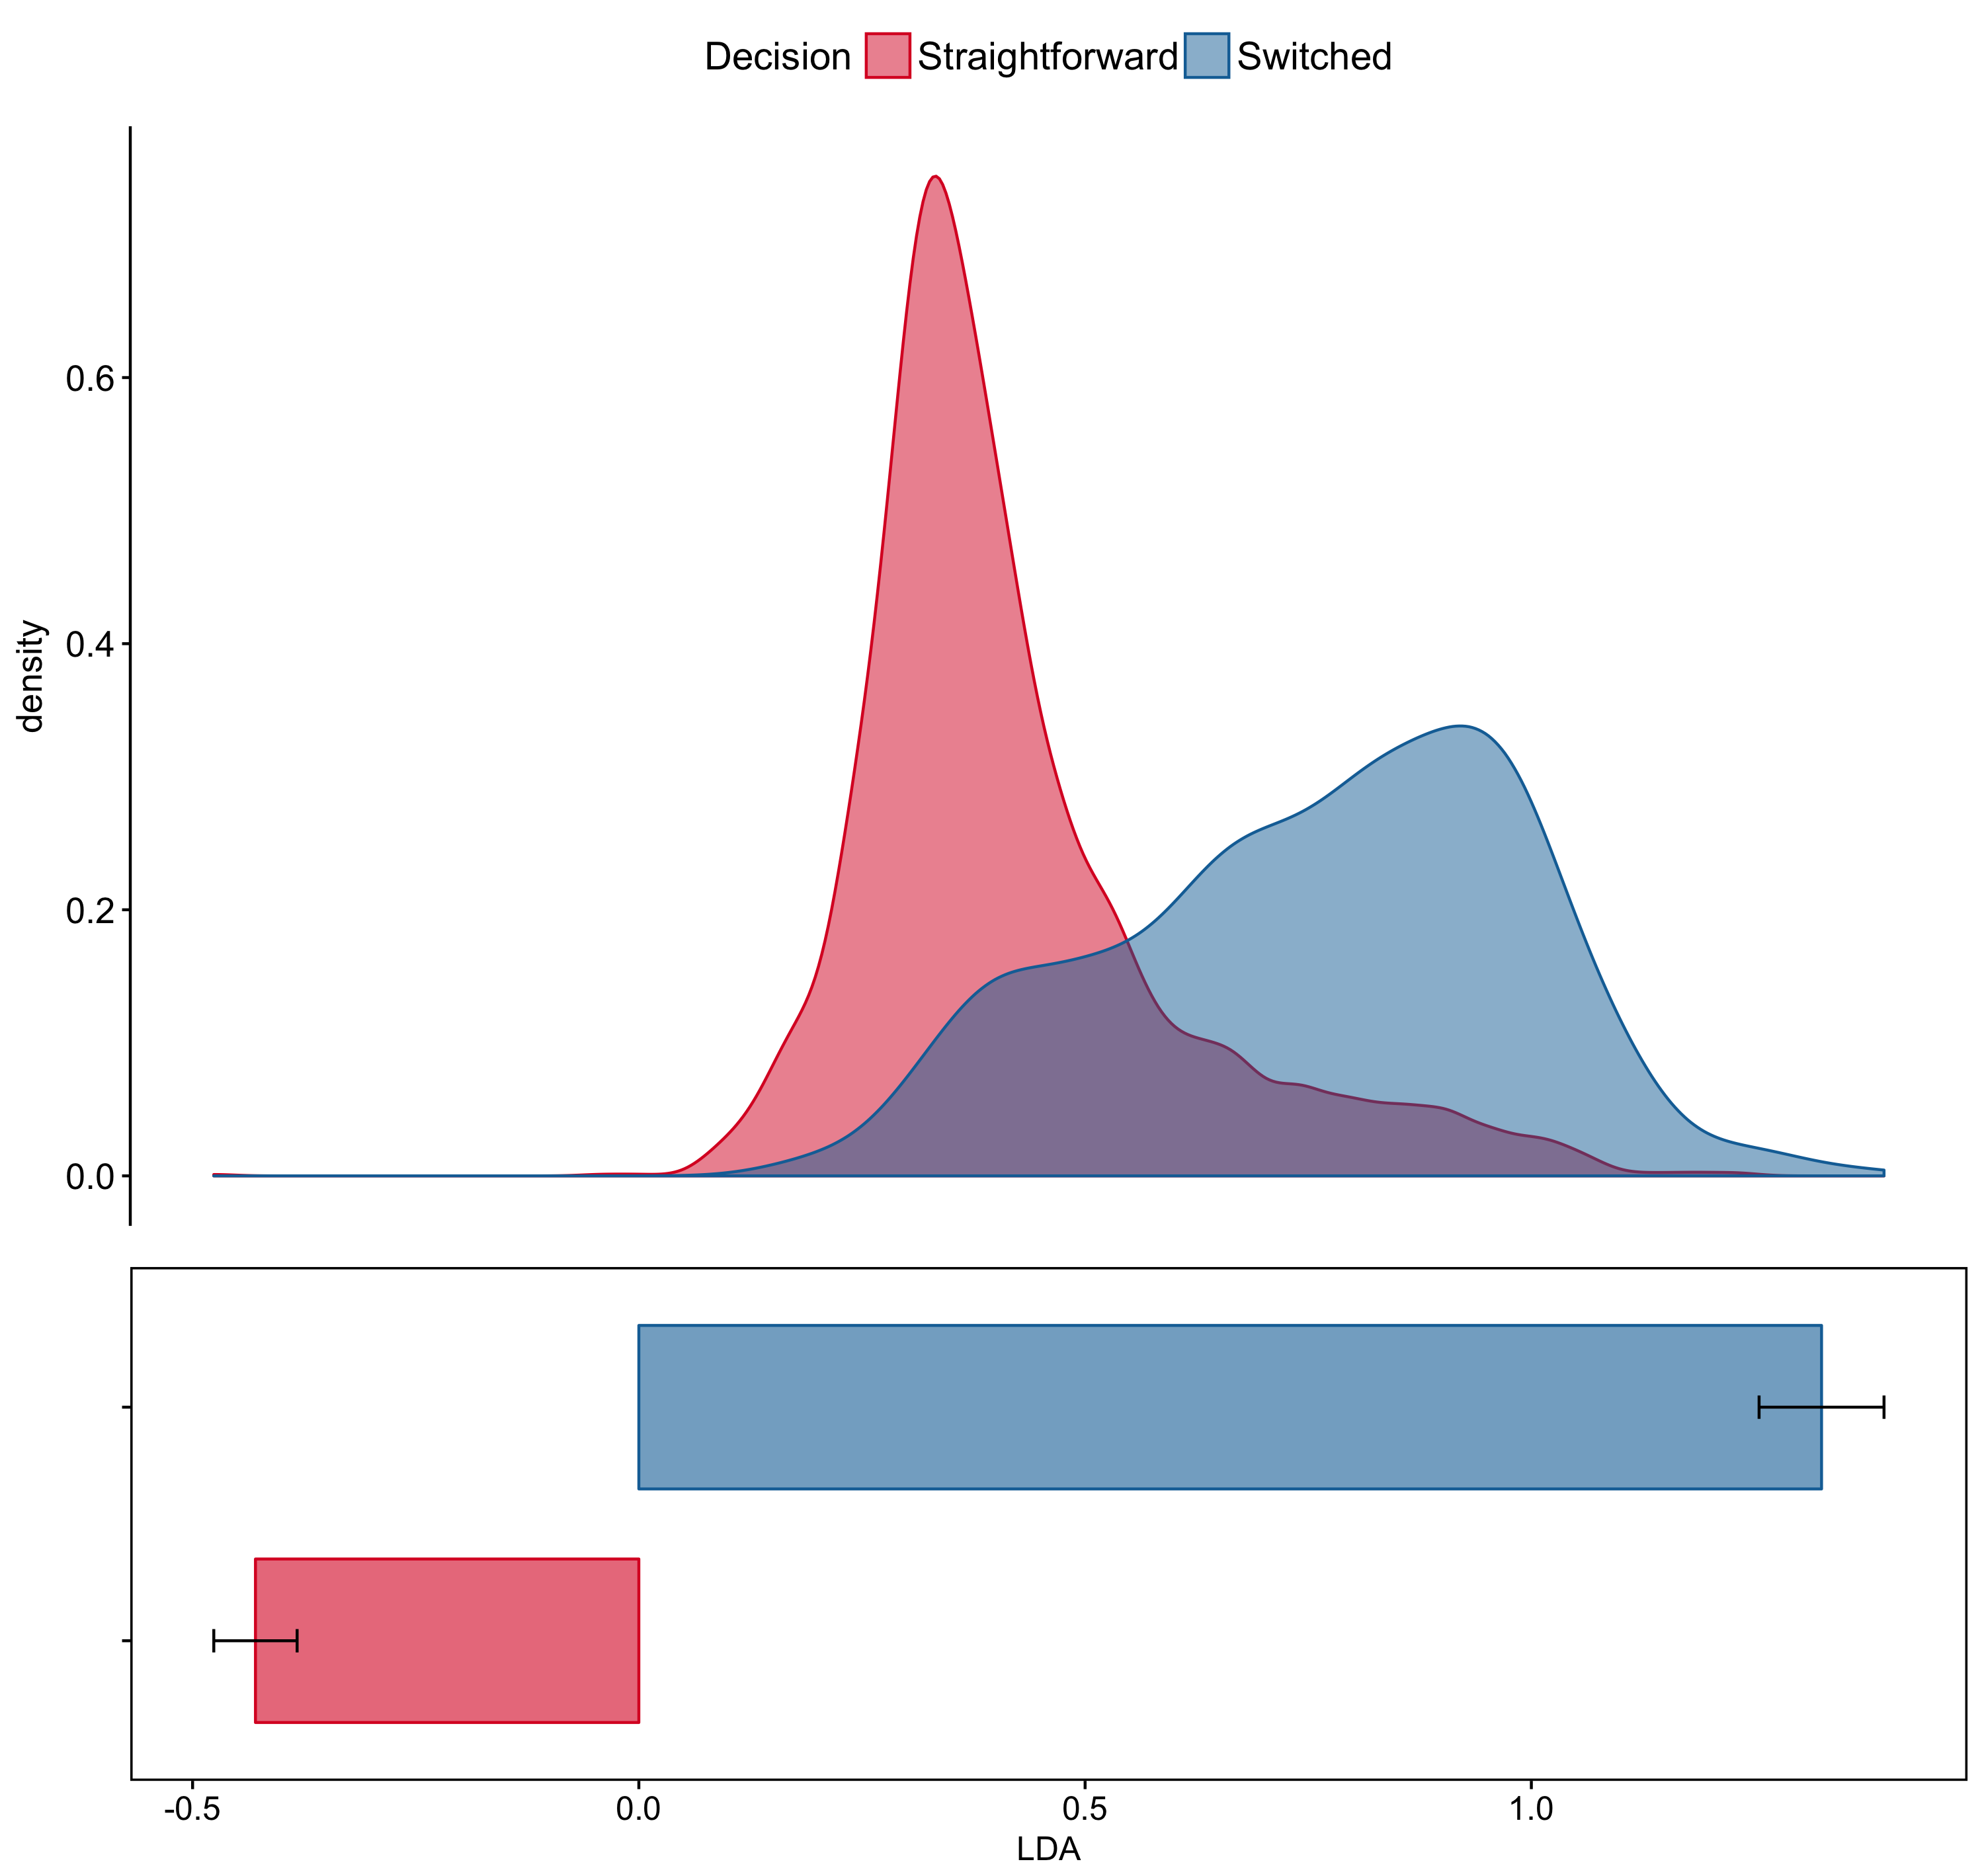
\includegraphics[width=\textwidth]{lda_distribution_calibration.png}
\caption{Classifier performance} \label{DIST:LDA}
\end{figure}

To properly evaluate the classifier's perfomance at separating trials following the distribution in the experiments, the AUC measure was cross-validated. That is, calibration data were partitioned into 10 bins that kept the proportion of \textit{straightforward} and \textit{switched} trajectories constant (75/25 proportion). For each bin, we took the complementary set of data (the rest 90\%) to train the classifier. The data contained in the bin were used as test set to diagnose the classifier performance. Thus, we obtained one AUC score for each test bin (ten bins). The performance of the LDA classifier was compared to \emph{baseline}, equivalent the worst possible outcome, and a \emph{topline}, which was what we would expect from the classifier under the best possible conditions. 
For the baseline, we used a random classifier that assigned labels by sampling from a beta distribution centred at the probability of straightforward trials; the topline was computed by testing and training the original LDA classifier with the same set of data. 
The mean AUC values for the LDA, the baseline and the topline in each bin are given in \Cref{DIST:AUC}a. 

To assess whether the performance of the LDA classifier was statistically different from baseline (or topline performance), we tested how likely it would be to obtain the attested differences under the null hypothesis that the LDA classifier performance was the same as the baseline (or topline) performance.   
The difference in AUC means between each pair of these two pairs of classifiers was calculated, and the sampling distribution under the null hypothesis was estimated by randomly shuffling the labels indicating which classifier the score came from.

In \Cref{table:comparisons.permutation.1}a, we report the results of performing a one-tail test on these mean differences (observed vs. under null hypothesis). As expected, our original LDA is significantly better than a random classifier at categorising trajectories into the two classes. Conversely, there is no significant difference between the performance of our LDA and the topline (i.e., the LDA is not significantly different from the best possible classification). 

\begin{figure}
\centering
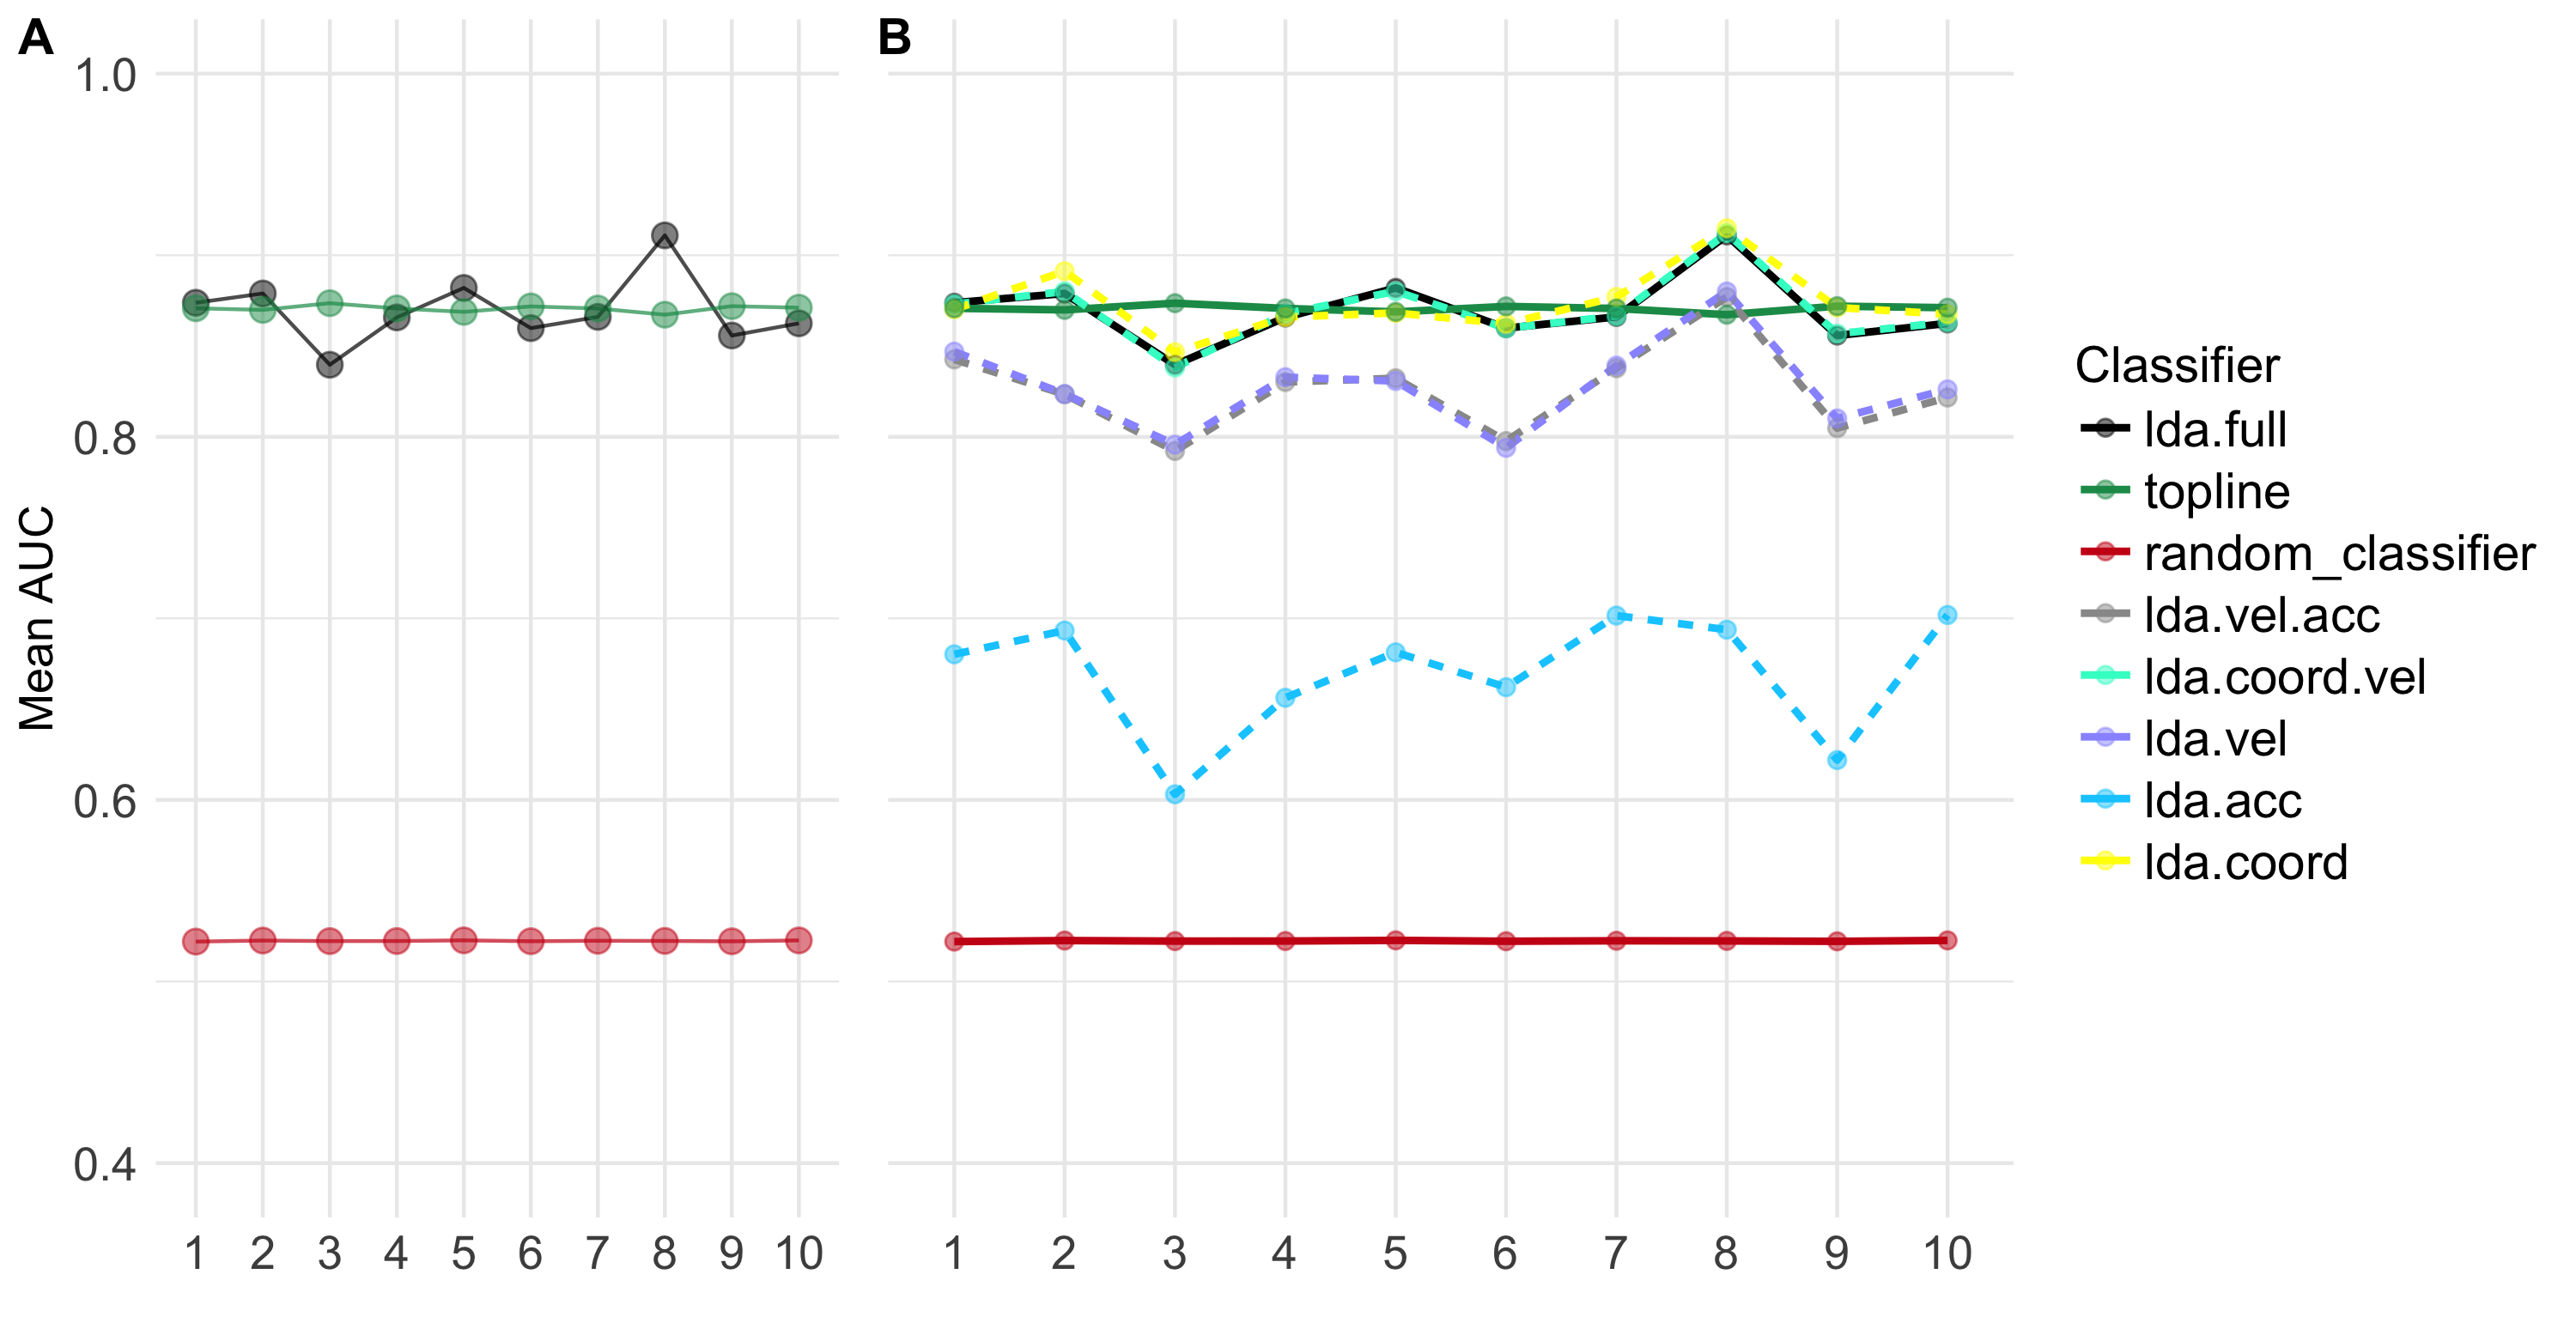
\includegraphics[width=\textwidth]{auc_calibration_2.png}
\caption{Mean AUC values} \label{DIST:AUC}
\end{figure}


\begin{table}[h]
\centering
{\footnotesize
\begin{tabular}{p{1.5cm}>{\columncolor[gray]{0.8}}p{1.5cm}cc|p{1cm}cccc}

 \multicolumn{2}{c}{ } &  \multicolumn{2}{c}{(a)} & \multicolumn{4}{c}{(b)}\\
\hline
& \centering \textsc{Original LDA}& \multirow{2}{1.1cm}{\centering \textsc{Baseline}} & \multirow{2}{1.1cm}{\textsc{Topline}} &\multicolumn{5}{c}{\textsc{LDA with different predictors}}\\
\cline{5-9}
& \centering (coords, speed, acc) &  & & \centering coords, vel & vel, acc & coords & vel & acc \\[0.5cm]

\hline
\centering \textbf{AUC (mean)} & \centering .87& .52 & .87 &\centering .87 & .83 & .87 & .82 & .67 \\[0.5cm]
%& .88 & .84  \\[0.5cm]
\hline
\centering \textbf{Mean \\ Difference} & \centering -- & .35 & -.002 &\centering -.0004 &  .04 & -.006 & .04 & .2 \\[0.5cm]

%& -.006 & .05   \\[0.5cm]

\hline
\centering \textbf{$p$ value} & \centering  --  &  $<$.001 & 0.58 & \centering .5 & $<$.001 & .68 & $<$.001 & $<$.001 \\
%& .72 & $<$.001 \\
\hline
\end{tabular}}
\caption{Cross-validation results for the LDA classifier. The performance of the LDA was compared to the one of (a) Random and Topline classifiers and (b) LDA classifiers with different predictors.}
\label{table:comparisons.permutation.1}
\end{table}

\paragraph{Meaningful features and optimal predictors}
Our original LDA classifier takes as predictors both absolute and relative spatio-temporal features (coordinates, speed and acceleration).
Some of these features, however, might not be relevant for the classification. 
By comparing classifiers trained with different predictors, we can gather information about which features of mouse trajectories are more relevant for the distinction between decision processes (i.e. for the classification). 

We trained five additional LDA classifiers obtained by subsetting the three original LDA predictors. If both absolute and relative features are required to predict the decision type, we would expect our ``full'' original LDA classifier to be better than any other classifier that takes only a subset of these original predictors. 
The performance of these additional classifiers was diagnosed in the same way as before, by computing the AUC for each of the 10 test bins. \Cref{DIST:AUC}b illustrates the mean AUC values for each of these classifiers, together with the original LDA, the baseline and topline. 
Pair-wise comparisons with the original LDA were done by testing whether the observed mean differences would be expected under the null hypothesis (i.e. no difference in performance between classifiers). \Cref{table:comparisons.permutation.1}b summarises the comparisons between each of these classifiers and our original LDA. 	

The original LDA does not significantly differ from classifiers that contain the coordinates among their predictors, suggesting that the distinction between \emph{straightforward} and \emph{switched} `quasi-decisions' might be solely explained by the information contained in the $x,y$ coordinates. 
In contrast, the original LDA is significantly better than classifiers that use only speed and acceleration as predictors. These comparisons therefore reveal that, for classifying our validation data, absolute spatio-temporal features ($x,y$ coordinates) are generally better predictors than relative features (speed and acceleration). That is to say, it seems to be more relevant to know where are you when than how you got there. 

We caution that effects of true decisions, rather than the simulated quasi-decisions tested here, may indeed have an impact on speed and acceleration. It has been suggested that the speed and acceleration components can capture the level of commitment towards the response, such that a change of decision (\textit{swiched} trajectories) might have associated a specific speed/acceleration pattern \citep{Hehman2014}. This is not visible, however, in our data.


\section{LDA \emph{versus} traditional mouse-tracking analyses}
\label{section:other-mt}
The LDA classifier derives a solution to separating two kinds of mouse trajectories that is in a certain sense optimal. Previous studies have used alternative techniques to analyse mouse trajectories. In what follows, we will compare the performance of our LDA classifier to the one of other measures commonly used in mouse tracking studies. We focus on measures that mainly assess the spatial disorder in trajectories, which is typically taken to be indicative of unpredictability and complexity in response dynamics \citep{Hehman2014}.

Two of the most commonly used methods of mouse tracking \textbf{spatial analysis} are the \textit{Area under the trajectory} and the \textit{Maximal deviation} (henceforth, AUT and MD respectively) (see \citealp{Freeman2010})
The AUT is the geometric area between the observed mouse-trajectory and an idealised straight-line trajectory drawn from the start to the end points, whereas the MD is the point that maximises the perpendicular distance between this ideal trajectory and the observed path
(\Cref{fig:traditional-measures}). For both measures, higher values are associated with higher deviation peaks towards the alternative; values closer to zero (or below) suggest trajectory close to ideal. 
Another frequently used measure to estimate the complexity of the trajectory is based on quantifying the number of times the trajectories goes back and forth along the x-axis (horizontal flips, \citealp{Dale2011}, as illustrated in \Cref{fig:traditional-measures}).




\begin{figure}
\centering
\begin{subfigure}[b]{0.3\textwidth}
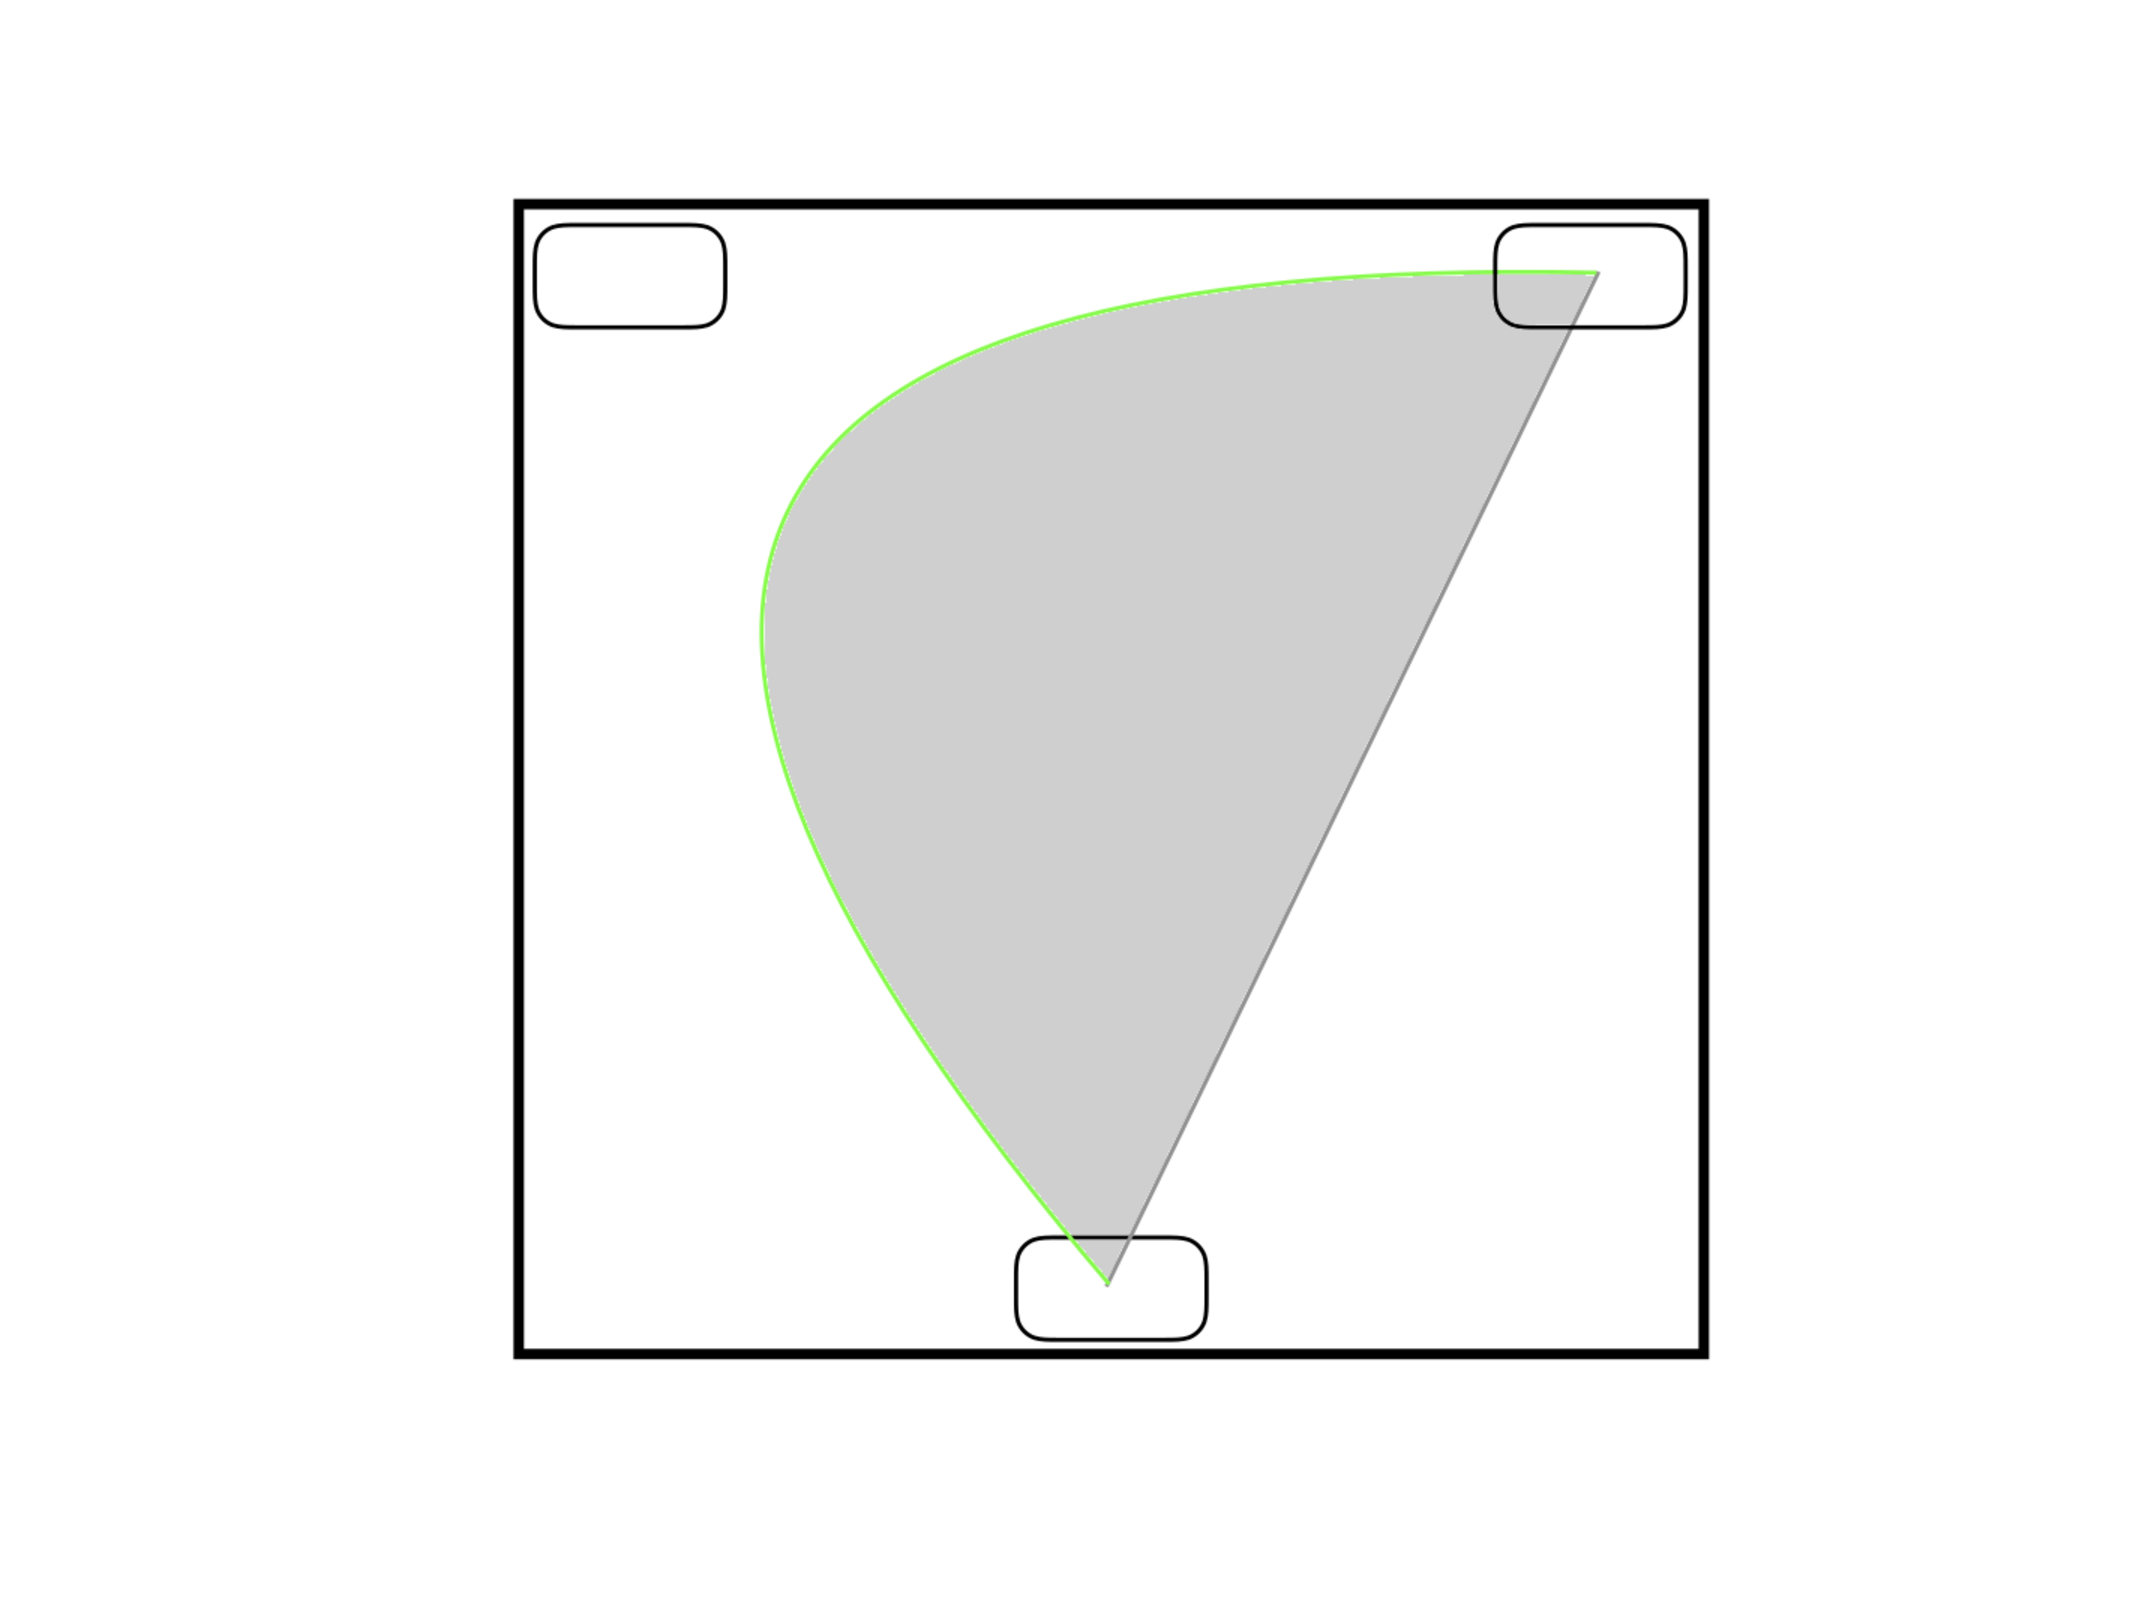
\includegraphics[width=\textwidth]{AUC.pdf}
\caption{Area Under the Trajectory}
\end{subfigure}
%
\begin{subfigure}[b]{0.3\textwidth}
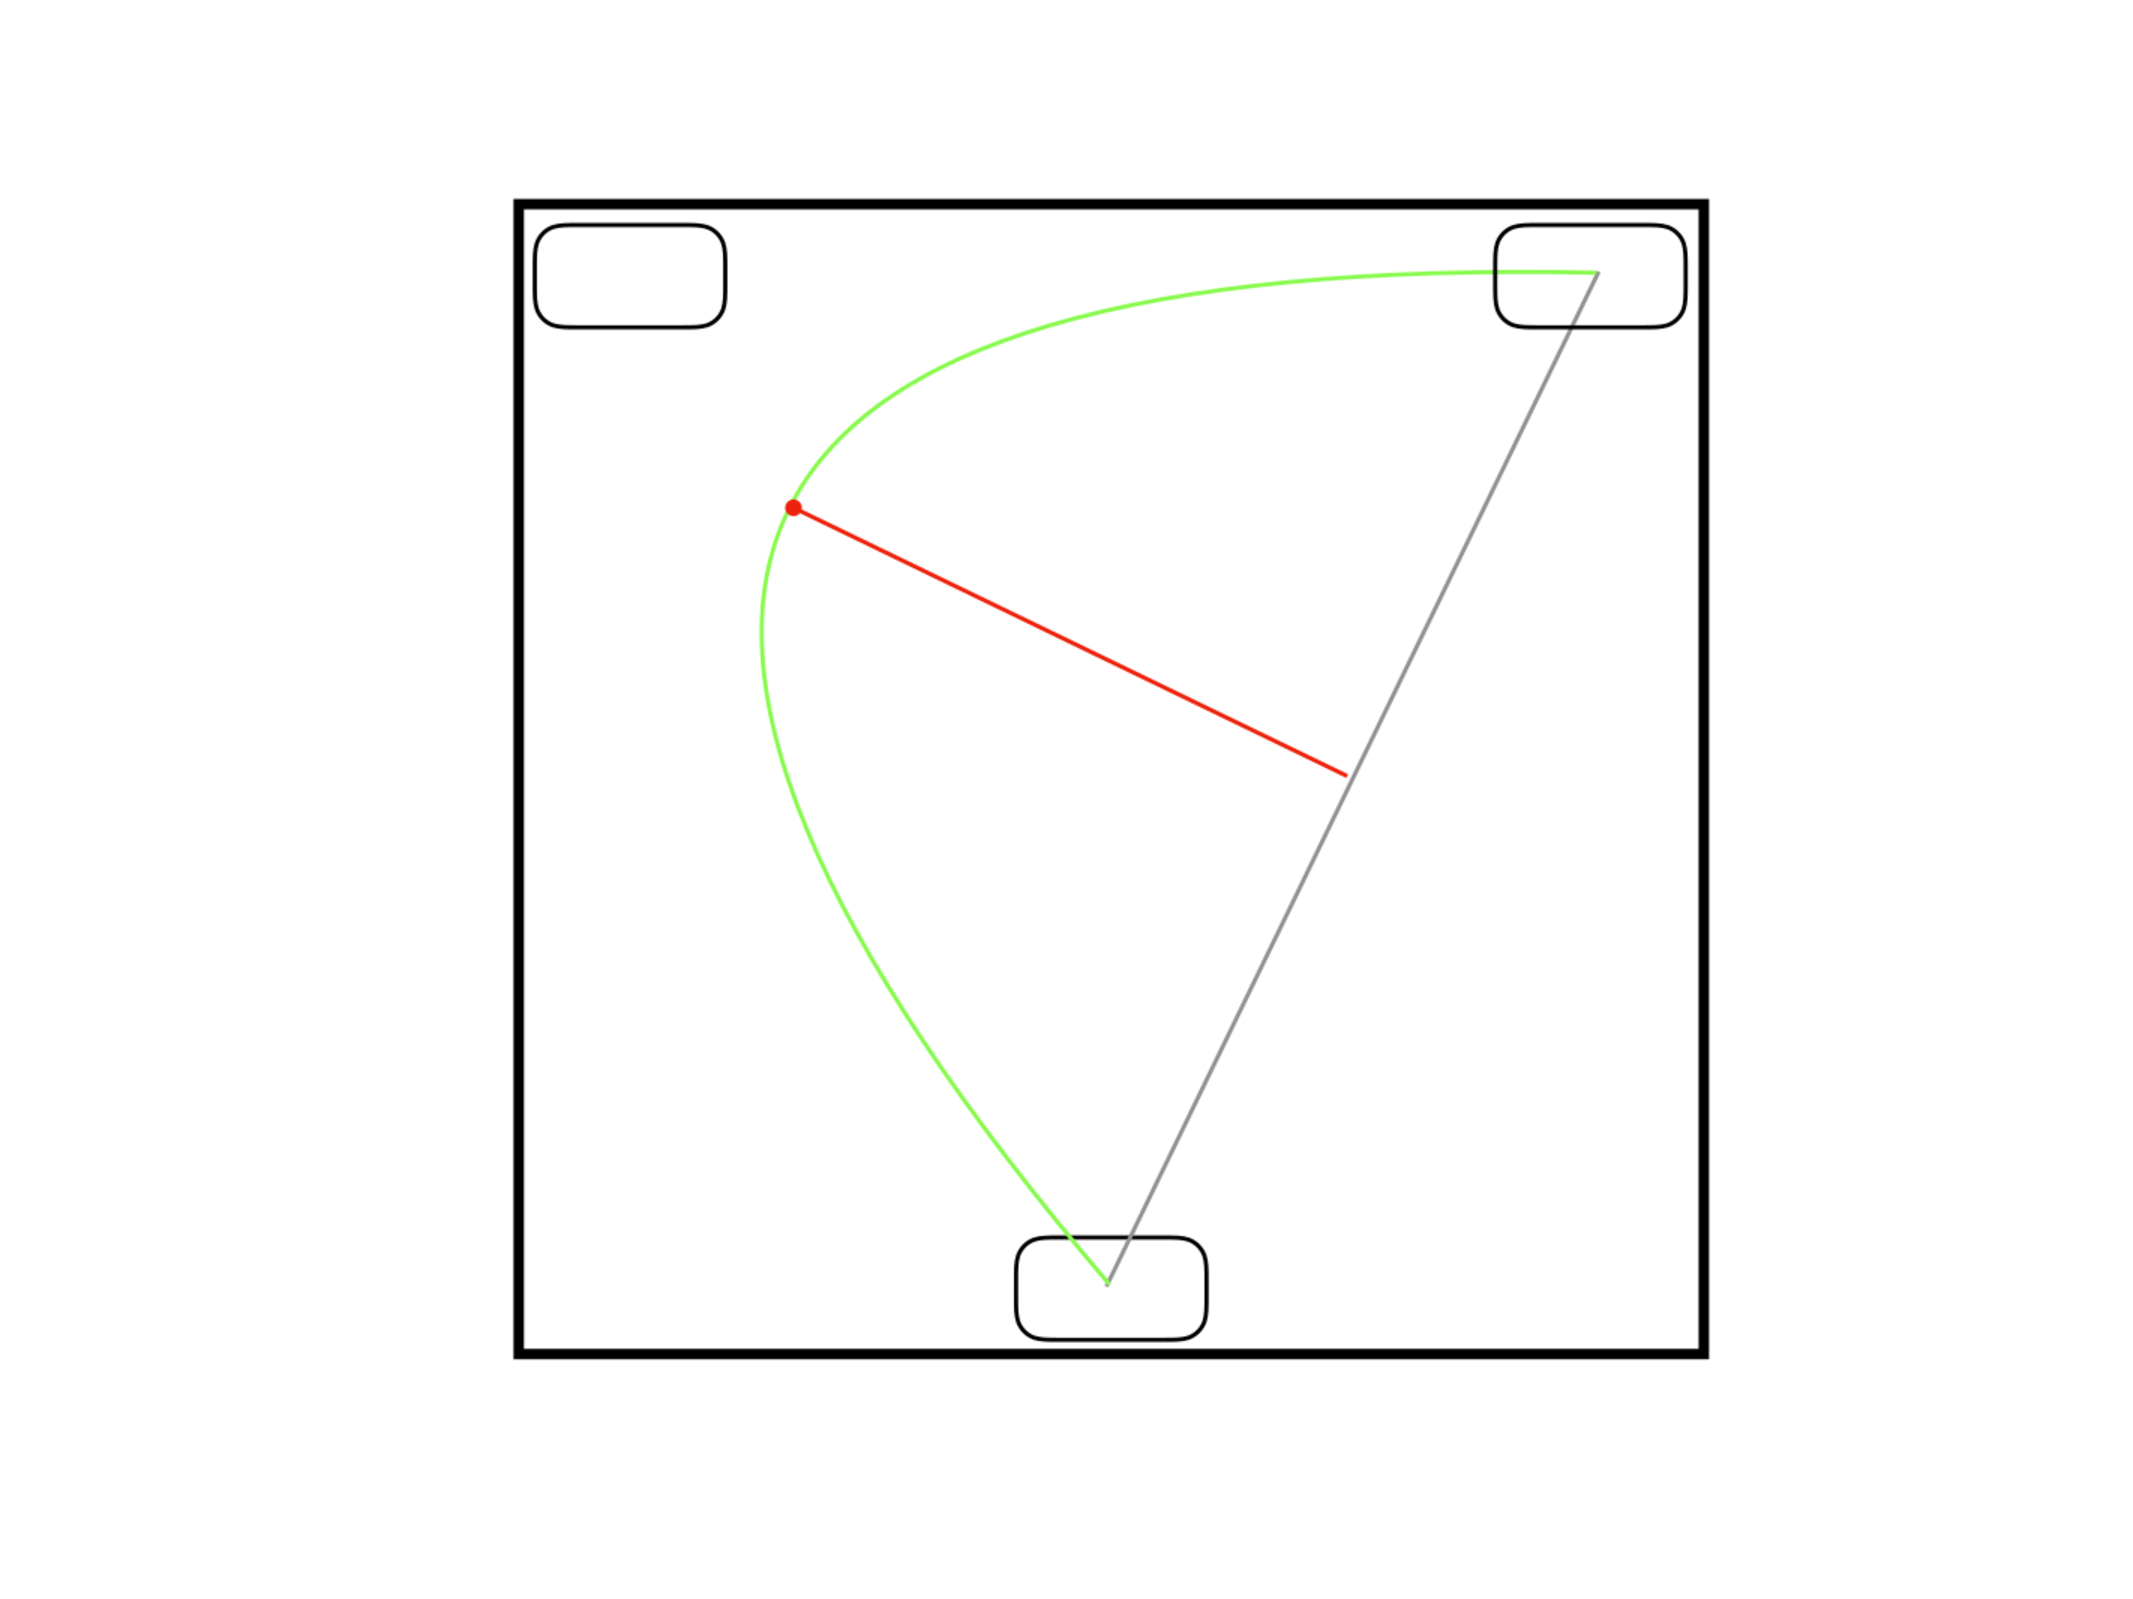
\includegraphics[width=\textwidth]{MD.pdf}
\caption{Maximal Deviation}
\end{subfigure}
%
\begin{subfigure}[b]{0.3\textwidth}
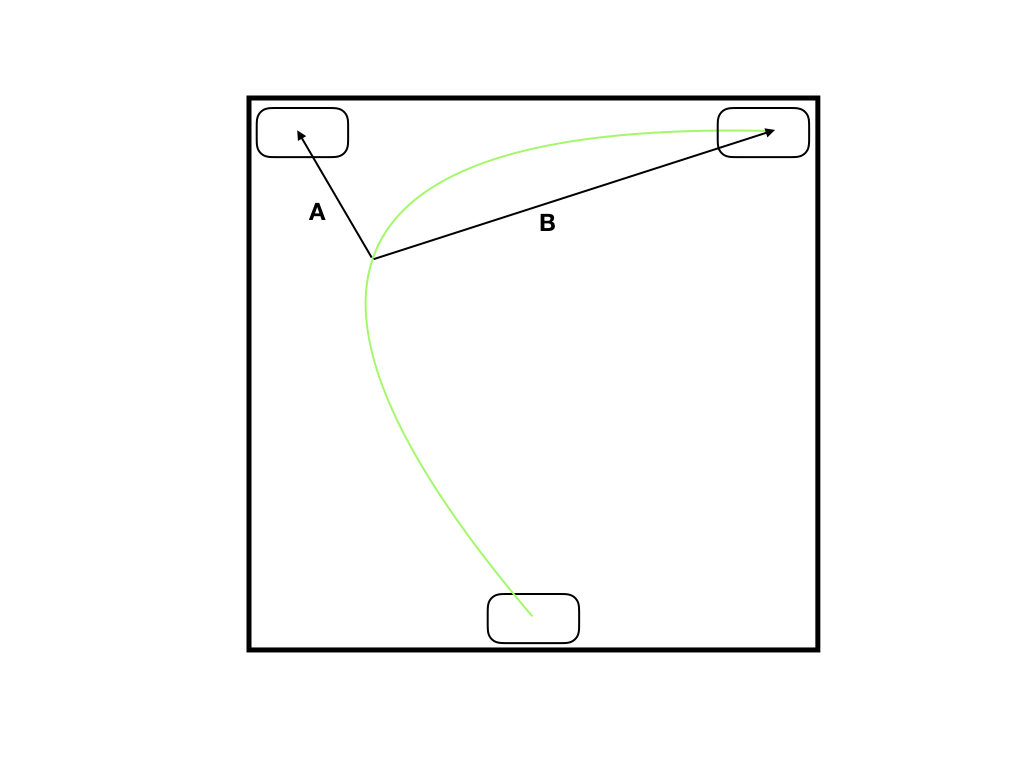
\includegraphics[width=\textwidth]{MaxRatio.jpeg}
\caption{Maximal LogRatio}
\end{subfigure}
\vspace{.5cm}

\begin{subfigure}[b]{0.45\textwidth}
%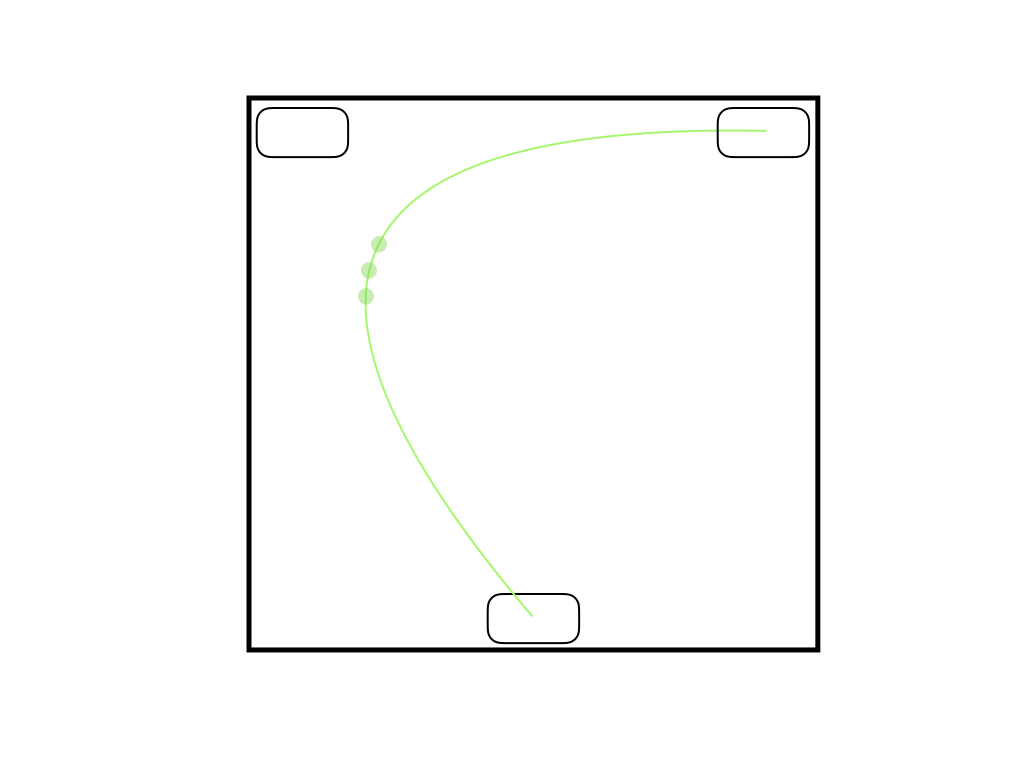
\includegraphics[width=\textwidth]{XFlips.jpeg}
\caption{X-coordinates Flips}
\centering
\(\sum H[(x_{t} - x_{t-1})(x_{t-1} - x_{t-2})] \)
\end{subfigure}
%
\begin{subfigure}[b]{0.45\textwidth}
\caption{Acceleration flips}
\centering
\((\sum H[( a_{t} - a_{t-1})( a_{t-1} - a_{t-2})])-1 \)

\end{subfigure}

\caption{Traditional mouse-tracking measures.}
\label{fig:traditional-measures}

\end{figure}



While all these measures serve to evaluate the degree of complexity of the path, they might fail to distinguish between `two-step' and `uncertain' decision processes --i.e., trajectories with a true deviation to the alternative or centred on the middle of the screen\footnote{For instance, a late medium-size deviation towards the alternative could underly a two-step decision whereas an early but big-size deviation towards the alternative might very well be considered just noise. However, measures such as the AUC might not be able to make a significant distinction between them.}. 
In order to assess more directly whether mouse trajectories have a meaningful deviation towards the alternative, the distance to both target and alternative responses should be taken into account. 
For instance, the \textit{ratio of the target distance to the alternative distance} can be calculated for each $x,y$ position. While ratio values closer to 1 suggest a position near the middle, higher values indicate a deviation towards the alternative response. 

AUT, MD, x-coordinates flips and point that maximises the log-ratio (Maximal LogRatio, henceforth) were calculated for the validation data. 
Following Dale and Duran (\citeyear{Dale2011}, and other studies on error corrections), we also analysed the \emph{acceleration component} (AC) as a function of the number of changes in acceleration \addMM{(NB: This is not the same as computing the number of times the acceleration changes direction, going from positive to negative acceleration, as D\&D claim)}. 
Since stronger competition between alternative responses is typically translated into steeper acceleration peaks, changes in acceleration can be interpreted as decision points \citep{Hehman2014}.   
\Cref{fig:different.measures} illustrates the distribution and mean values for each `quasi-decision'.
%Following the procedure in Dale and Duran (2011), trajectory velocity and acceleration were computed using the distance (in pixels) covered per second over a moving window of six $x,y$ pixel coordinates. The number of acceleration flips were calculated on this smoothed acceleration. 

The same cross-validation procedure described in the previous section was used to diagnose the performance of each of these measures. The mean AUC values for each of these measures are illustrated in \Cref{DIST:AUC2}. \Cref{table:comparisons.permutation.2} summarises the result of comparing the LDA performance to the one of each alternative measure. 



\begin{figure}
\centering
\begin{subfigure}[b]{0.4\textwidth}
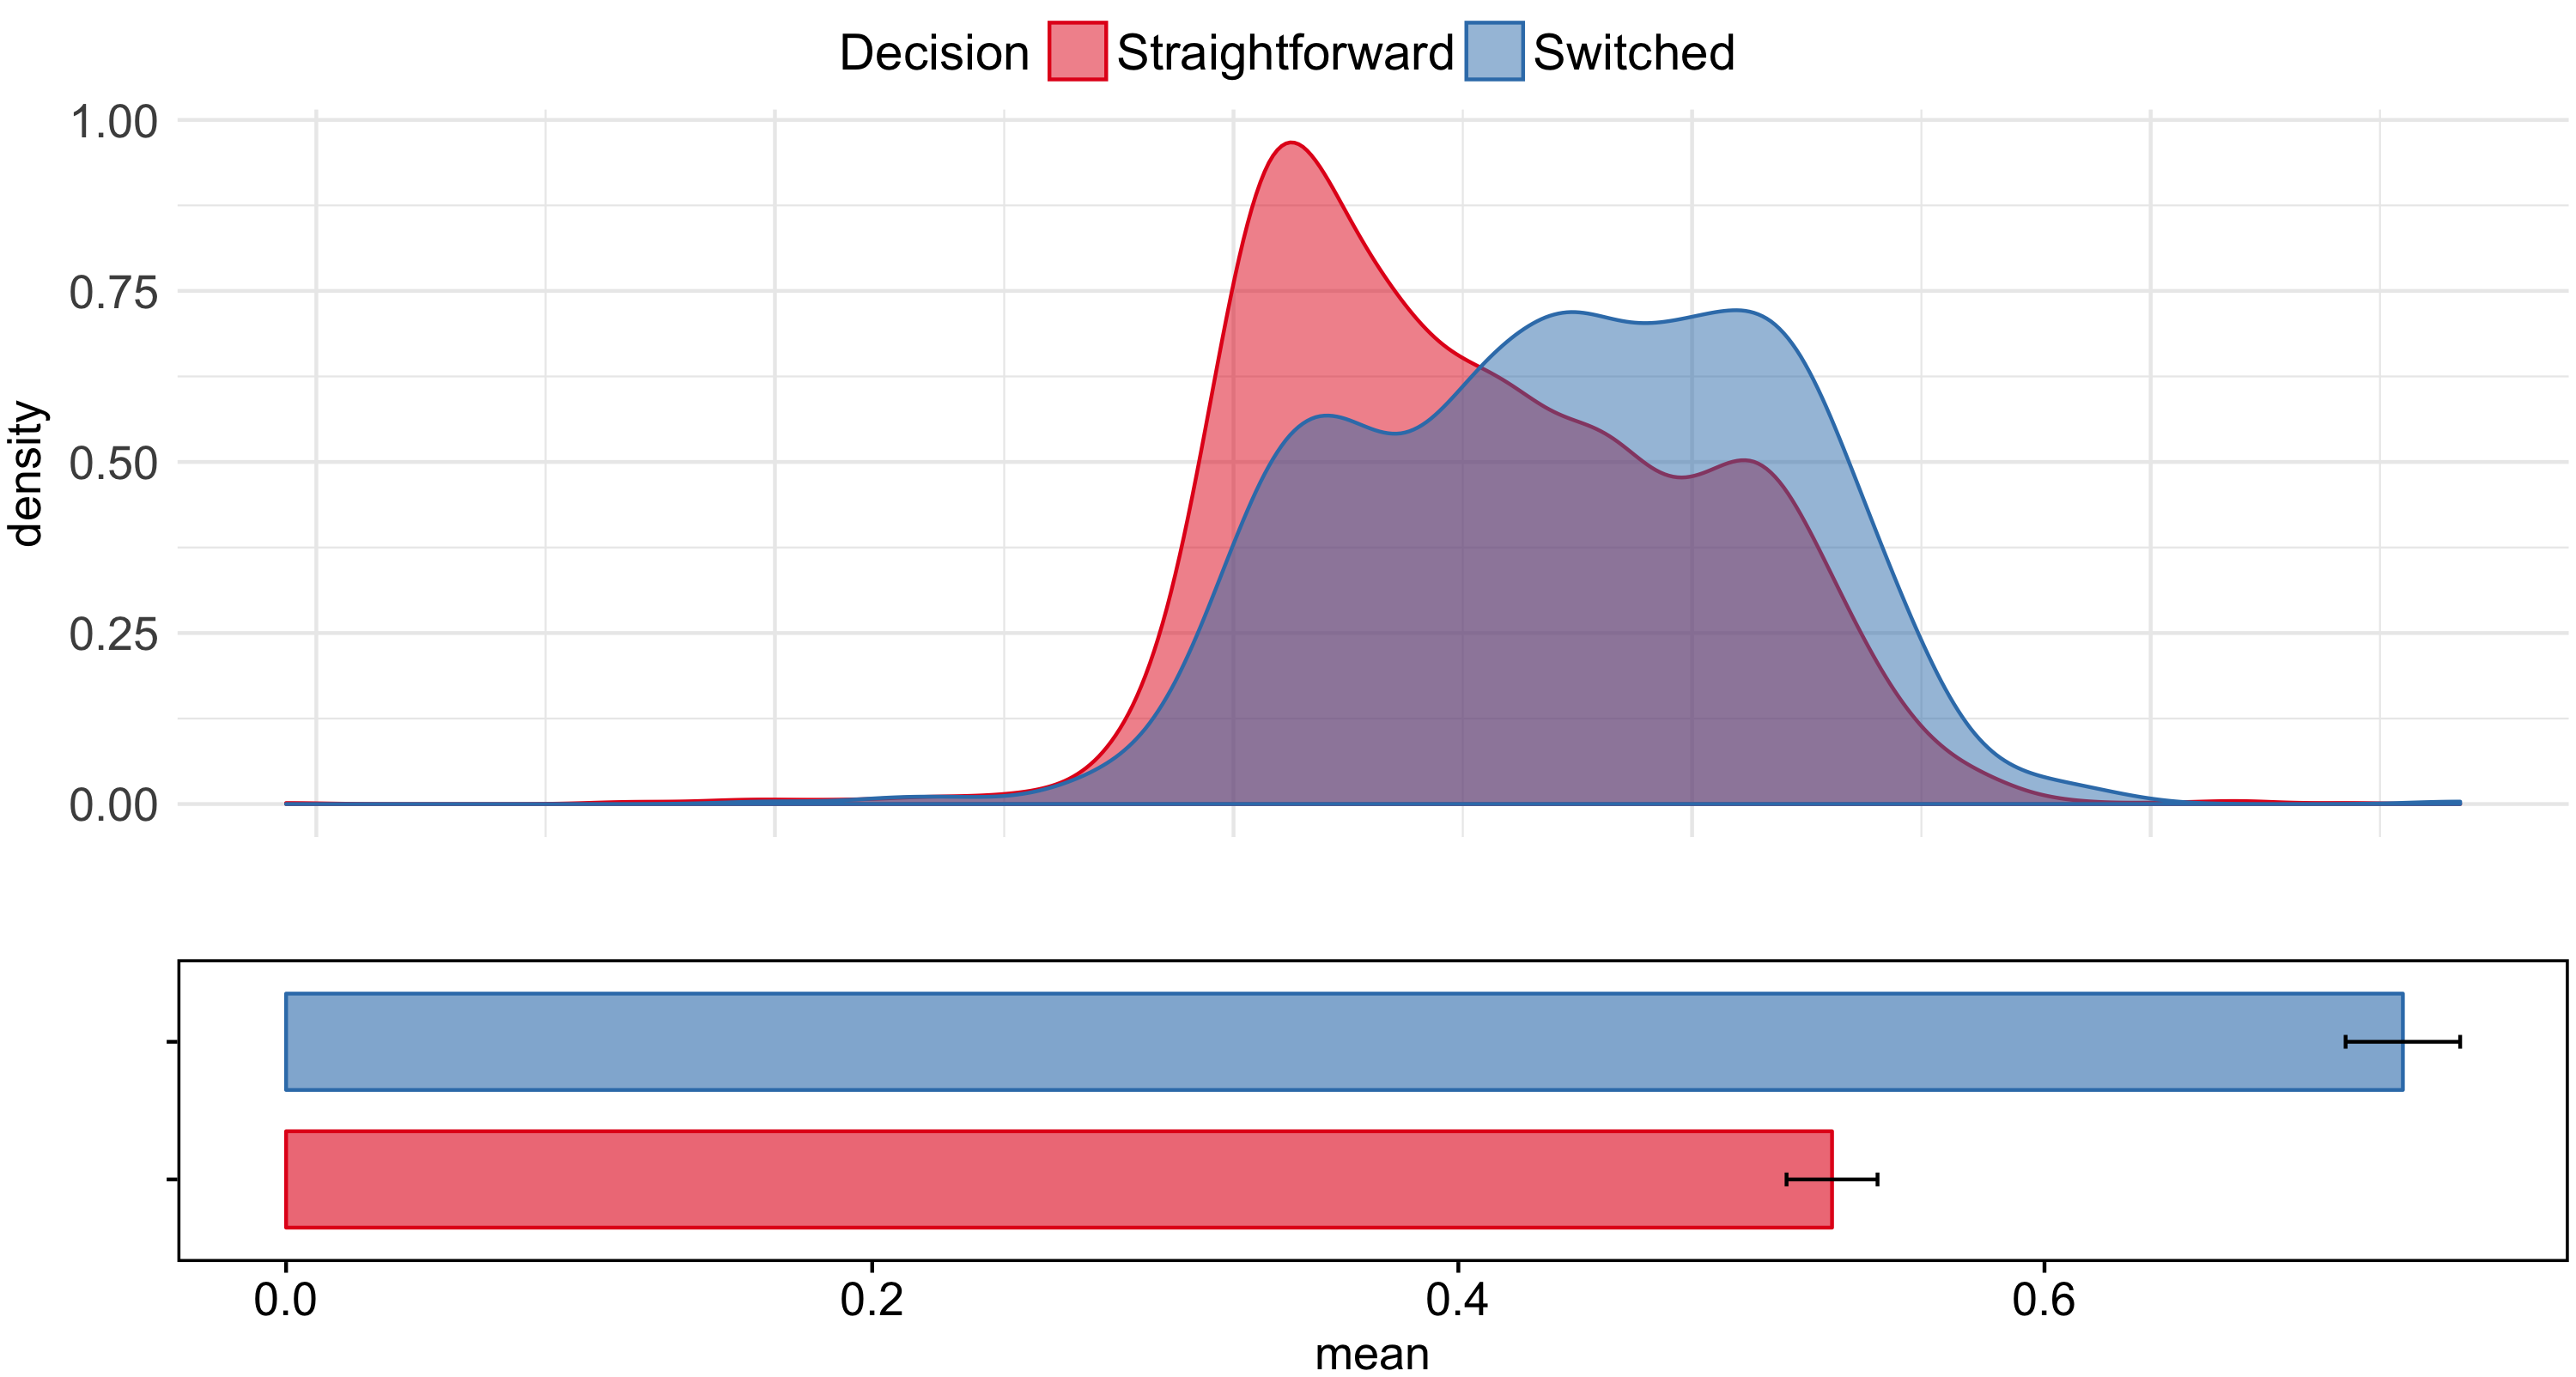
\includegraphics[width=\textwidth]{AUC_calibration.png}
\caption{Area Under the Trajectory}
\end{subfigure}
%
\begin{subfigure}[b]{0.4\textwidth}
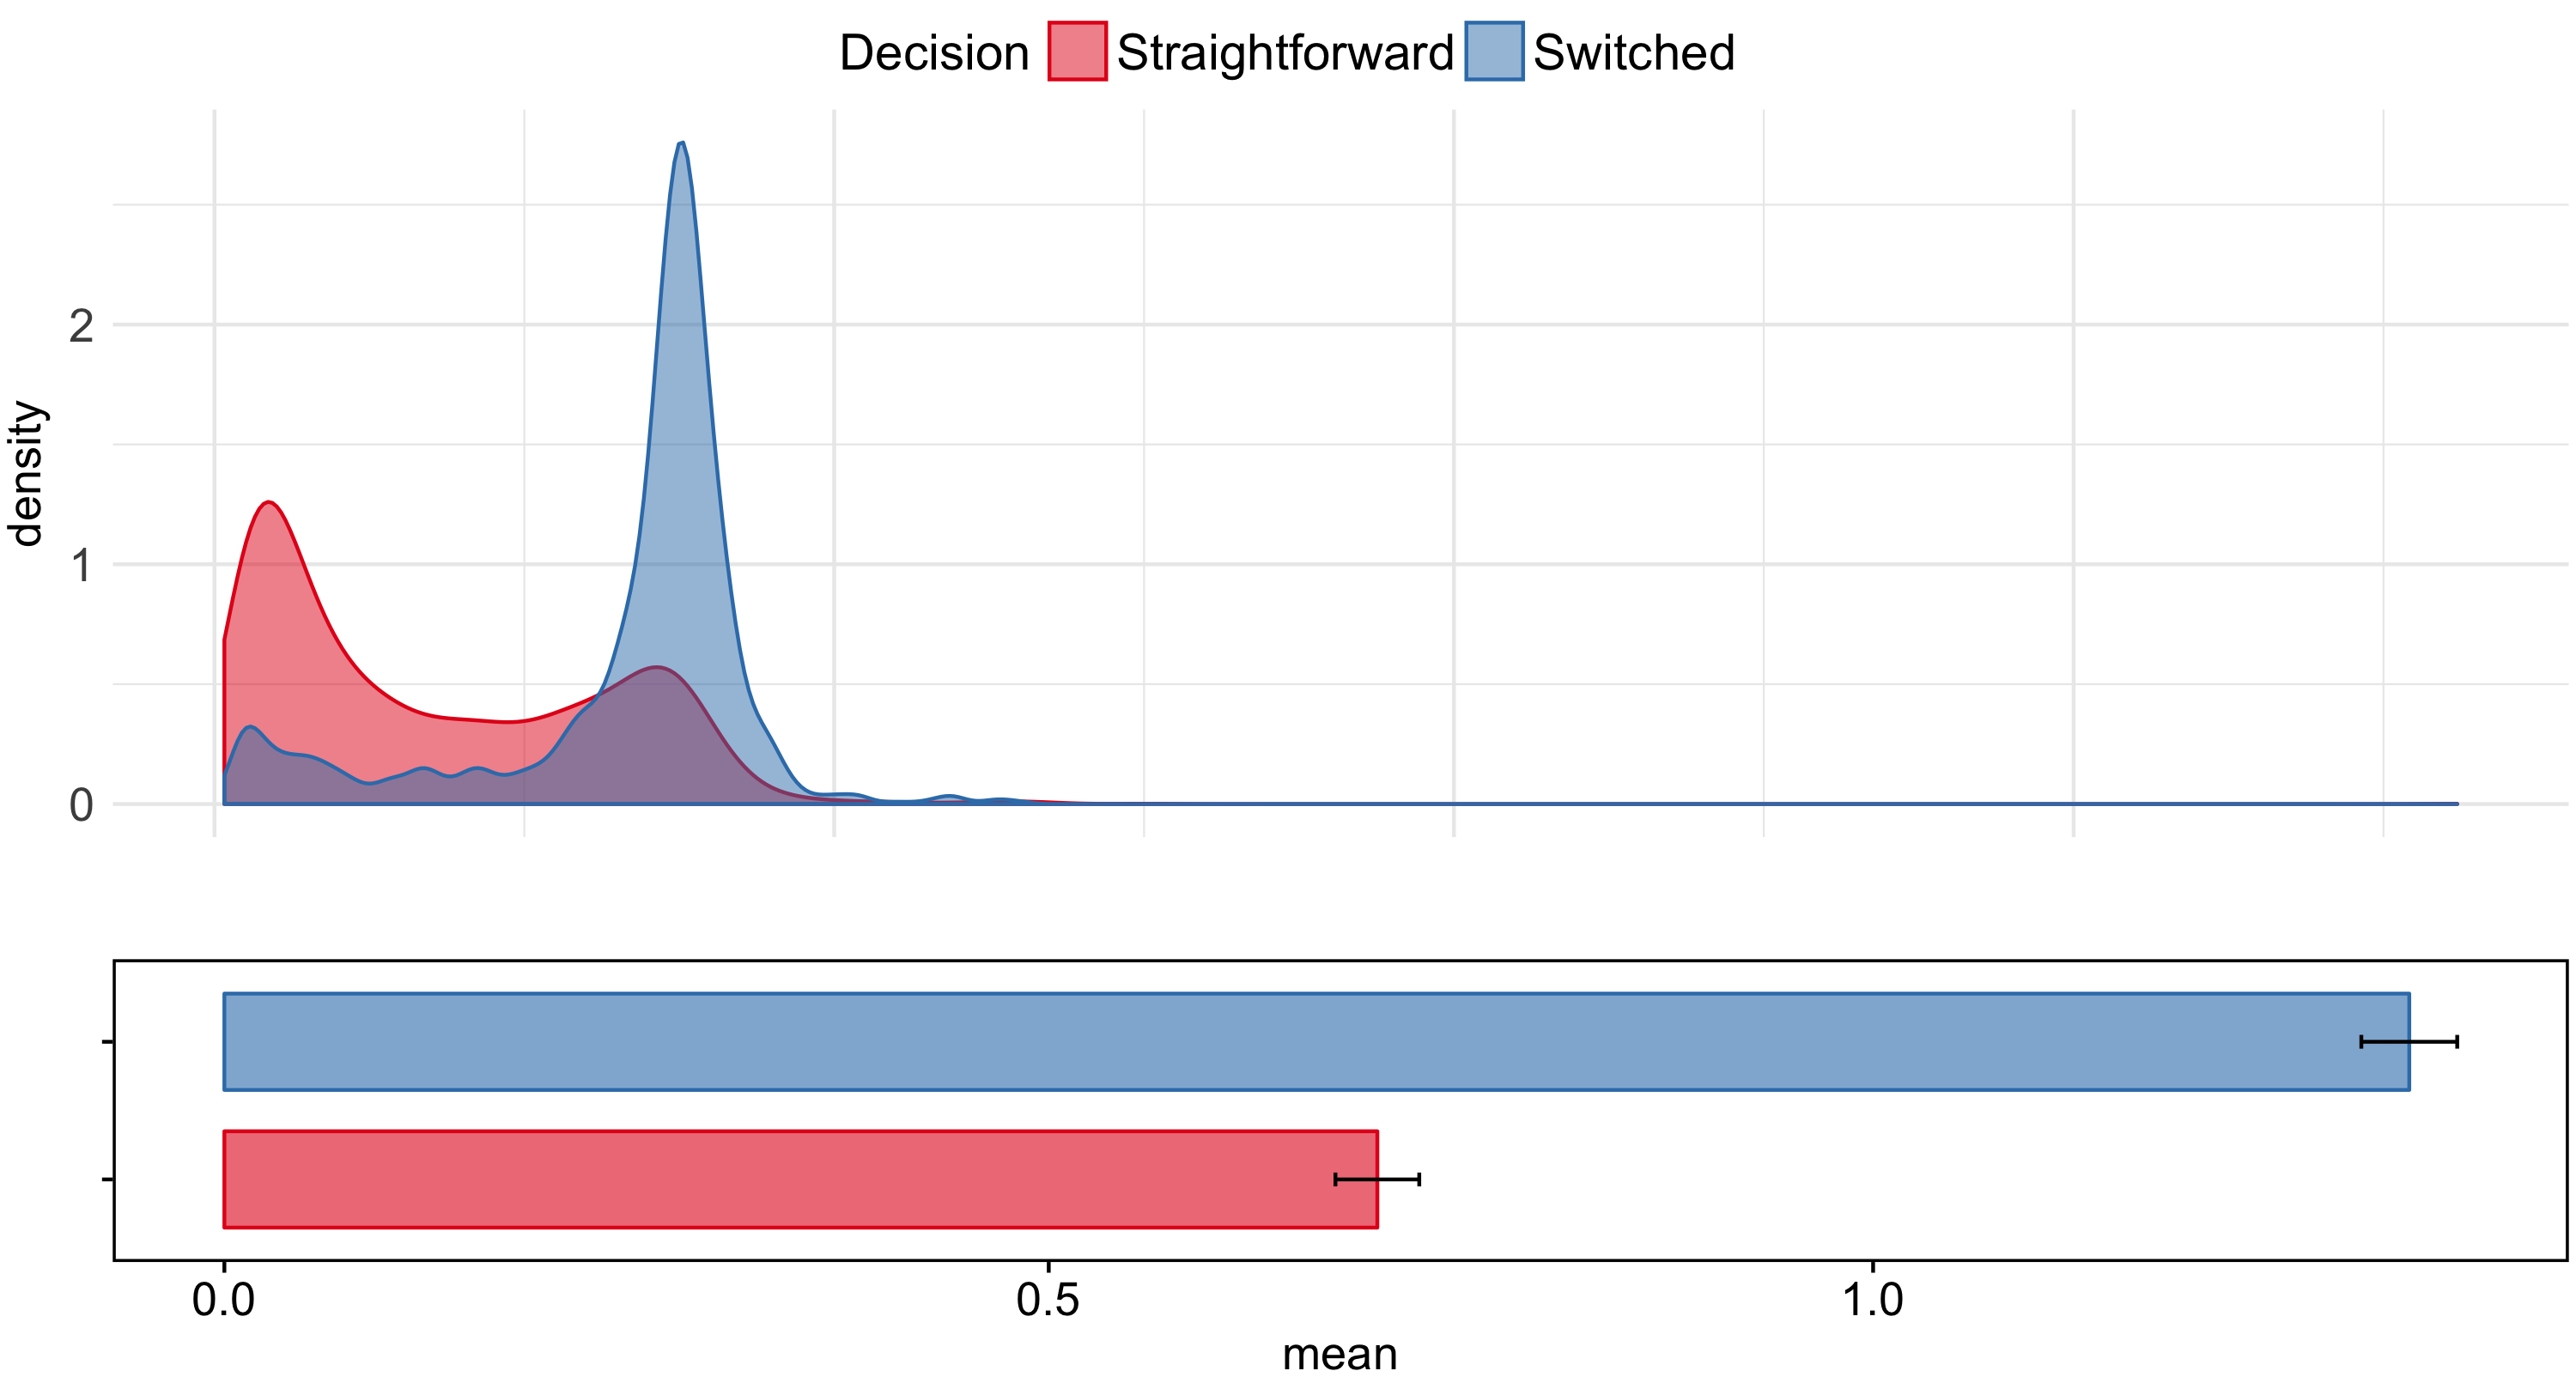
\includegraphics[width=\textwidth]{MD_calibration.png}
\caption{Maximal Deviation}
\end{subfigure}

%
\begin{subfigure}[b]{0.4\textwidth}
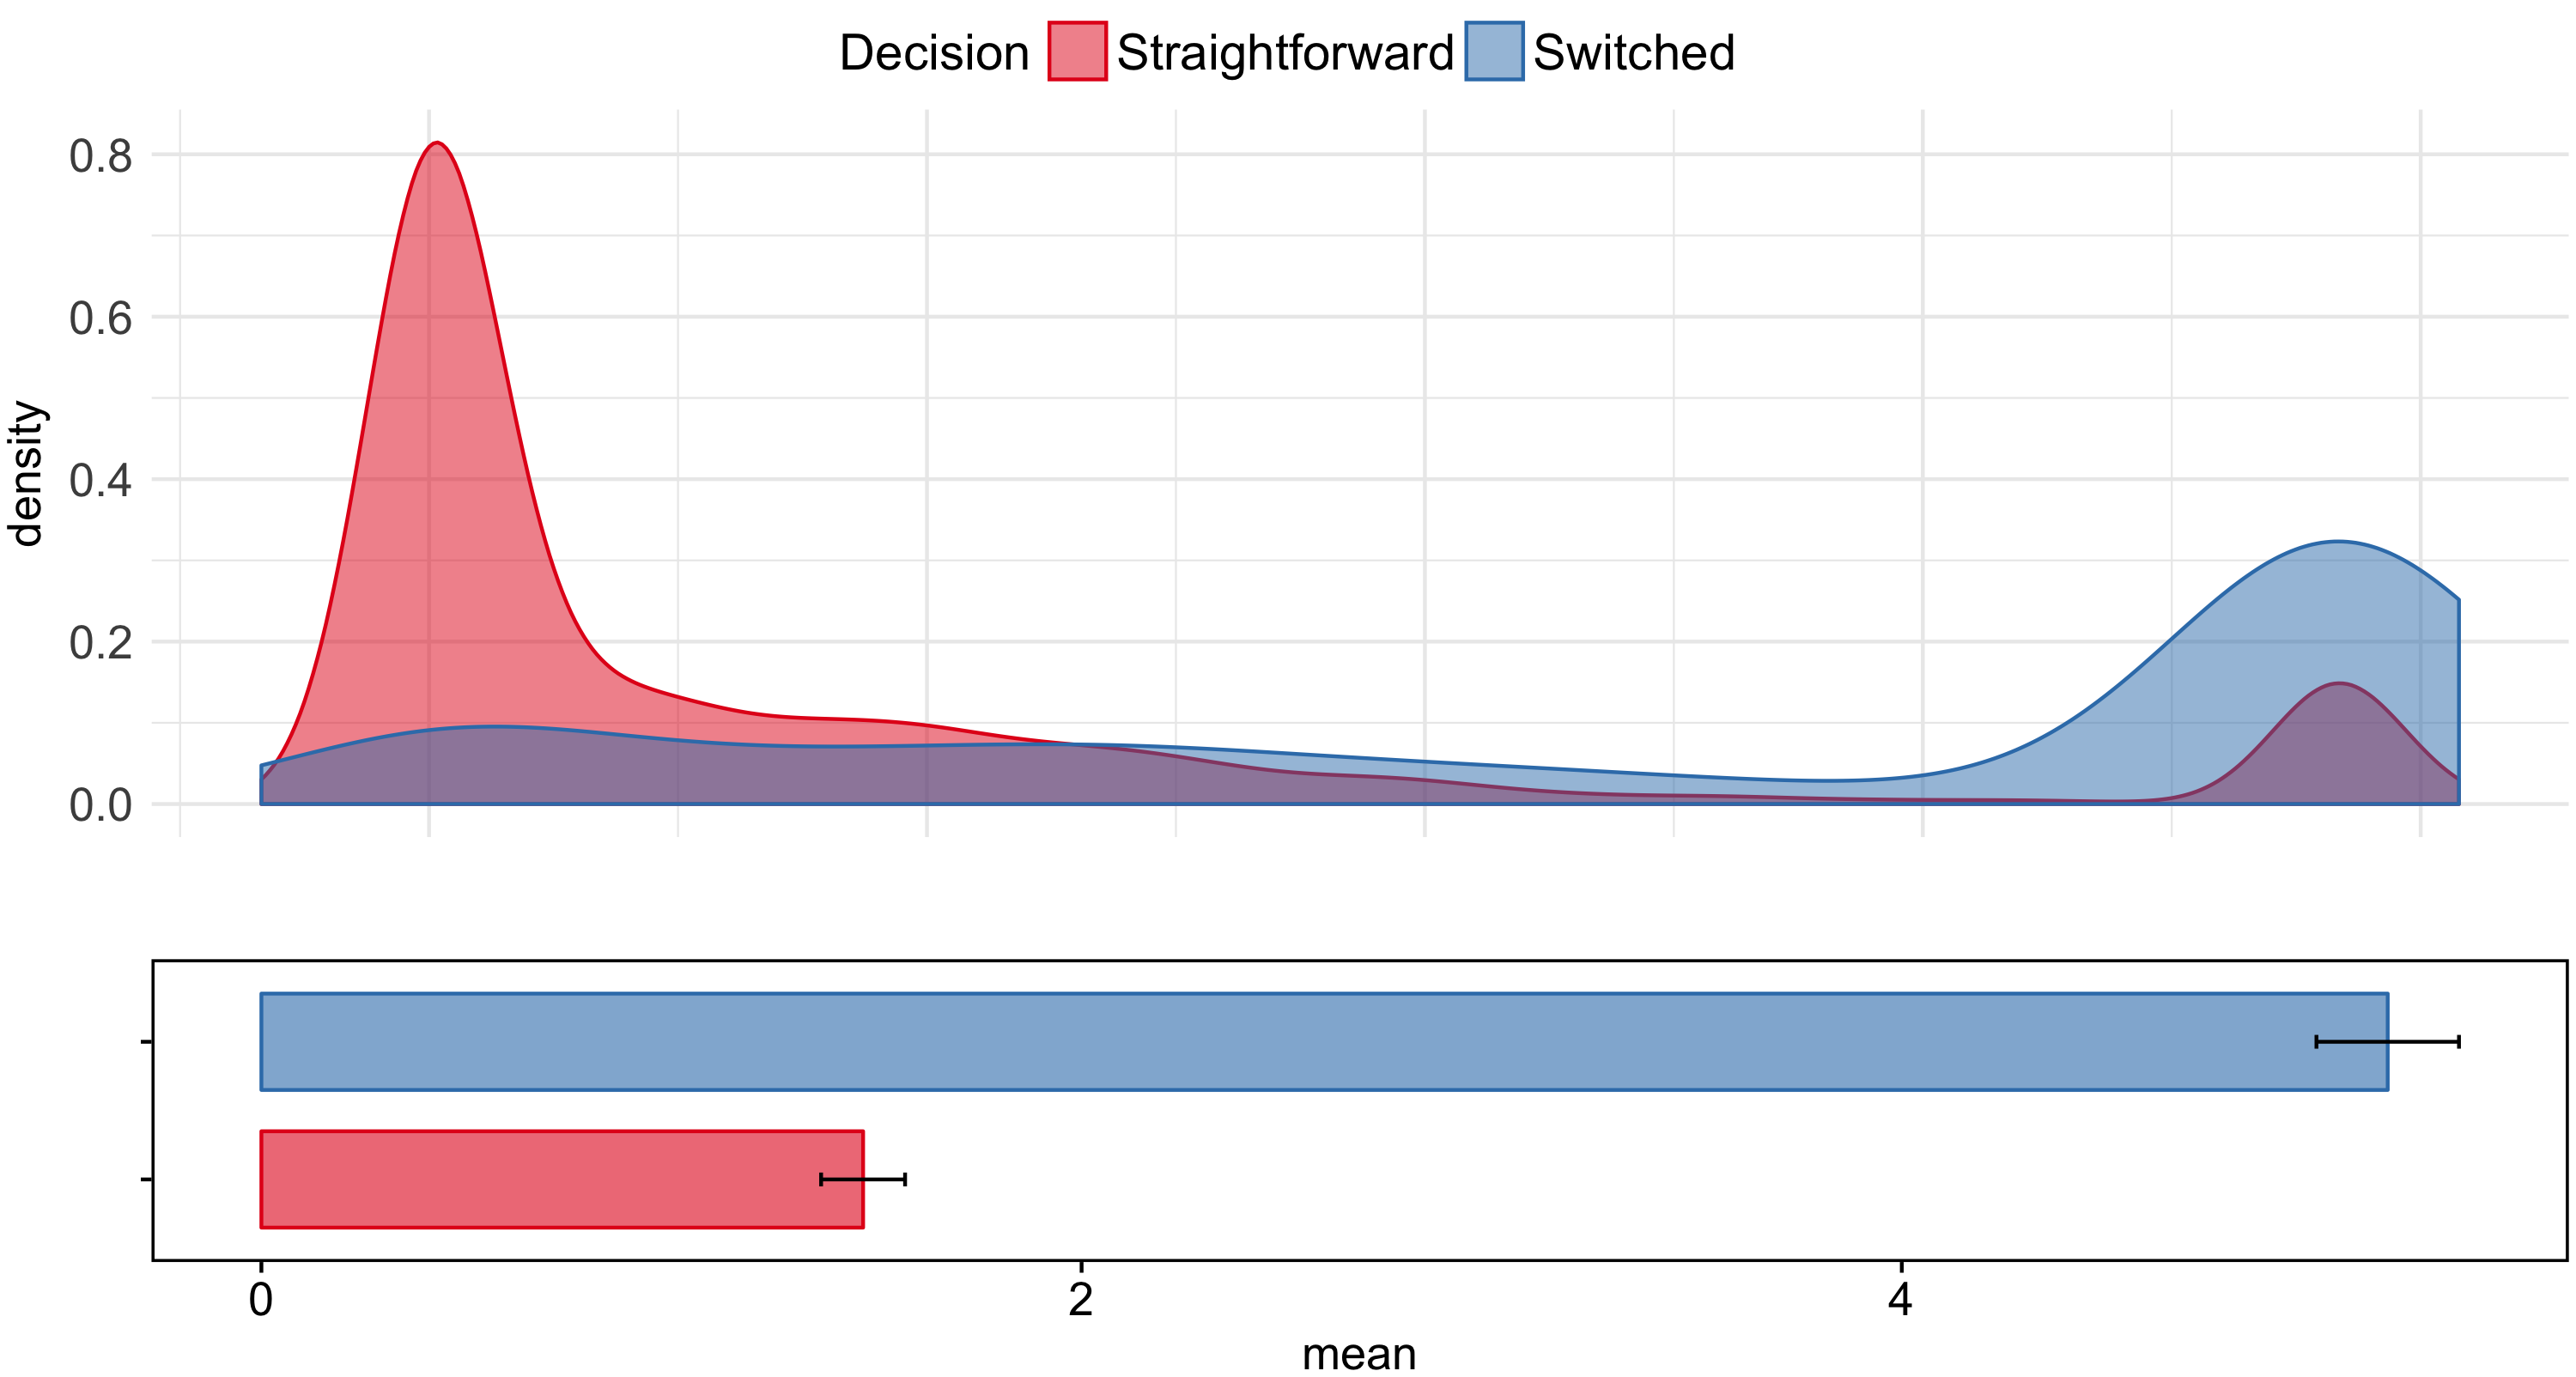
\includegraphics[width=\textwidth]{MaxRatio_calibration.png}
\caption{Maximal LogRatio}
\end{subfigure}
%
\begin{subfigure}[b]{0.4\textwidth}
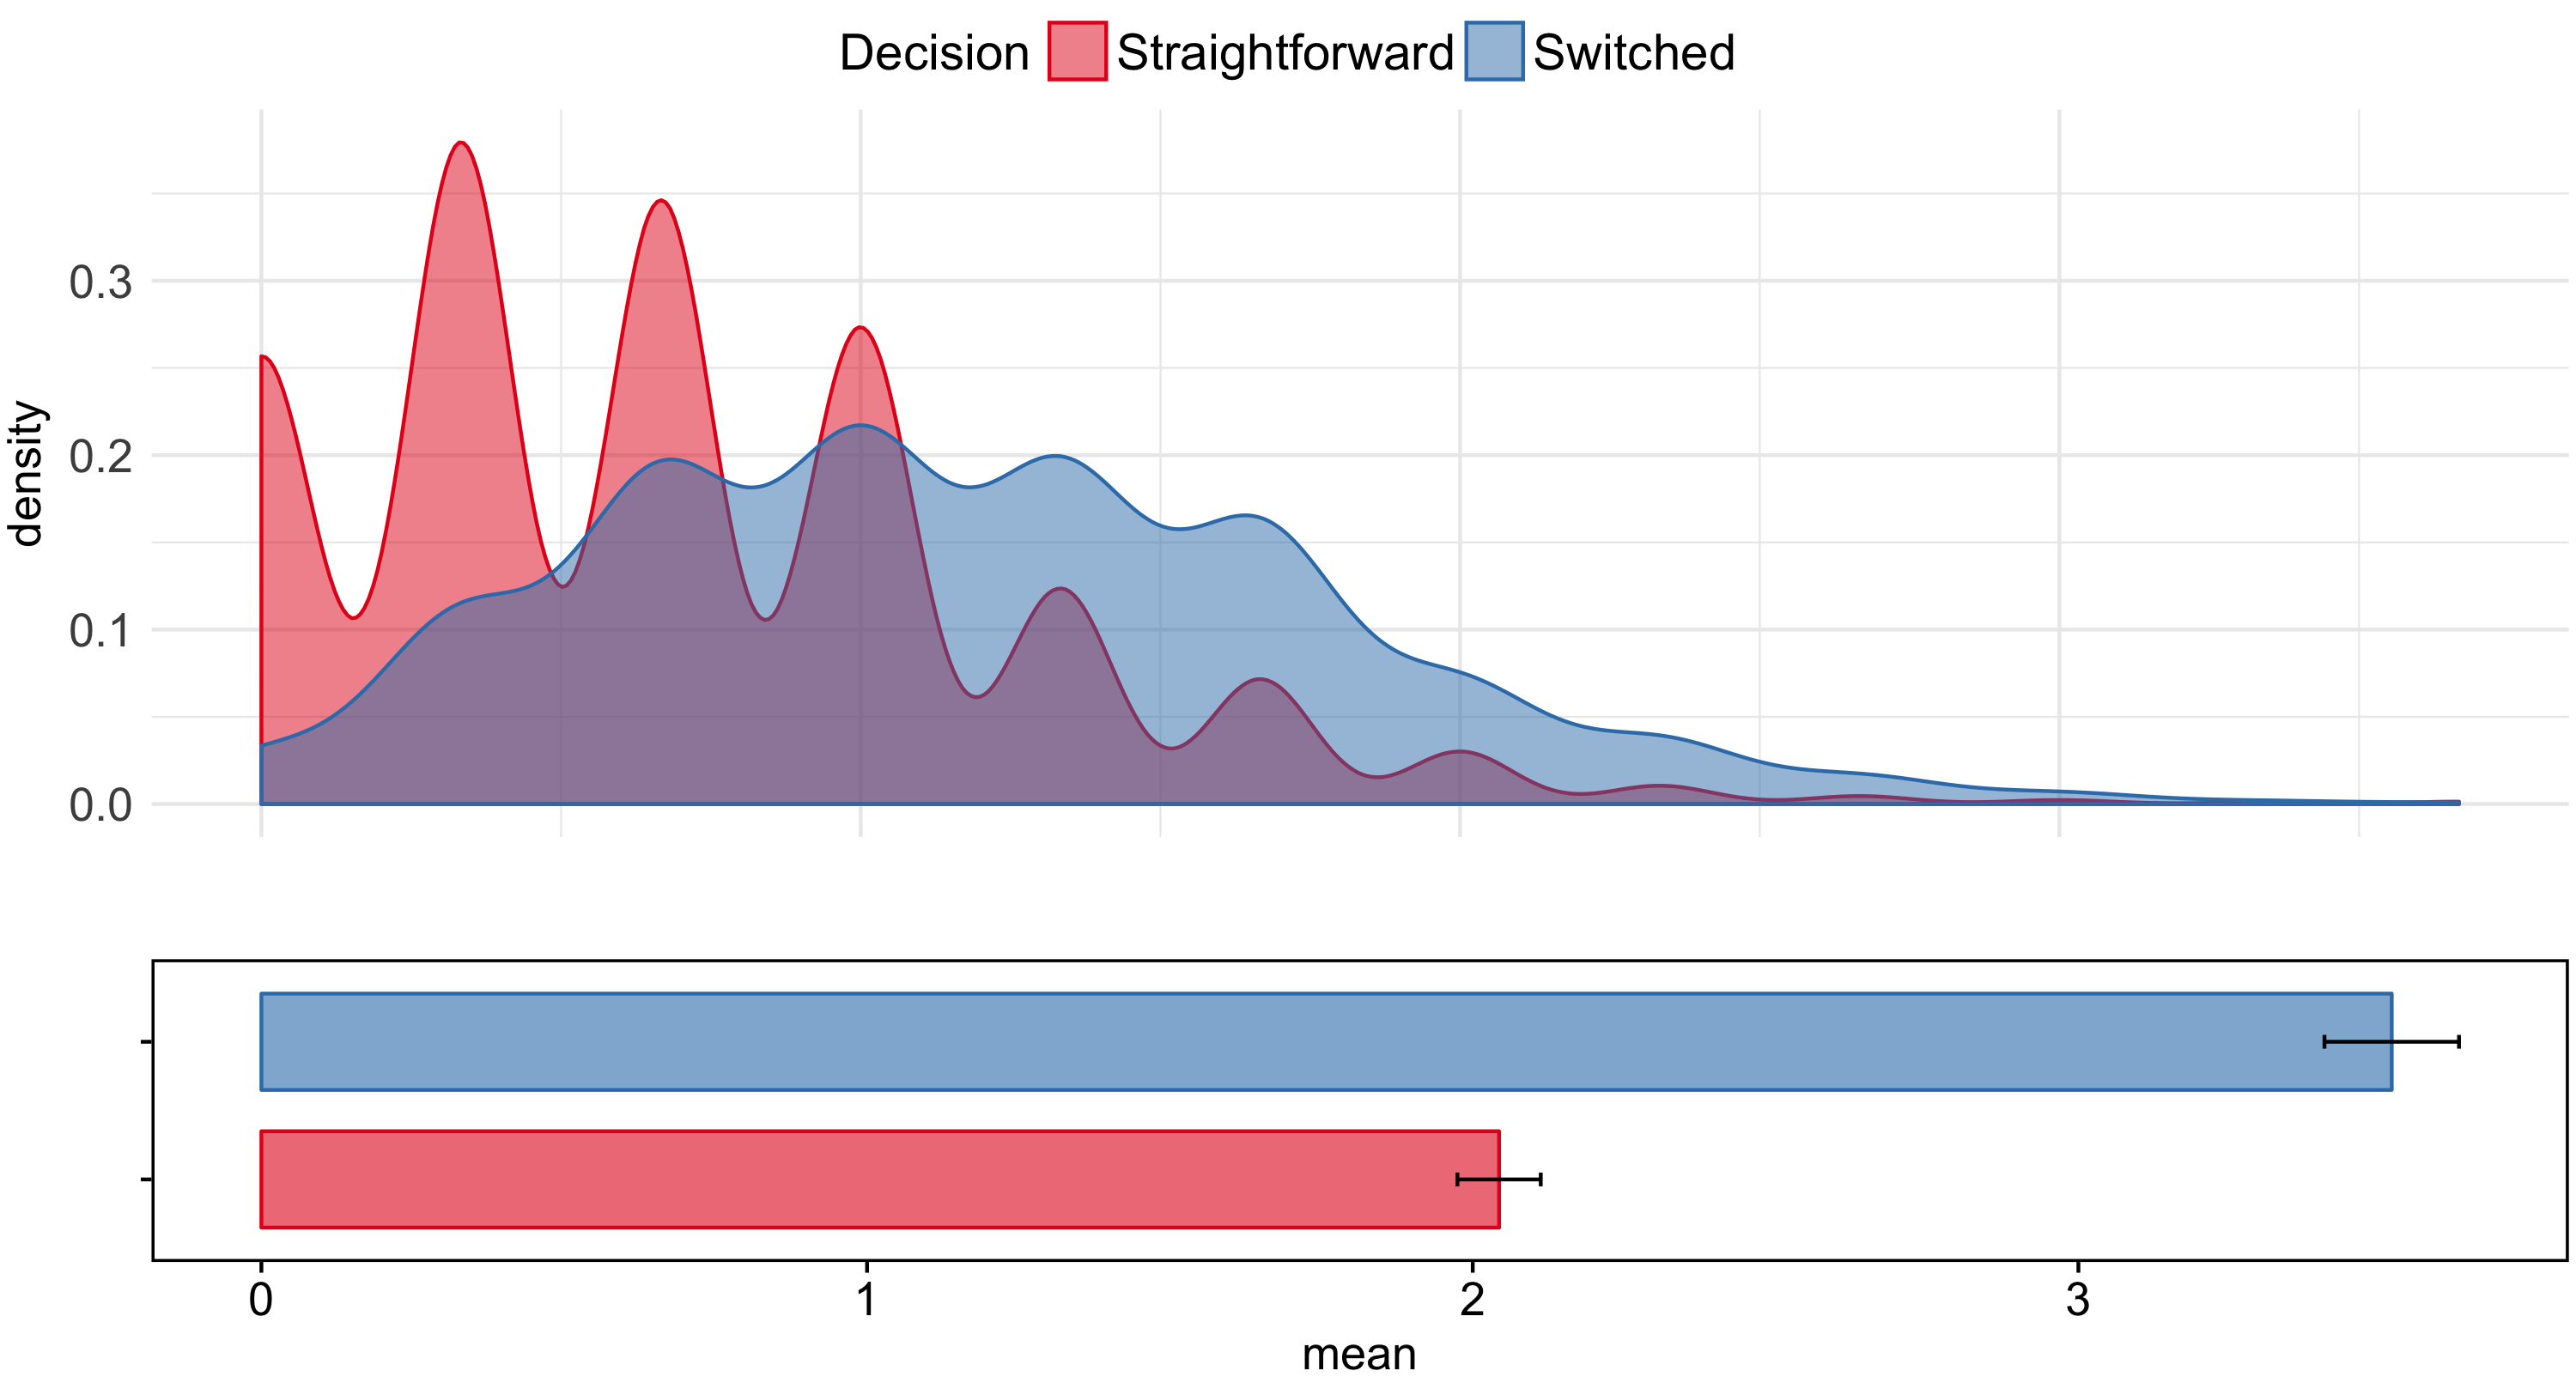
\includegraphics[width=\textwidth]{Xflips_calibration.png}
\caption{X-coordinates Flips}
\end{subfigure}

\begin{subfigure}[b]{0.4\textwidth}
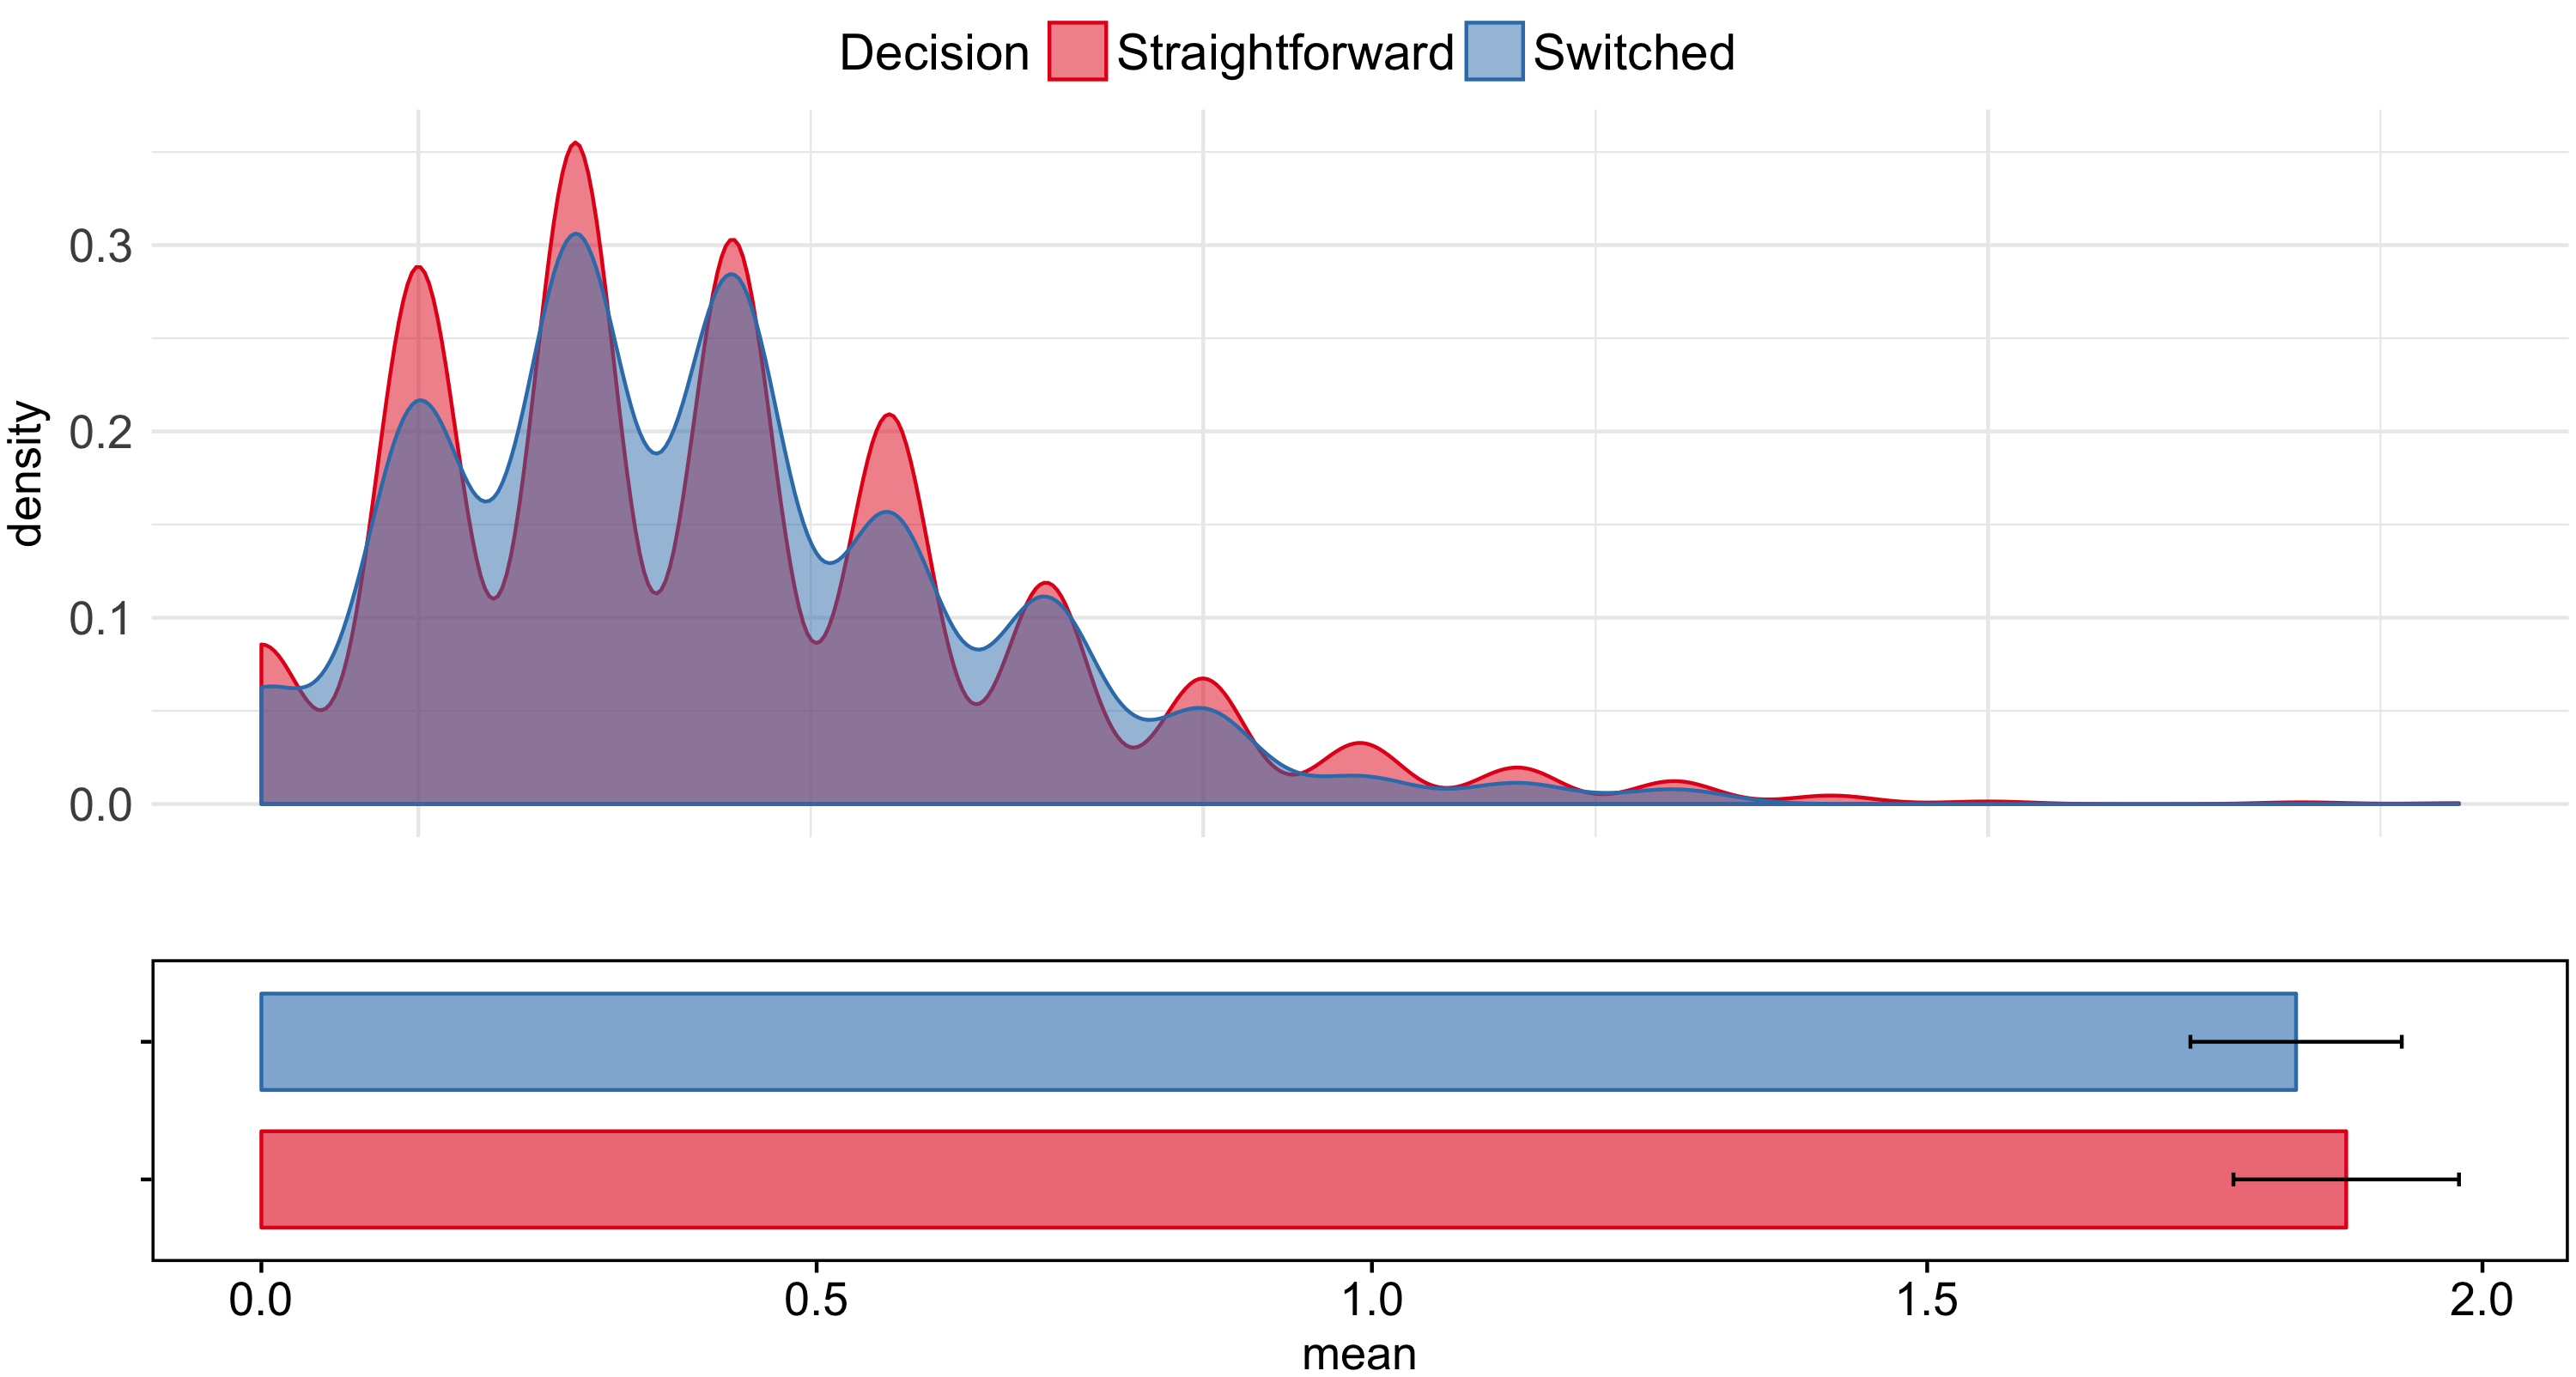
\includegraphics[width=\textwidth]{AC_calibration.png}
\caption{Acceleration Component}
\end{subfigure}

\caption{Different measures applied to Dale \& Duran replication.}
\label{fig:different.measures}

\end{figure}


\begin{figure}
\centering
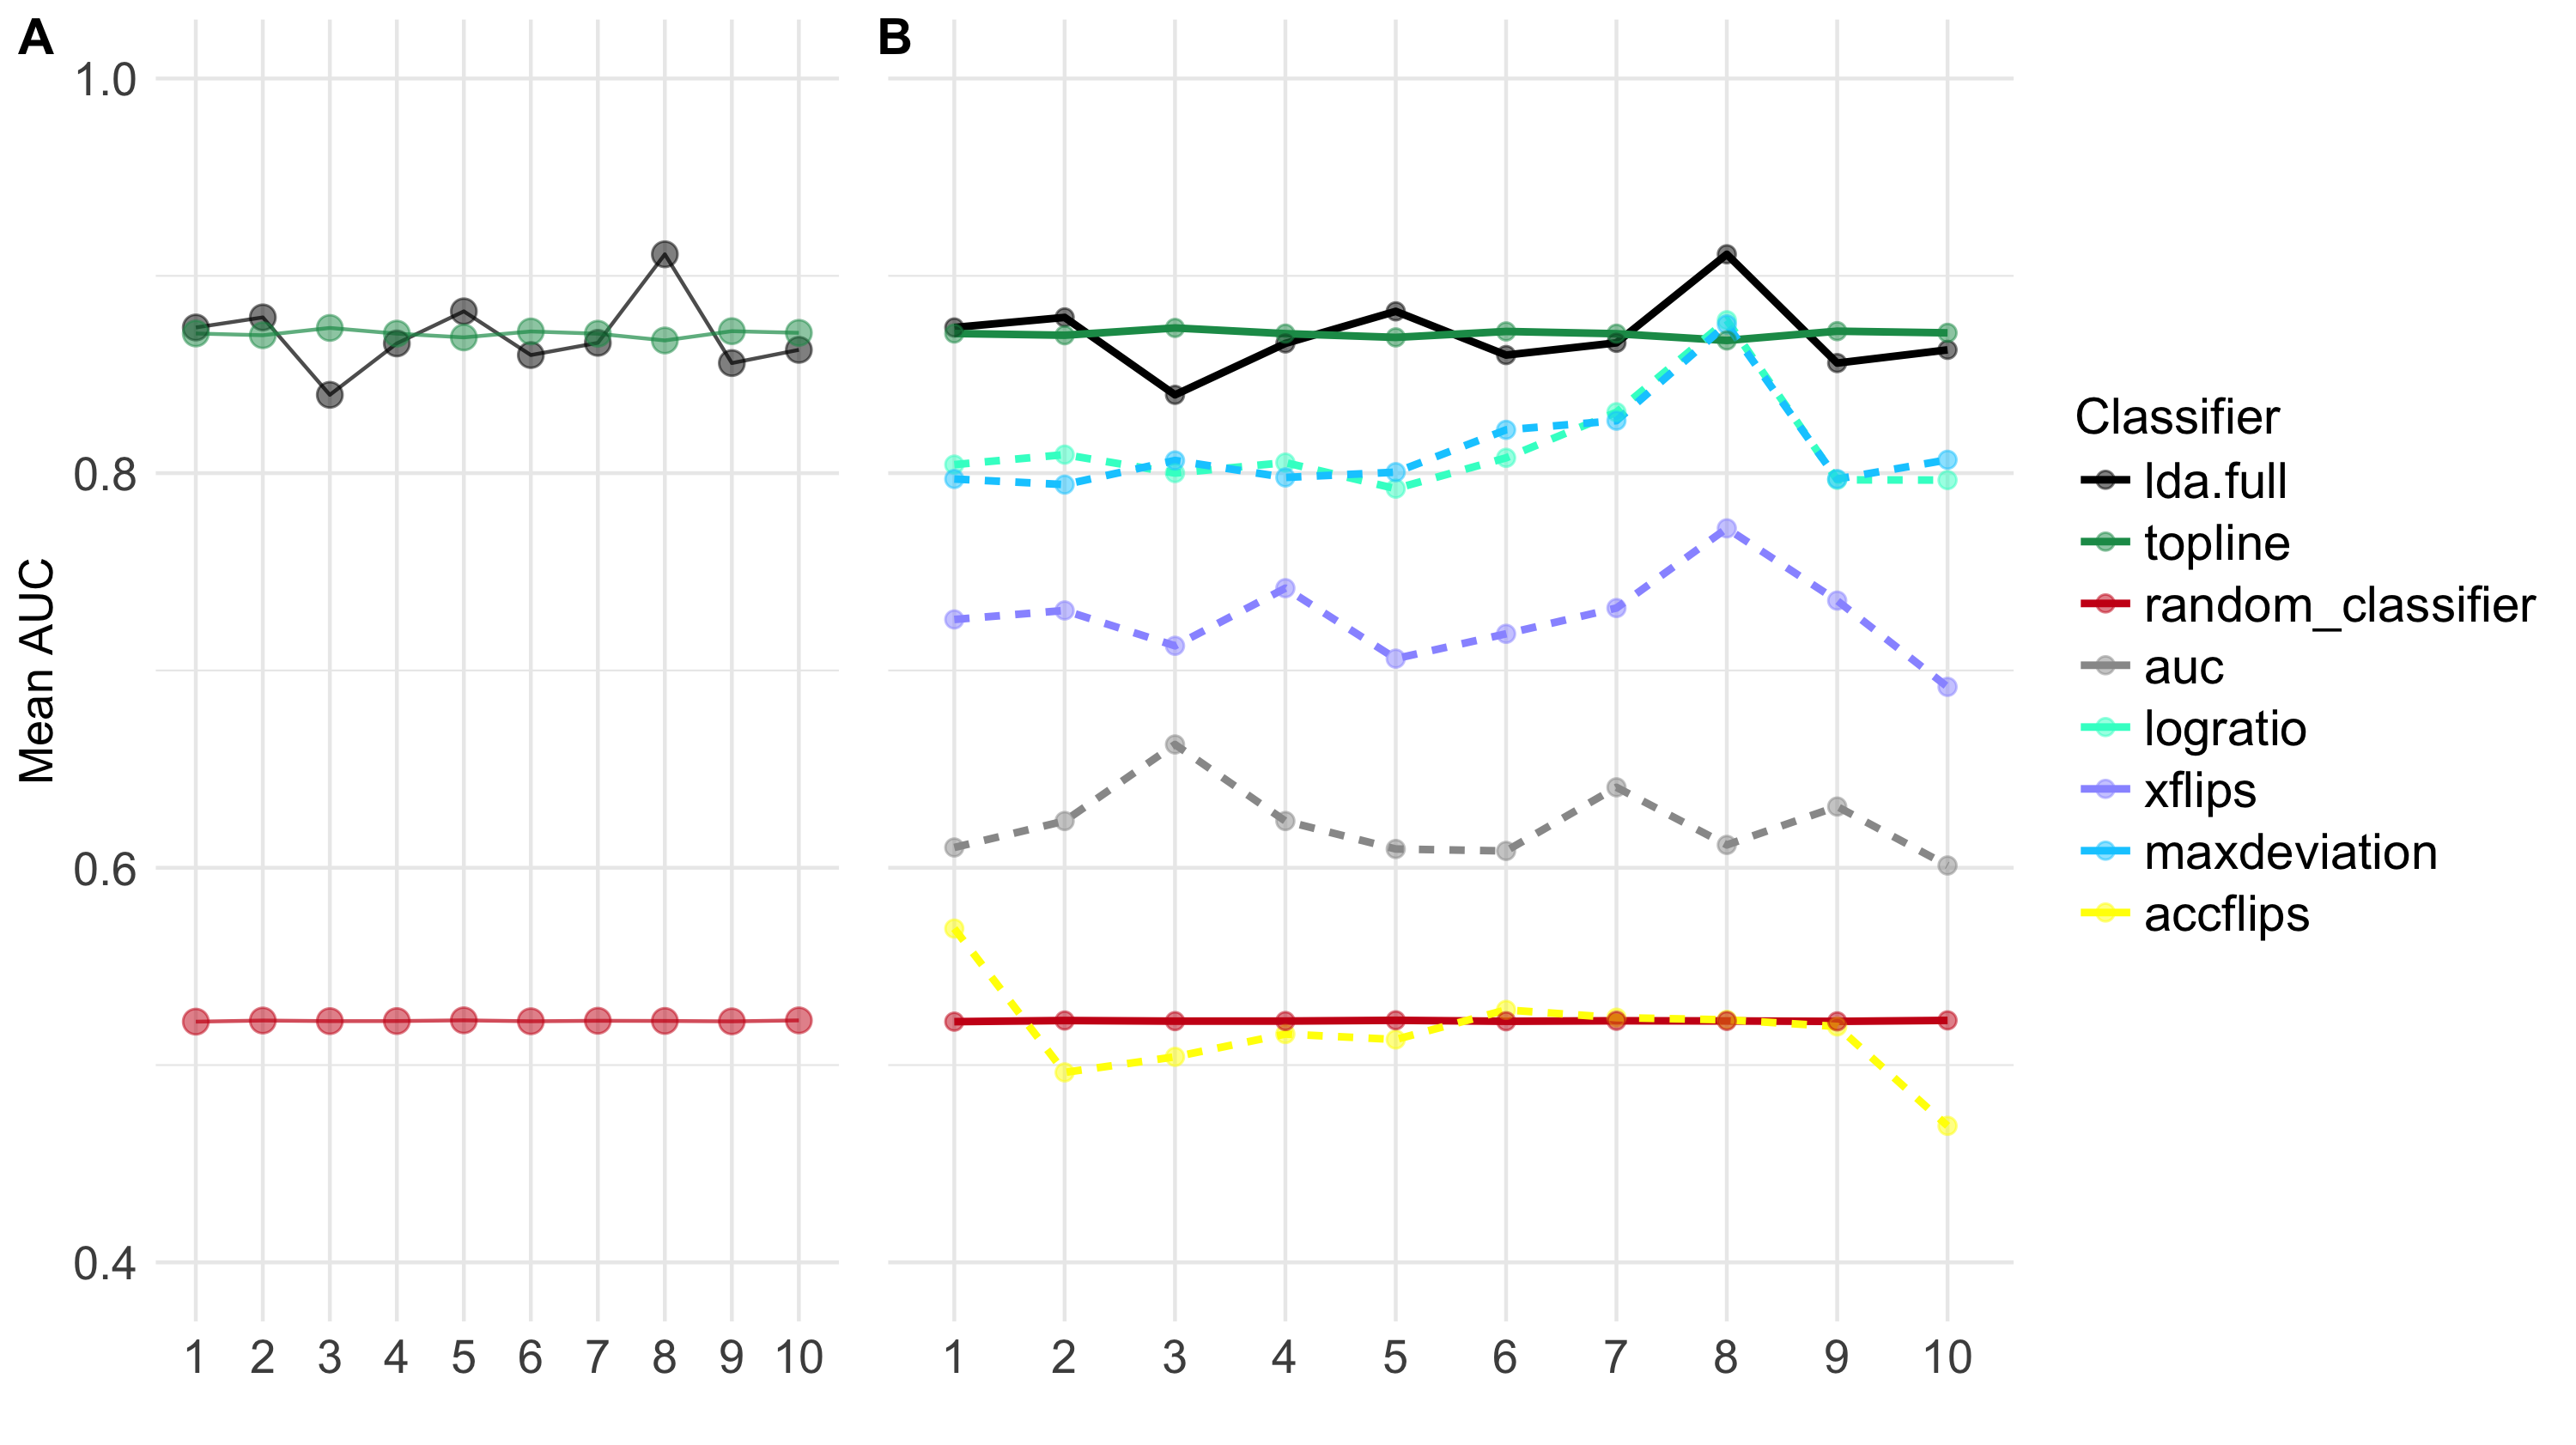
\includegraphics[width=\textwidth]{auc_calibration_3.png}
\caption{Mean AUC values}  \label{DIST:AUC2}
\end{figure}

\begin{table}[h]
\centering
{\small
\begin{tabular}{p{1.5cm}>{\columncolor[gray]{0.8}}p{1.5cm}cp{1.4cm}p{1.7cm}p{1.6cm}c}
& \centering \textsc{Original LDA}& \textsc{AUT} & \centering \textsc{MD} & \centering\textsc{Maximal LogRatio} & \centering\textsc{X-Coord. Flips} & \textsc{AC} \\

\hline
\centering \textbf{AUC (mean)} & \centering .87 & .62 &  \centering .81 &  \centering.81 & \centering.73 & .53 \\[0.5cm]
\hline 
\centering \textbf{Mean \\ Difference} & \centering--& .24 & \centering .06 &  \centering.06  & \centering .14 & .34  \\[0.5cm]
\hline
\centering \textbf{$p$ value} &\centering -- & \centering$<$.001&\centering $<$.001&\centering$<$.001&\centering$<$.001&$<$.001\\
\hline
\end{tabular}}
\caption{Cross-validation results for the LDA classifier. The performance of the LDA was compared to the one of five commonly used measures in mouse-tracking studies.}
\label{table:comparisons.permutation.2}
\end{table}
Overall, these comparisons reveal that the LDA is significantly better at classifying validation data than other commonly used measures. The difference with the classifier is in all the cases significant. Mean AUC values suggest that the MD and the Maximal LogRatio are better at distinguishing decision processes than other measures such as the Area, the number of X-coordinate flips, and the Acceleration Component. These two measures are the only ones calculated based on coordinates, and therefore give more importance to spatio-temporal information than the others. In other words, both the MD and the maximal log-ratio give different weight to positions depending the moment when they occurred, and therefore are more sensitive to the moment at which deviation occurred. This information seems to be essential for the classification, as observed in \Cref{section:LDA}. 

Finally, we previously observed that velocity and acceleration were not good predictors for the LDA classifier. Indeed, the performance of the Acceleration Component overlaps here with that of the baseline (i.e. random classification), suggesting that this type of information is not helpful.

\paragraph{}
We have shown that (i) a rough manipulation of decision making processes has a direct impact on mouse trajectories; (ii) a linear discriminant analysis (LDA) using absolute-temporal information is enough to accurately distinguish these quasi-decisions; and (iii) this LDA does a better classification than other traditional mouse-tracking measures. But, can our LDA can classify more complex decision processes, such as the ones involved in sentence verification tasks? 


\section{Extension to linguistic data}
\label{section:replication}
How well does our LDA, trained on “quasi-decisions”, classify new trajectories, which underly cognitive processes that might or not correspond to different decision patterns? To address this question, we test our classifier on data obtained from a replication of Dale and Duran's (\citeyear{Dale2011})  experiment.   
 
Dale and Duran (\citeyear{Dale2011}) found differences in the processing of true positive and negative sentences when people performed a simple truth-value judgment task. These results were interpreted as indicating that negation underlies an abrupt shift in cognitive dynamics (i.e. an unconscious change of decision). If this is indeed the case, we would expect mouse trajectories corresponding to the verification of negative sentences to pattern with \emph{switched} trajectories from the validation experiment. This pattern of results would provide additional support to the hypothesis that, at least in \emph{out-of-the-blue} contexts, processing negation does involve a `two-step' derivation, where the positive argument is initially derived and negated only as a second step\footnote{Note that the data used to train the classifier correspond to \emph{quasi}-decisions; namely, the training set is only an approximation of what should happen during an unconscious change of decision, such as the one expected for negation processing. As a result, we expect some aspects of the decision processes on sentence-verification data not to be captured by the LDA.}. 

%In this section, we aim to (1) replicate Dale \& Duran results when performing the same analyses as them, (2) to use our classifier (trained with validation data) to test these processing differences, and (3) compare the performance of our classifier with the one of other measures. 


\subsection{Experiment}
Participants were asked to perform a truth-judgment task, where they had to decide whether a sentence (e.g. \textit{Cars have wheels}) is true or false according to common knowledge. Each of the sentences could be either a true or a false statement in its negated or non-negated form. 
Unlike Dale and Duran's experiment, the complete statement was presented in the middle of the screen after participants pressed ``start" (i.e. no self-paced reading). The ``true" and ``false"  boxes appear at the top-left or top-right corners of the screen, in the same way as in our validation experiment.  
An illustration of the sentences used as examples is provided in \Cref{table:exampleDD}. 

\paragraph{Participants}
53 English native speakers were tested using Amazon Mechanical Turk. They were rewarded for their participation. The experiment lasted approximately 10 minutes. 

\paragraph{Design}
The experimental design consisted of two fully crossed factors: \textsc{Truth value} (true, false) and \textsc{Sentence polarity} (negative, positive). We had a total of 4 conditions, and each participant saw 4 instances of each condition (16 sentences). 


\begin{figure}
\centering
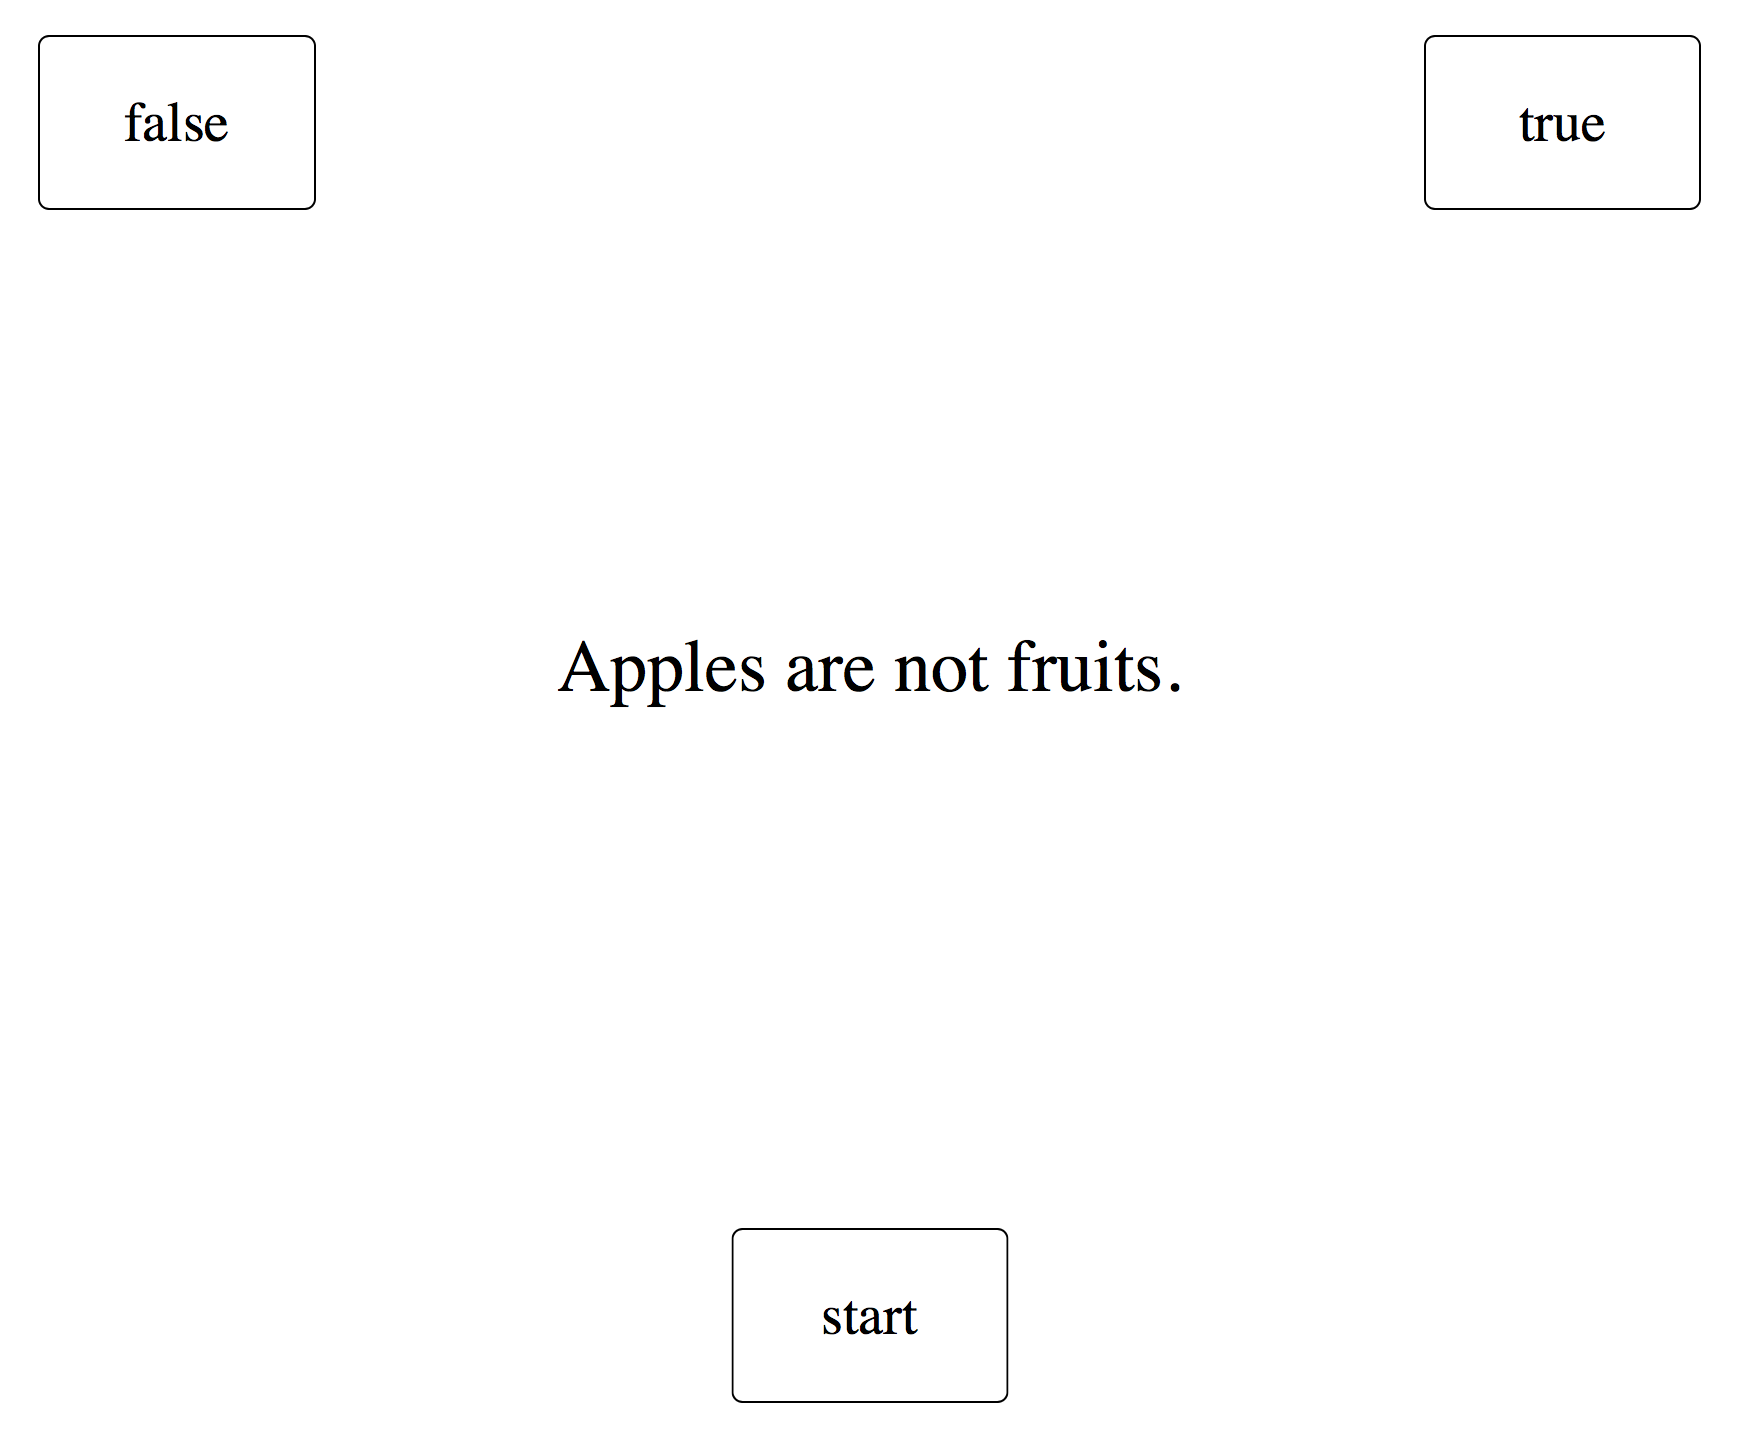
\includegraphics[width=0.7\textwidth]{trial_example2.png}
\caption{Illustration of a Trial in Dale \& Duran's Replication}
\end{figure}



\begin{table}[h]
\centering
\begin{tabular}{ccc}
Truth value & Polarity & Example \\
\hline
\multirow{2}{*}{True} & Positive & Cars have wheels.\\ 
 & Negative & Cars have no wings.\\ 
\hline
\multirow{2}{*}{False} & Positive & Cars have wings.\\ 
 & Negative & Cars have no wheels.\\
\end{tabular}
\caption{Design} \label{table:exampleDD}
\end{table}


\paragraph{Interface and data treatment}
The interface and data treatment were the same as the ones used for the calibration experiment. Mouse trajectories' time course was normalised into 101 time steps.

\subsection{Results and discussion}
\paragraph{Replicating Dale and Duran (2011)}
All participants responded correctly more than 75\% of the time. No participant was discarded based on accuracy.  Only accurate trials were taken into account for the analyses. \Cref{fig:mean.trajectory-negation} illustrates mean trajectories for the four possible trial conditions.
\begin{figure}
\centering
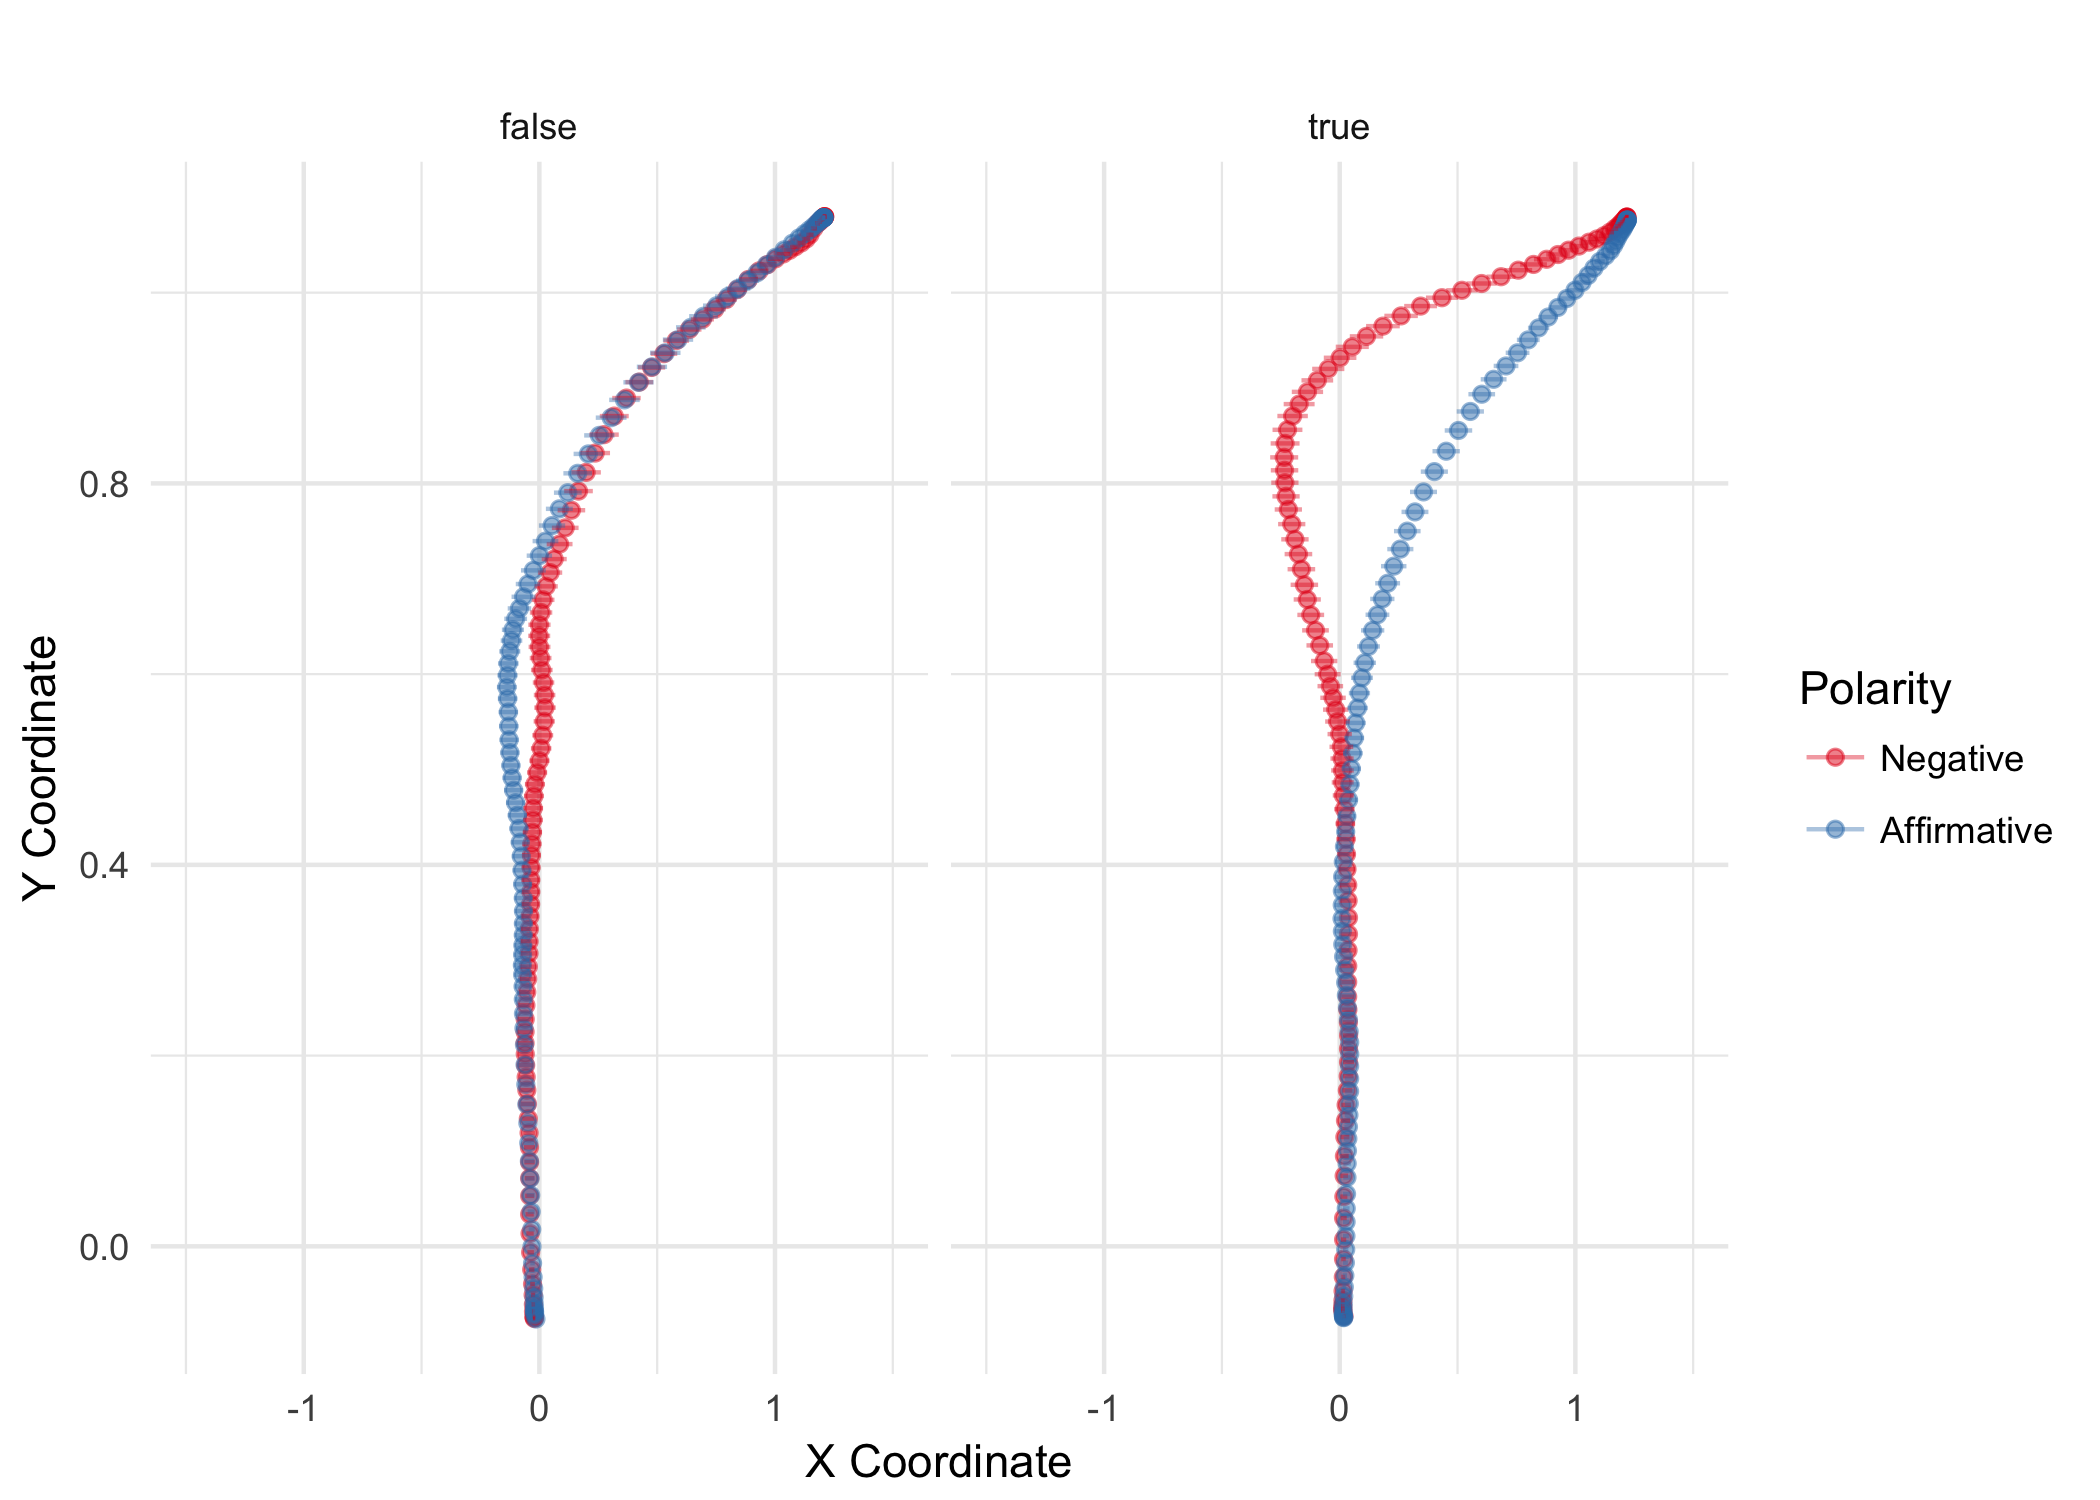
\includegraphics[width=0.7\textwidth]{negation-data-mean-trajectory.png}
\caption{Mean trajectories for accurate trials} \label{fig:mean.trajectory-negation}
\end{figure}

To assess whether we replicate Dale and Duran's results, we calculated the $x$-coordinate flips (see \Cref{section:other-mt}) and analysed them with a linear mixed-effects model \citep{baayen2008mixed}, taking \textsc{Truth}, \textsc{Polarity} and their interaction as predictors. We included random intercepts per subject and a random slope with the interaction of both factors. $P$-values were obtained by comparing the omnibus model to a reduced version of itself, where the relevant factor was removed. This pipeline mirrors the model performed by Dale and Duran. 

Unlike Dale and Duran, we did not perform statistical analyses based on the acceleration component (i.e. acceleration flips). 
In our validation experiment, this quantitative measure was unable to distinguish mouse trajectories underlying different ``quasi-decisions''.
The origin of this inadequacy is hard to determinate: it could be a property of the kind of decisions were are manipulating, or just a consequence of noisy data. We reasoned that if the different decision processes involved in a rather simple task were not captured by the acceleration component, this measure might also be unable to classify more complex processes, such as the ones at play in a sentence verification task. 

The model of x-coordinate flips revealed a main effect of \textsc{Polarity}, such that negation significantly increases flips in the $x$-coordinate by 0.76 ($\chi^{2}=10.11; p=.0014$), and a significant interaction \textsc{Truth} $\times$ \textsc{Polarity} ($\chi^{2}=22.7; p<.001$), such that the difference between negative and positive sentences is bigger for the true than for the false statements. There was no significant effect of \textsc{Truth} ($\chi^{2}<1; p=.5$). 
\Cref{table:negationresults} summarises the pattern of means and estimates for both ours and Dale and Duran's results. 

\begin{table}[h]
\begin{center}
\begin{tabular}{ccc}
Condition & $x$-flips &  $x$-flips in D\&D \\
\hline
T/no negation & 2.22 & 1.13 \\
T/negation & 3.67 & 1.71 \\
F/no negation & 2.82 & 1.24 \\
F/negation & 2.9 & 1.34 \\
Estimate Polarity & .76 & 0.35 \\
Estimate Truth & .07 & 0.13 \\
Estimate Truth$\times$Polarity & 1.35 & 0.47\\
\end{tabular}
\caption{Mean and effect estimates}
\label{table:negationresults}
\end{center}
\end{table}%

These results seem to replicate Dale and Duran's findings: Verifying true negated sentences produces less straightforward trajectories than true positive sentences (i.e. negation gives rise to more `curvy'/\addMM{rough?} trajectories). The values obtained in the two experiments, however, are slightly different; namely, our results present higher range of values (see \Cref{table:negationresults}). 
Note that, in our experiments, the mouse-position was not sampled at a fixed rate (see Interfase and data treatment), creating additional noise which could be responsible for the range difference\nbMM{maybe foonote?}. 

Our findings therefore pattern with a broader set of psycholinguistic studies, which, using different techniques, have revealed that the positive argument plays a role in negation processing: verifying negative sentences might involve computing the positive content at an early processing stage \citep{Tian2016}. 

\paragraph{Classifier performance}
Two different LDA classifiers, trained with data from the validation experiment, were applied to the new experimental data. The first classifier was our original LDA, which had as predictors $x,y$ coordinates as well as distance-based velocity and acceleration. The second LDA had only $x,y$ coordinates as predictors. Validation results (see \Cref{section:LDA}) suggest that the simpler model, which only relies on absolute information, might be sufficient to classify the two basic kinds of decision-making processes. That is to say, the simple model might fit the data as well as a more complex model, and be interpreted more straightforwardly. 

The relevant difference in processing between positive and negative sentences is expected to arise specifically for \emph{true} statements -- there is an interaction with truth values. Consequently, we analyse the performance of both classifiers when applied to true trials. \Cref{fig:lda_negation} illustrates the distribution and means of the resulting \textit{LDA measure}. 


\begin{figure}
\centering
\begin{subfigure}[b]{0.45\textwidth}
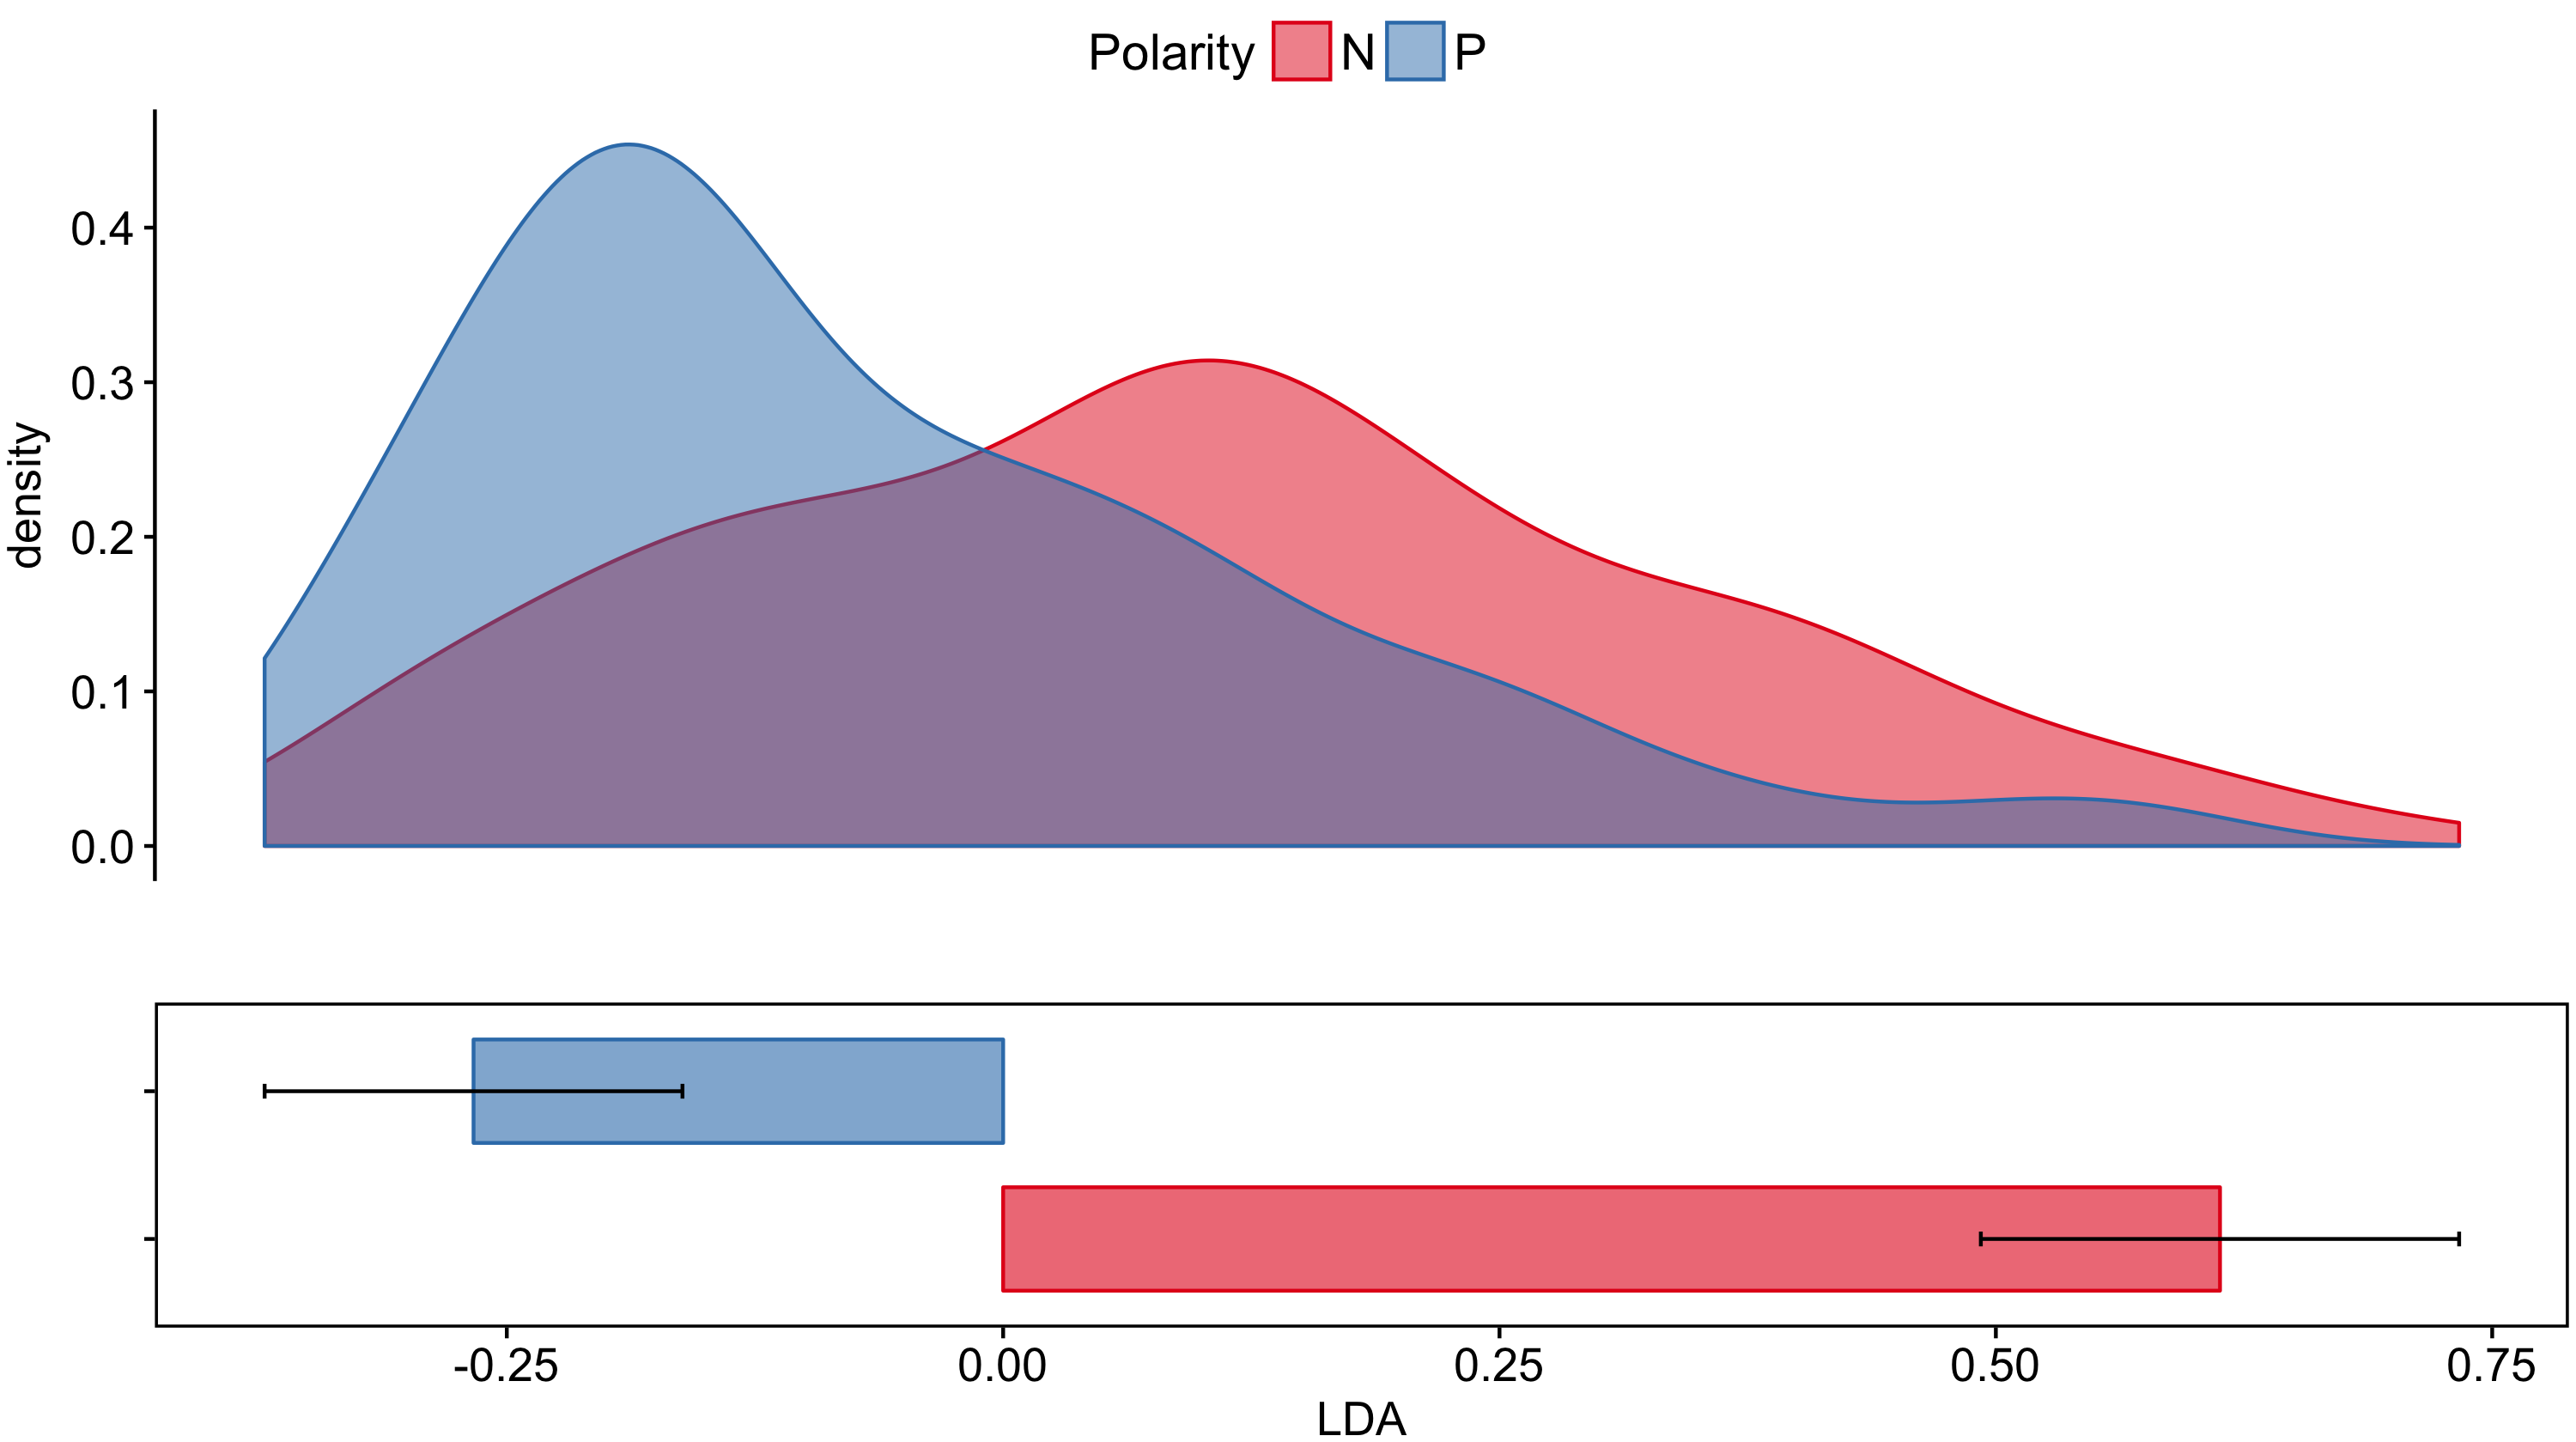
\includegraphics[width=\textwidth]{lda_distribution_negation.png}
\caption{LDA (coords, speed and acceleration) }
\end{subfigure}
\begin{subfigure}[b]{0.45\textwidth}
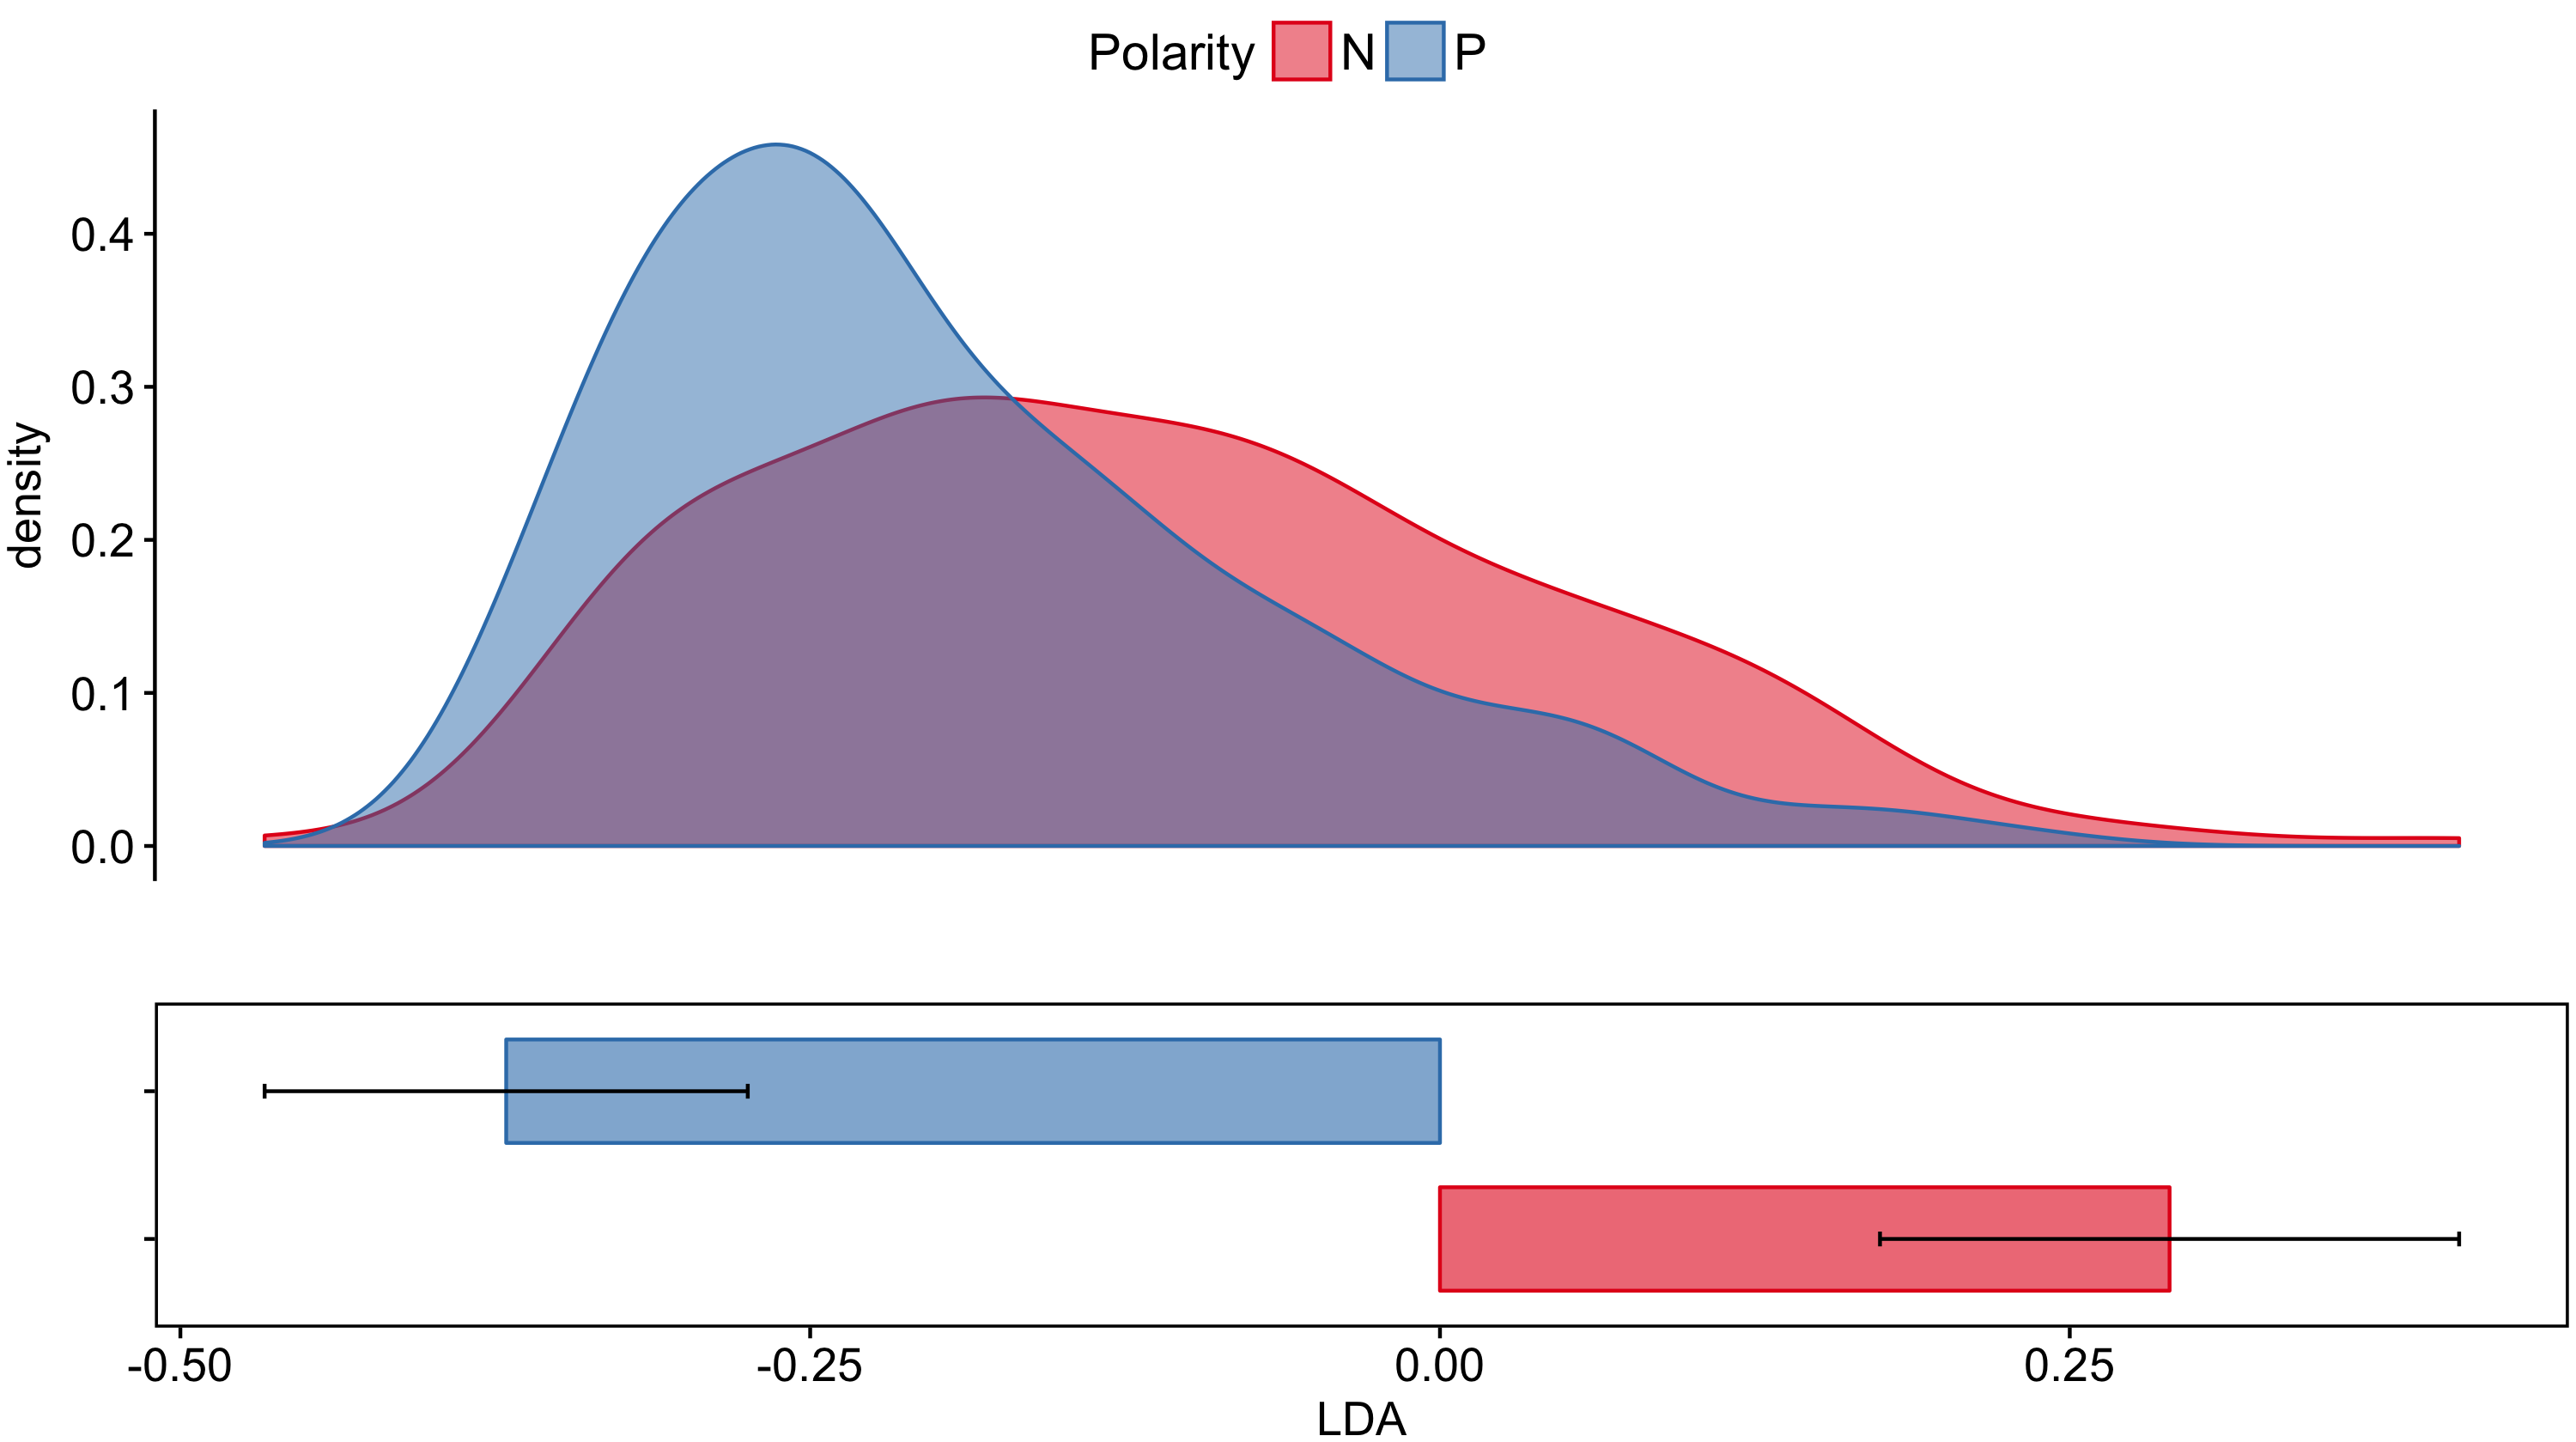
\includegraphics[width=\textwidth]{lda_coord_distribution_negation.png}
\caption{LDA only with coordinates}
\end{subfigure}
\caption{Two LDA classifiers applied to \textit{true} trials. }
\label{fig:lda_negation}
\end{figure}

To assess how well these classifiers separate positive from negative trials, we bootstrapped new samples from the original set of data (iterations=1000) and calculated the area under the ROC curve for the classification of each of these samples. 
In order to estimate the classification power, we evaluated the performance after reducing the sample size. \Cref{fig:permutation_AUC_negation}A shows the mean AUC values obtained after applying the same procedure to different sample sizes. 
Note that these values are generally lower that the ones obtained in the validation experiment. This is not surprising given that the classifier is being trained and tested with different sets of data, which target different cognitive processes. 

Could the observed performance be expected if negative and positive trials were actually not different from each other? Are these AUC values significantly different from the ones one would have obtained from applying the LDA to a set of data where there is no difference between experimental conditions (i.e. \emph{null hypothesis})? We calculated the AUC values for a set of data where experimental labels (positive, negative) were scrambled. The distribution of AUC values under the \emph{null hypothesis} was compared to the performance observed for the original set of data. \Cref{fig:permutation_AUC_negation}B illustrates the separability of the two classifications for each sample size.

\begin{figure}
\centering
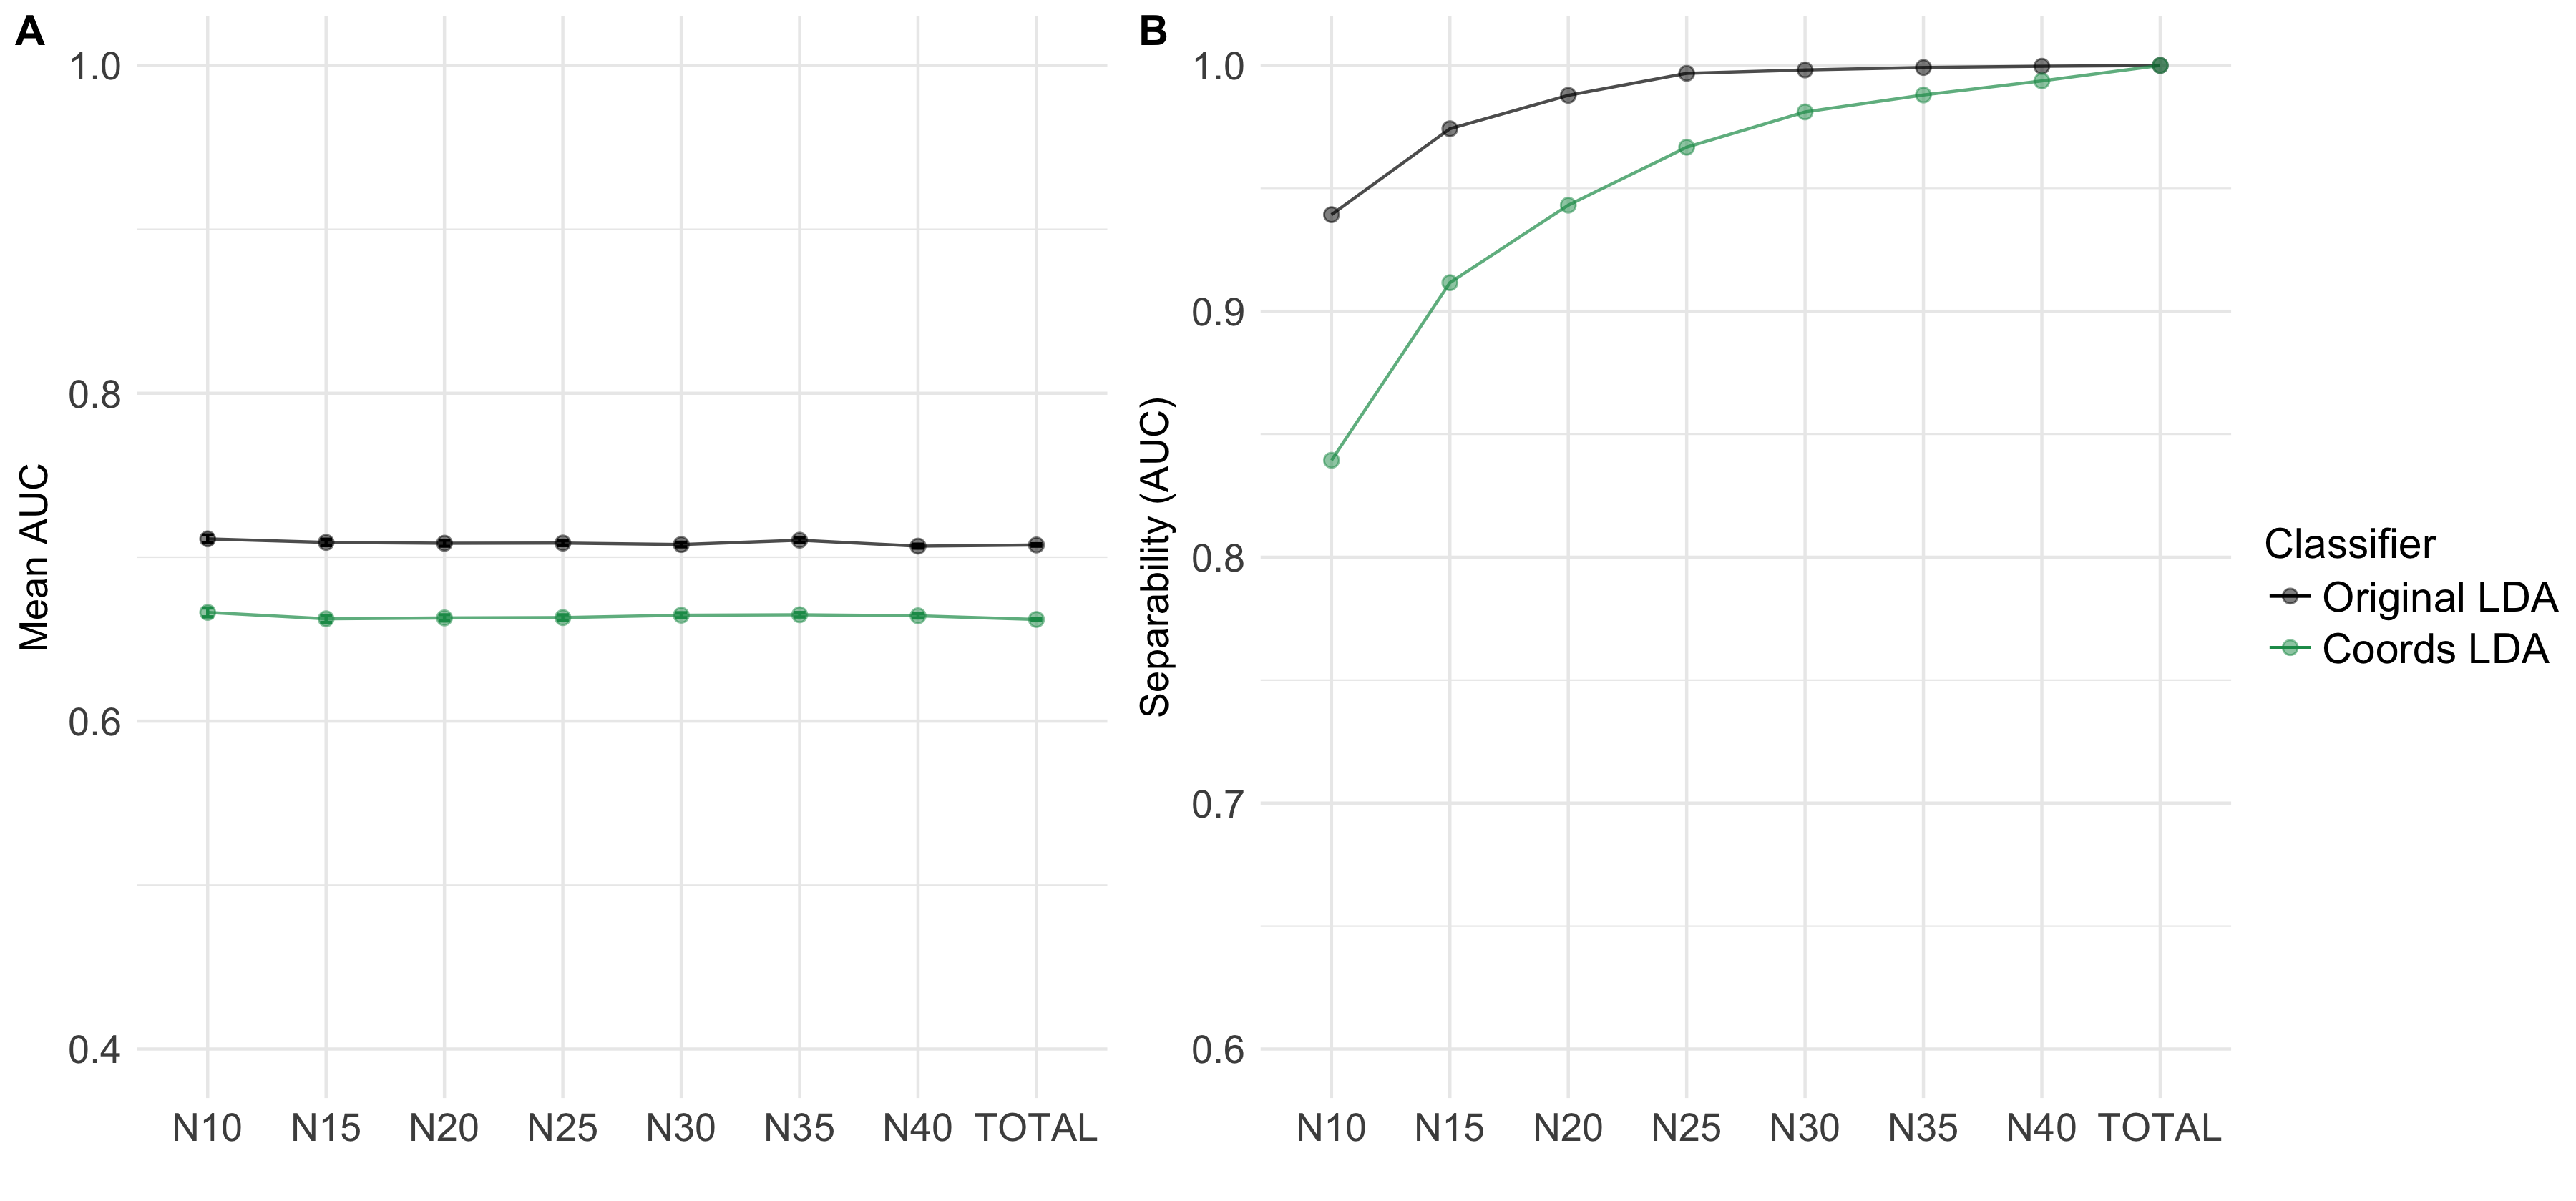
\includegraphics[width=\textwidth]{auc_permutation_negation_1.png}
\caption{\textbf{Performance of LDA classifiers.} A. Mean AUC values over bootstrapped data (iterations=1000) for different sample sizes;  B. Difference of classifier performance when applied to scrambled vs. original set of data.}
\label{fig:permutation_AUC_negation}
\end{figure}


The LDA classifier trained with ``quasi-decisions'' seems to make a relevant distinction between experimental conditions. This finding suggest that the contrast between negative and positive trials has something in common with the contrast between straightforward and switched trials from the validation experiment. The fact that negation has similar properties as pseudo “switched-decisions'' indicates that verifying negative sentences might underlie a change of decision, as proposed by Dale \& Duran (\citeyear{Dale2011}), among others.  
However, while mouse trajectories corresponding to negative and `switched' trials do share basic properties (e.g. shape), they seem to differ on how they are placed in the “change of decision” spectrum; namely, they occupy different parts of the quasi-decision-based LDA continuum (compare \Cref{DIST:LDA} and \Cref{fig:lda_negation}). This is not surprising given that we are dealing with different cognitive processes --very simple `quasi-decisions' vs. sentence-verification based decision. 

A last note should be made about the comparison between the two classifiers. While the classifiers' comparison in \Cref{DIST:AUC} indicated that relative spatio-temporal features, such as distance-based acceleration and speed, were not essential for the classification of `quasi-decisions', these features do seem to play a role in the classification of sentence-verification data. Indeed, \Cref{fig:permutation_AUC_negation} reveals that the \emph{full} classifier --which takes all features as predictors-- makes a better distinction than the simplified one.   

\paragraph{Other mouse-tracking measures}
In the validation experiment, the performance of the LDA classifier was shown to be significantly better than the one of other mouse-tracking measures. Does this difference remain when these measures are applied to the new experimental data (and hence to slightly different decision processes)? 
While it's true the LDA trained on validation data can make a distinction between negative and positive trials, it might not be the \emph{best} possible strategy for classification. 

We address the question of whether different measures differ on their ability to find the observed effect by applying the same procedure as before: we calculated the mean area under the ROC curve for different sample sizes (cf. \Cref{fig:permutation_AUC_negation_measures}A), and contrasted these values against the null hypothesis (i.e. the values we would have obtained if there had been no difference between the experimental conditions; \Cref{fig:permutation_AUC_negation_measures}B)\footnote{Interestingly, the ranking based on power does not correspond exactly to the one based on the AUC mean values: how good is each measure at detecting the effect is not necessarily equivalent to its absolute performance.}. 
%The distribution of each measure can be found in the Supplementary Materials. 

\begin{figure}
\centering
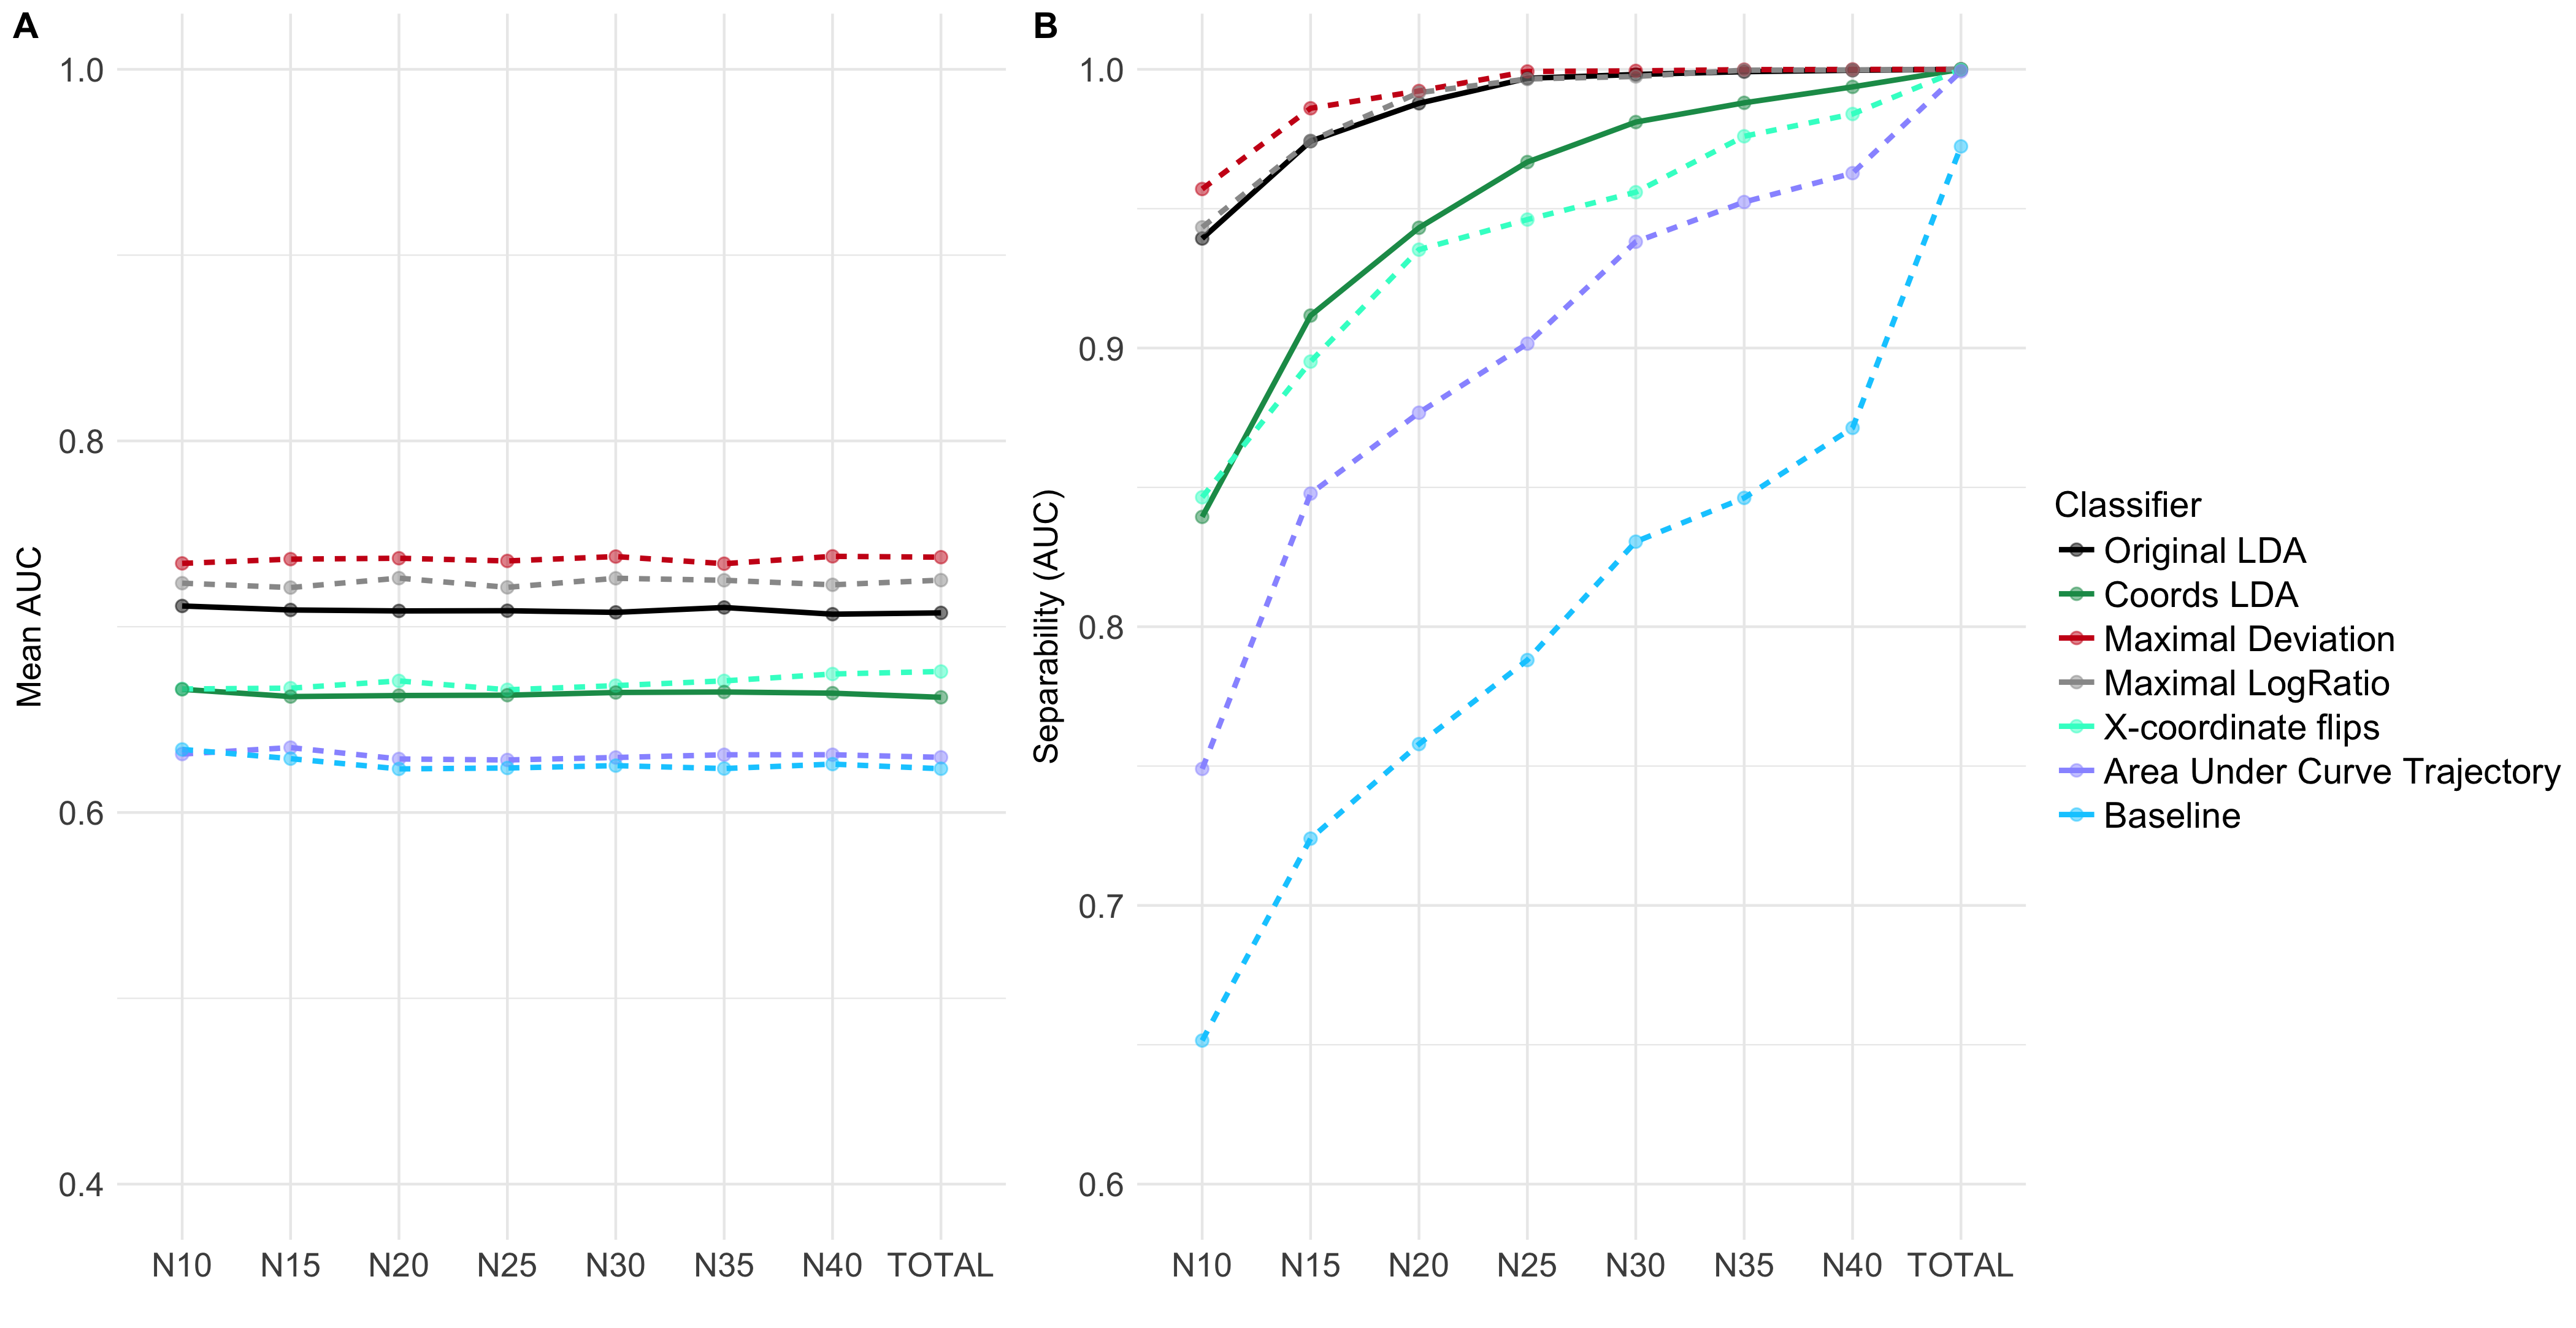
\includegraphics[width=\textwidth]{auc_permutation_negation_2.png}
\caption{Performance of other measures}
\label{fig:permutation_AUC_negation_measures}
\end{figure}

%The performance analysis 
The results in \Cref{fig:permutation_AUC_negation_measures}A suggest that most measures perform a worse classification than the one observed for the validation data (compare with \Cref{DIST:AUC2}). 
Given that a decrease in performance is attested across the board and not only for the classifiers trained with validation data, 
this difference must be driven by properties of the new data set. Specifically, the sentence-verification data might be more variable, such that both negative and positive trials might underlie instances of different decision processes. 

Moreover, the LDA classifier seems here to be as powerful as other traditional mouse-tracking measures, such as the Maximal Deviation and the Maximal LogRatio. This finding contrasts with the results of the validation experiment, opening the possibility of using any of these alternative measures to analyse mouse-tracking data from sentence verification tasks. Importantly, the classifier is still a better choice from a conceptual perspective, as long as it does not make any specific assumption about how the change of decision should be reflected by mouse-trajectories.  

\paragraph{Baseline}
Our LDA, trained to classify `quasi-decisions', can separate the two experimental conditions of Dale \& Duran's replication. We have interpreted this result by suggesting that the LDA is distinguishing mouse trajectories that underlie two different decision processes. 
Alternatively, one could argue that the classification made by the LDA is not based on decision processes, but on some other feature of mouse paths, which happens to be partially shared between conditions in both experiments. 
For example, the LDA might not be sensitive to decision shift but to cognitive cost, and the contrast between straightforward and switched trials, on one hand, and positive and negative trials, on the other, might have that in common. 


\begin{figure}
\centering
\begin{subfigure}[b]{0.45\textwidth}
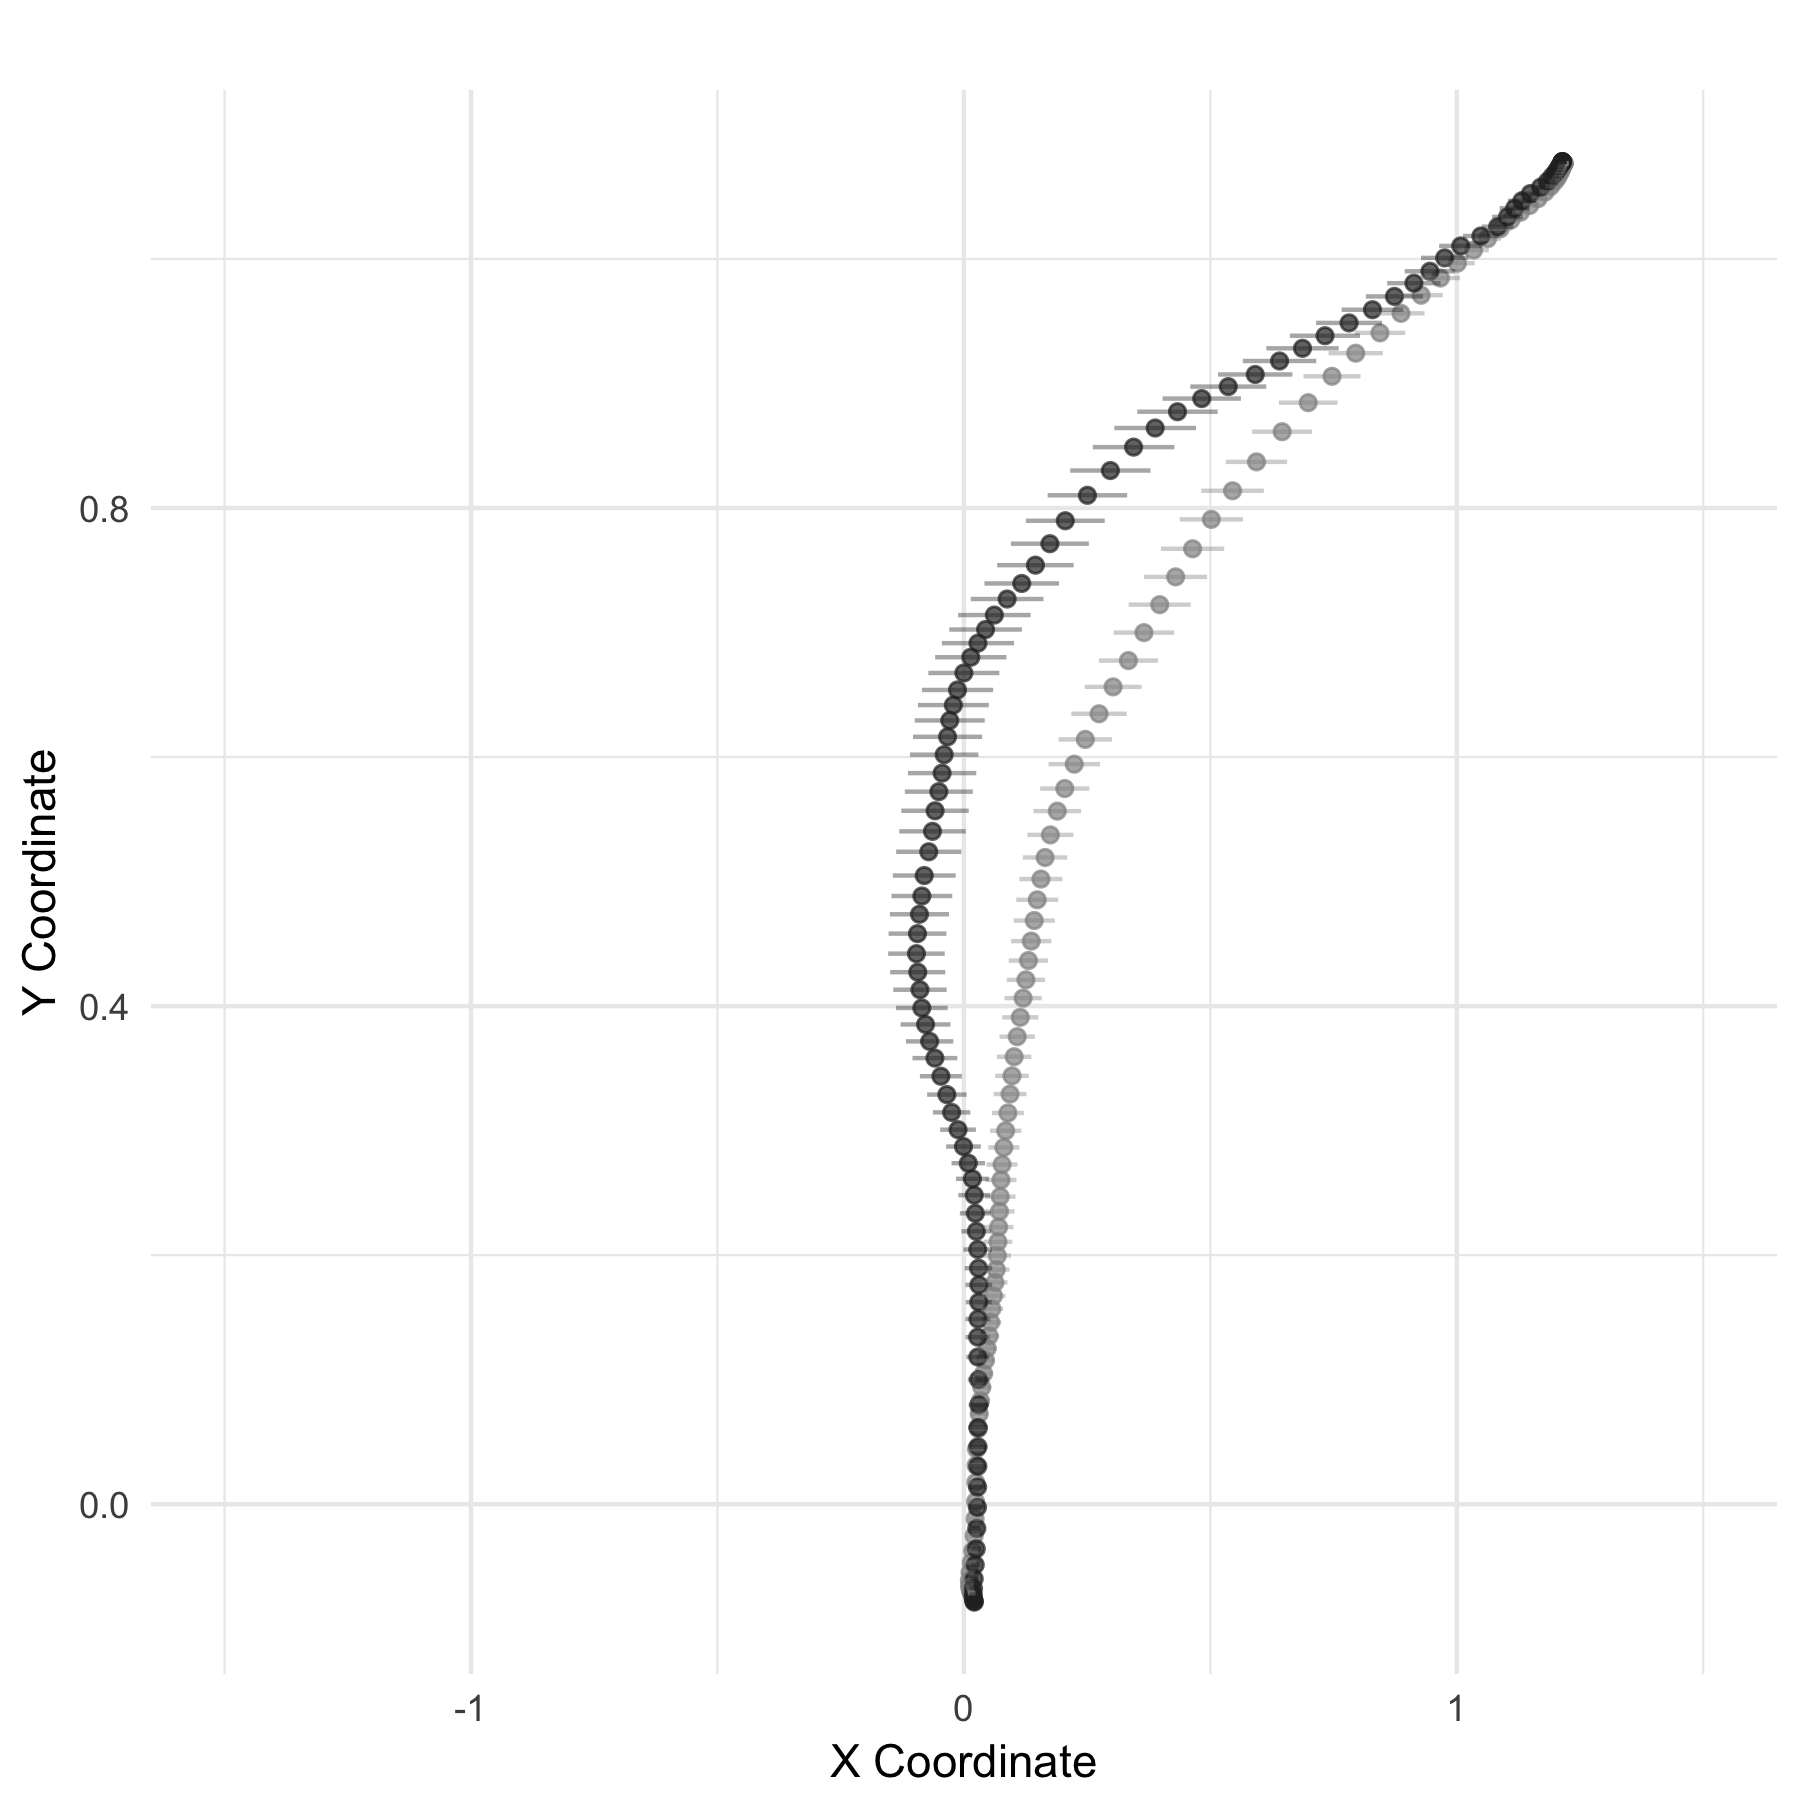
\includegraphics[width=\textwidth]{TrajectoriesBaseline.png}
\caption{Mean Trajectories}\label{fig:baseline-traj}
\end{subfigure}
\begin{subfigure}[b]{0.45\textwidth}
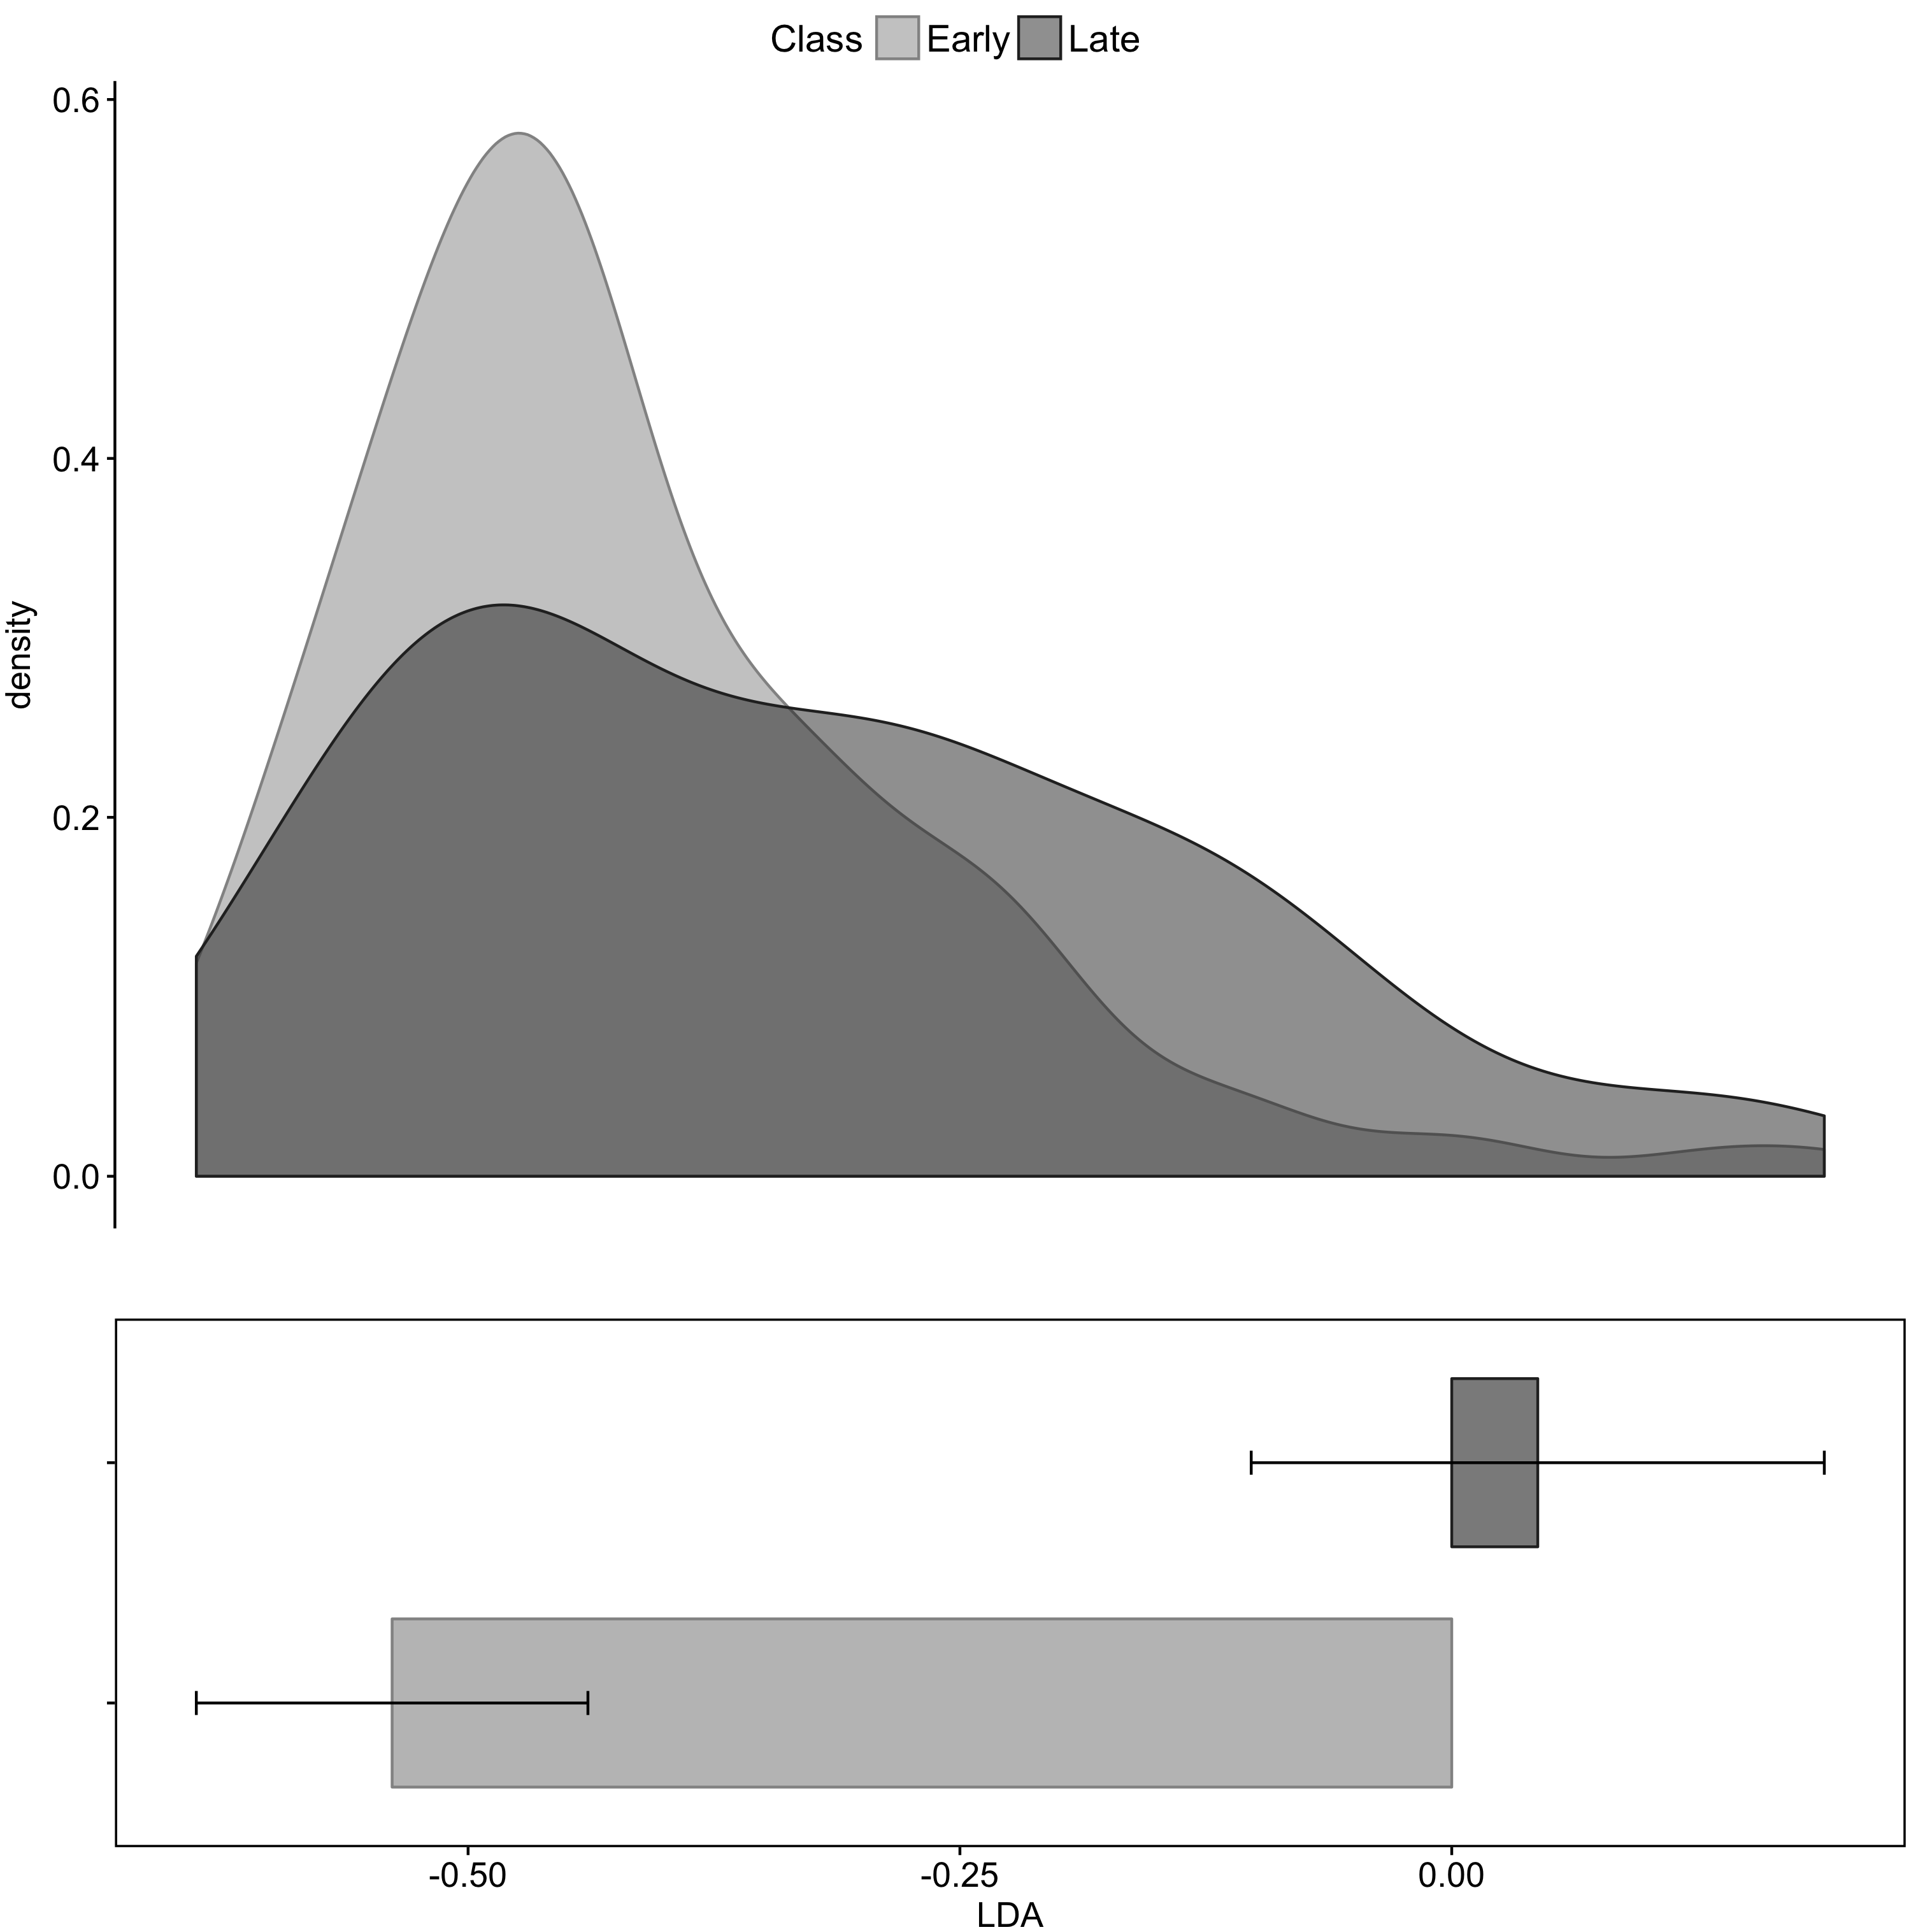
\includegraphics[width=\textwidth]{lda_distribution_baseline.png}
\caption{Mean and distribution of LDA measure}\label{fig:baseline-lda}
\end{subfigure}
\caption{Baseline data set}
\end{figure}

To disentangle these possibilities, we asked how our LDA classifies trajectories that might have different shapes but do not underlie two different decision processes (straightforward vs. switched), but a single one.
To this end, we constructed a \emph{baseline} set of data, which contained only positive trials from the original data set. These trials were further categorised into two classes depending on whether their response time was above or below the subject mean. We reasoned that shorter response times would correspond to an `early commitment' towards the answer, whereas longer response times would reflect a `late commitment'. Importantly, no trial in the \emph{baseline} data set was assumed to underlie a decision shift; thus, the LDA was expected to perform a poor classification.  

As illustrated by mean trajectories in \Cref{fig:baseline-traj}, the two classes in the baseline data have slightly different trajectory shapes.
The distribution of the LDA measure after testing the classifier on the new data set is shown in \Cref{fig:baseline-lda}. The performance was evaluated following the same procedure applied above (see blue line in \Cref{fig:permutation_AUC_negation_measures}). 

The classification on `early' and `late' categories is less accurate than the one performed in the original data set, to separate negative and positive trials.
Differences in trajectories that are not due to the experimental manipulation are poorly captured by the LDA measure: even trajectories that do have some properties in common with \emph{switched} and \emph{negation} trials are not taken to be underlying a change of decision. 
These findings suggest that our classifier is not just tapping onto trajectory similarity but onto decision processes reflected on mouse trajectories.

\section{Conclusion/General discussion}

We aimed to investigate the connection between action and cognition by testing one of its specific instances: the mapping of decision making processes into mouse movements. Our findings make three main contributions on this point. 

First, by manipulating whether the stimulus triggered or not a change of decision, we have shown --for the first time in a direct way-- that mouse trajectories reflect basic decision processing: When participants were forced to change their answer, this switch had a systematic/direct mapping/impact on hand movements (\Cref{section:validation}). 

Second, we trained a LDA classifier with mouse-trajectories underlying these `quasi-decisions' to determinate whether or not a given trial involved a decision shift. 
This LDA has been proven to accurately classify not only paths corresponding to other quasi-decisions', but also mouse-trajectories underlying more complex decision processes, such as sentence verification. While the performance of the classifier --at this stage-- might be as good as the one of other commonly used mouse-tracking measures (i.e. Maximal Deviation), it has the unique advantage of not relying on any specific assumption about how trajectories should look like. Indeed, we demonstrated that the LDA classifier is not just sensitive to superficial similarity between trajectories, but to the underlying cognitive processes. 

Lastly, our results also contribute to the research in negation processing. Besides replicating Dale \& Duran' experiment, the classification performed by the LDA suggests that verifying negative sentences involves a decision shift, similar to the one used for the training. We then provide new evidence to the hypothesis that processing negated sentences --at least in out-of-the-blue contexts-- involves a two-step derivation, where the positive argument is initially computed.  

%

To conclude, we should mention that the differences in the LDA performance across the two experiments can be well understood by noticing that two data sets capture slightly different decision processes. In order to capture more subtle contrasts in decision making, the training data should contain more variation. Further research will explore this possibility. 
    


\section{Supplementary Materials}

\bibliography{biblio}


\end{document}
